%% abtex2-modelo-trabalho-academico.tex, v-1.9.2 laurocesar
%% Copyright 2012-2014 by abnTeX2 group at http://abntex2.googlecode.com/ 
%%
%% This work may be distributed and/or modified under the
%% conditions of the LaTeX Project Public License, either version 1.3
%% of this license or (at your option) any later version.
%% The latest version of this license is in
%%   http://www.latex-project.org/lppl.txt
%% and version 1.3 or later is part of all distributions of LaTeX
%% version 2005/12/01 or later.
%%
%% This work has the LPPL maintenance status `maintained".
%% 
%% The Current Maintainer of this work is the abnTeX2 team, led
%% by Lauro César Araujo. Further information are available on 
%% http://abntex2.googlecode.com/
%%
%%
% ------------------------------------------------------------------------
% ------------------------------------------------------------------------
% abnTeX2: Modelo de Trabalho Academico (tese de doutorado, dissertacao de
% mestrado e trabalhos monograficos em geral) em conformidade com 
% ABNT NBR 14724:2011: Informacao e documentacao - Trabalhos academicos -
% Apresentacao - Adaptado para o padrão do Departamento de Políticas Públicas da UFRN
%por Moacir Hardt Godoy - 2015
% ------------------------------------------------------------------------
% ------------------------------------------------------------------------

\documentclass[
	% -- opções da classe memoir --
	12pt,				% tamanho da fonte
	openright,			% capítulos começam em pág ímpar (insere página vazia caso preciso)
	twoside,			% para impressão em frente e verso. Oposto a oneside
	a4paper,			% tamanho do papel. 
	% -- opções da classe abntex2 --
	chapter=TITLE,		% títulos de capítulos convertidos em letras maiúsculas
	section=TITLE,		% títulos de seções convertidos em letras maiúsculas
	subsection=TITLE,	% títulos de subseções convertidos em letras maiúsculas
	subsubsection=TITLE,% títulos de subsubseções convertidos em letras maiúsculas
	% -- opções do pacote babel --
	spanish,            % idioma adicional para hifenização
	english,			% idioma adicional para hifenização
	brazil				% o último idioma é o principal do documento
	]{abntex2}

% ---
% Pacotes básicos 
% ---
\usepackage[adobe-utopia]{mathdesign}			% Usa a fonte Utopia + o pacote de simbolos matemáticos			
\usepackage[T1]{fontenc}		% Selecao de codigos de fonte.
\usepackage[utf8]{inputenc}	    % Codificacao do documento (conversão automática dos acentos)
\usepackage{lastpage}			% Usado pela Ficha catalográfica
\usepackage{indentfirst}
\usepackage{parskip}	    	% Indenta o primeiro parágrafo de cada seção.
\usepackage[usenames]{color}	% Controle das cores
\usepackage{graphicx}			% Inclusão de gráficos
\usepackage{microtype} 			% para melhorias de justificação
\usepackage{pdfpages}           % para inserir arquivos pdf
\usepackage{placeins}
\usepackage{tikz}               % para inserir figuras complicadas
\usepackage{lettrine}           % a primeira letra de cada seção ocupa 2 linhas
\usepackage{calligra}		    % Letras manuscritas
\usepackage[pages=some]{background}%Coloca um texto em background


% Pacotes de citações
% ---
\usepackage[brazilian,hyperpageref]{backref}	 % Paginas com as citações na bibl
\usepackage[alf]{abntex2cite}
%\usepackage[alf,abnt-etal-cite=4]{abntex2cite}	% Citações padrão ABNT sistema alfabético e et al para mais de 3 autores NBR 6023 8.1.1.1
\usepackage{hyperref}
% --- 
% CONFIGURAÇÕES DE PACOTES
% --- 
% ---
% Configurações do pacote backref
% Usado sem a opção hyperpageref de backref
\renewcommand{\backrefpagesname}{Citado na(s) página(s):~}
% Texto padrão antes do número das páginas
\renewcommand{\backref}{}
% Define os textos da citação
\renewcommand*{\backrefalt}[4]{
	\ifcase #1 %
		Nenhuma citação no texto.%
	\or
		Citado na página #2.%
	\else
		Citado #1 vezes nas páginas #2.%
	\fi}%
% ---

% ---
% Informações de dados para CAPA e FOLHA DE ROSTO
% --
\titulo{Entre o desvio, o crime e a tolerância zero: estudo da percepção ao cumprimento das leis no município de Natal-RN}
\autor{Moacir Hardt Godoy}
\local{Natal-RN}
\data{2015}
\orientador[Orientadora:]{Profa. Dra. Zoraide Souza Pessoa}

%\Refaz a capa  e a folha de rosto para colocar no padrão do DPP/ UFRN (que não é exatamente o da ABNT)
\renewcommand{\imprimircapa}{%
	\begin{capa}%
	\begin{tikzpicture}[remember picture,overlay]
	\node[yshift=-35mm,xshift=35mm] at
	(current page.north west)
	{
\includegraphics[width=25mm]{ufrn}}; 
	\end{tikzpicture}
	
	\vspace*{-20mm}
	
	%\vspace{20mm}
	\centering
	{\indent\bfseries UNIVERSIDADE FEDERAL DO RIO GRANDE DO NORTE}
	
	{\indent\bfseries CENTRO DE CIÊNCIAS HUMANAS, LETRAS E ARTES}
	
	{\indent\bfseries DEPARTAMENTO DE POLÍTICAS PÚBLICAS}
	
	{\indent\bfseries CURSO DE GESTÃO DE POLÍTICAS PÚBLICAS}
	
		\centering
		\vspace*{1cm}
\textbf{{\ABNTEXchapterfont\Large\imprimirautor}}
		
		\vfill
		\ABNTEXchapterfont\bfseries\LARGE\imprimirtitulo
		\vfill
		
		\large\imprimirlocal
		
		\large\imprimirdata
		
		\vspace*{1cm}
		\end{capa}
	}
\renewcommand{\imprimirfolhaderosto}{
	\begin{center}
		
		%\vspace*{1cm}
		{\ABNTEXchapterfont\large\imprimirautor}
		
		\vspace*{\fill}\vspace*{\fill}
		\begin{center}
			\ABNTEXchapterfont\bfseries\Large\imprimirtitulo
		\end{center}
		\vspace*{\fill}
		\hspace{.45\textwidth}
		\begin{minipage}{.5\textwidth}
				%\SingleSpacing
				\imprimirpreambulo
				\\\\ Orientadora: 
				\imprimirorientador
		\end{minipage}%
			\vspace*{\fill}
	
		
		{\large\imprimirlocal}
		\par
		{\large\imprimirdata}
		\vspace*{1cm}
		
	\end{center}
}
% Esse é um modo de comentar um grande trecho de código
\begin{comment}
\instituicao{%
  Universidade Federal do Rio Grande do Norte
  \par
  Centro de Ciências Humanas, Letras e Artes
  \par
  Departamento de Políticas Públicas
  \par
  Curso de Gestão de Políticas Públicas}
  \end{comment}
  
\tipotrabalho{Monografia final}
% O preambulo deve conter o tipo do trabalho, o objetivo, 
% o nome da instituição e a área de concentração 
\preambulo{Trabalho de Conclusão de Curso apresentado ao
	Curso Superior de Bacharelado em Gestão de
	Políticas Públicas da Universidade Federal do Rio
	Grande do Norte, em cumprimento às exigências
	legais como requisito parcial à obtenção do título
	de Bacharel em Gestão de Políticas Públicas.
	}
% ---
% ---
% Configurações de aparência do PDF final

% alterando o aspecto da cor azul
\definecolor{blue}{RGB}{41,5,195}

% informações do PDF
\makeatletter
\hypersetup{
     	%pagebackref=true,
		pdftitle={\@title}, 
		pdfauthor={\@author},
    	pdfsubject={\imprimirpreambulo},
	    pdfcreator={LaTeX with abnTeX2},
		pdfkeywords={Índice de Percepção das Leis}{Cidades}{Natal - RN}{Gestão de Políticas Públicas}, 
		colorlinks=true,       		% false: boxed links; true: colored links
    	linkcolor=blue,          	% color of internal links
    	citecolor=blue,        		% color of links to bibliography
    	filecolor=magenta,      		% color of file links
		urlcolor=blue,
		bookmarksdepth=4
}
\makeatother
% --- 
% Novo list of para Gráficos

\newcommand{\graficoname}{Gráfico}
\newcommand{\listofgraficosname}{Lista de gráficos}

\newfloat[chapter]{grafico}{loq}{\graficoname}
\newlistof{listofgraficos}{loq}{\listofgraficosname}
\newlistentry{grafico}{loq}{0}

% configurações para atender às regras da ABNT
\counterwithout{grafico}{chapter}
\renewcommand{\cftgraficoname}{\graficoname\space} 
\renewcommand*{\cftgraficoaftersnum}{\hfill--\hfill}

% Novo list of para Mapas

\newcommand{\mapaname}{Mapa}
\newcommand{\listofmapasname}{Lista de mapas}

\newfloat[chapter]{mapa}{lom}{\mapaname}
\newlistof{listofmapas}{lom}{\listofmapasname}
\newlistentry{mapa}{lom}{0}

% configurações para atender às regras da ABNT
\counterwithout{mapa}{chapter}
\renewcommand{\cftmapaname}{\mapaname\space} 
\renewcommand*{\cftmapaaftersnum}{\hfill--\hfill}

% Novo list of para Fotografias

\newcommand{\fotoname}{Foto}
\newcommand{\listoffotosname}{Lista de fotos}

\newfloat[chapter]{foto}{lop}{\fotoname}
\newlistof{listoffotos}{lop}{\listoffotosname}
\newlistentry{foto}{lop}{0}

% configurações para atender às regras da ABNT
\counterwithout{foto}{chapter}
\renewcommand{\cftfotoname}{\fotoname\space} 
\renewcommand*{\cftfotoaftersnum}{\hfill--\hfill}

% --- 
% Espaçamentos entre linhas e parágrafos 
% --- 

% O tamanho do parágrafo é dado por:
\setlength{\parindent}{1.3cm}

% Controle do espaçamento entre um parágrafo e outro:
\setlength{\parskip}{0.2cm}  % tente também \onelineskip

% ---
% compila o indice
% ---
\makeindex
% ---
% ----
% Início do documento
% ----
%
\begin{document}
% Seleciona o idioma do documento (conforme pacotes do babel)
%\selectlanguage{english}
\selectlanguage{brazil}

% Retira espaço extra obsoleto entre as frases.
\frenchspacing 
\setlength{\parskip}{0.5\baselineskip plus2pt minus2pt}
% ----------------------------------------------------------
% ELEMENTOS PRÉ-TEXTUAIS
% ----------------------------------------------------------
\pretextual

% ---
% Capa
% ---
\imprimircapa
% ---

% ---
% Folha de rosto
% (o * indica que haverá a ficha bibliográfica)
% ---
\imprimirfolhaderosto*


% Inserir a ficha catalografica
% ---

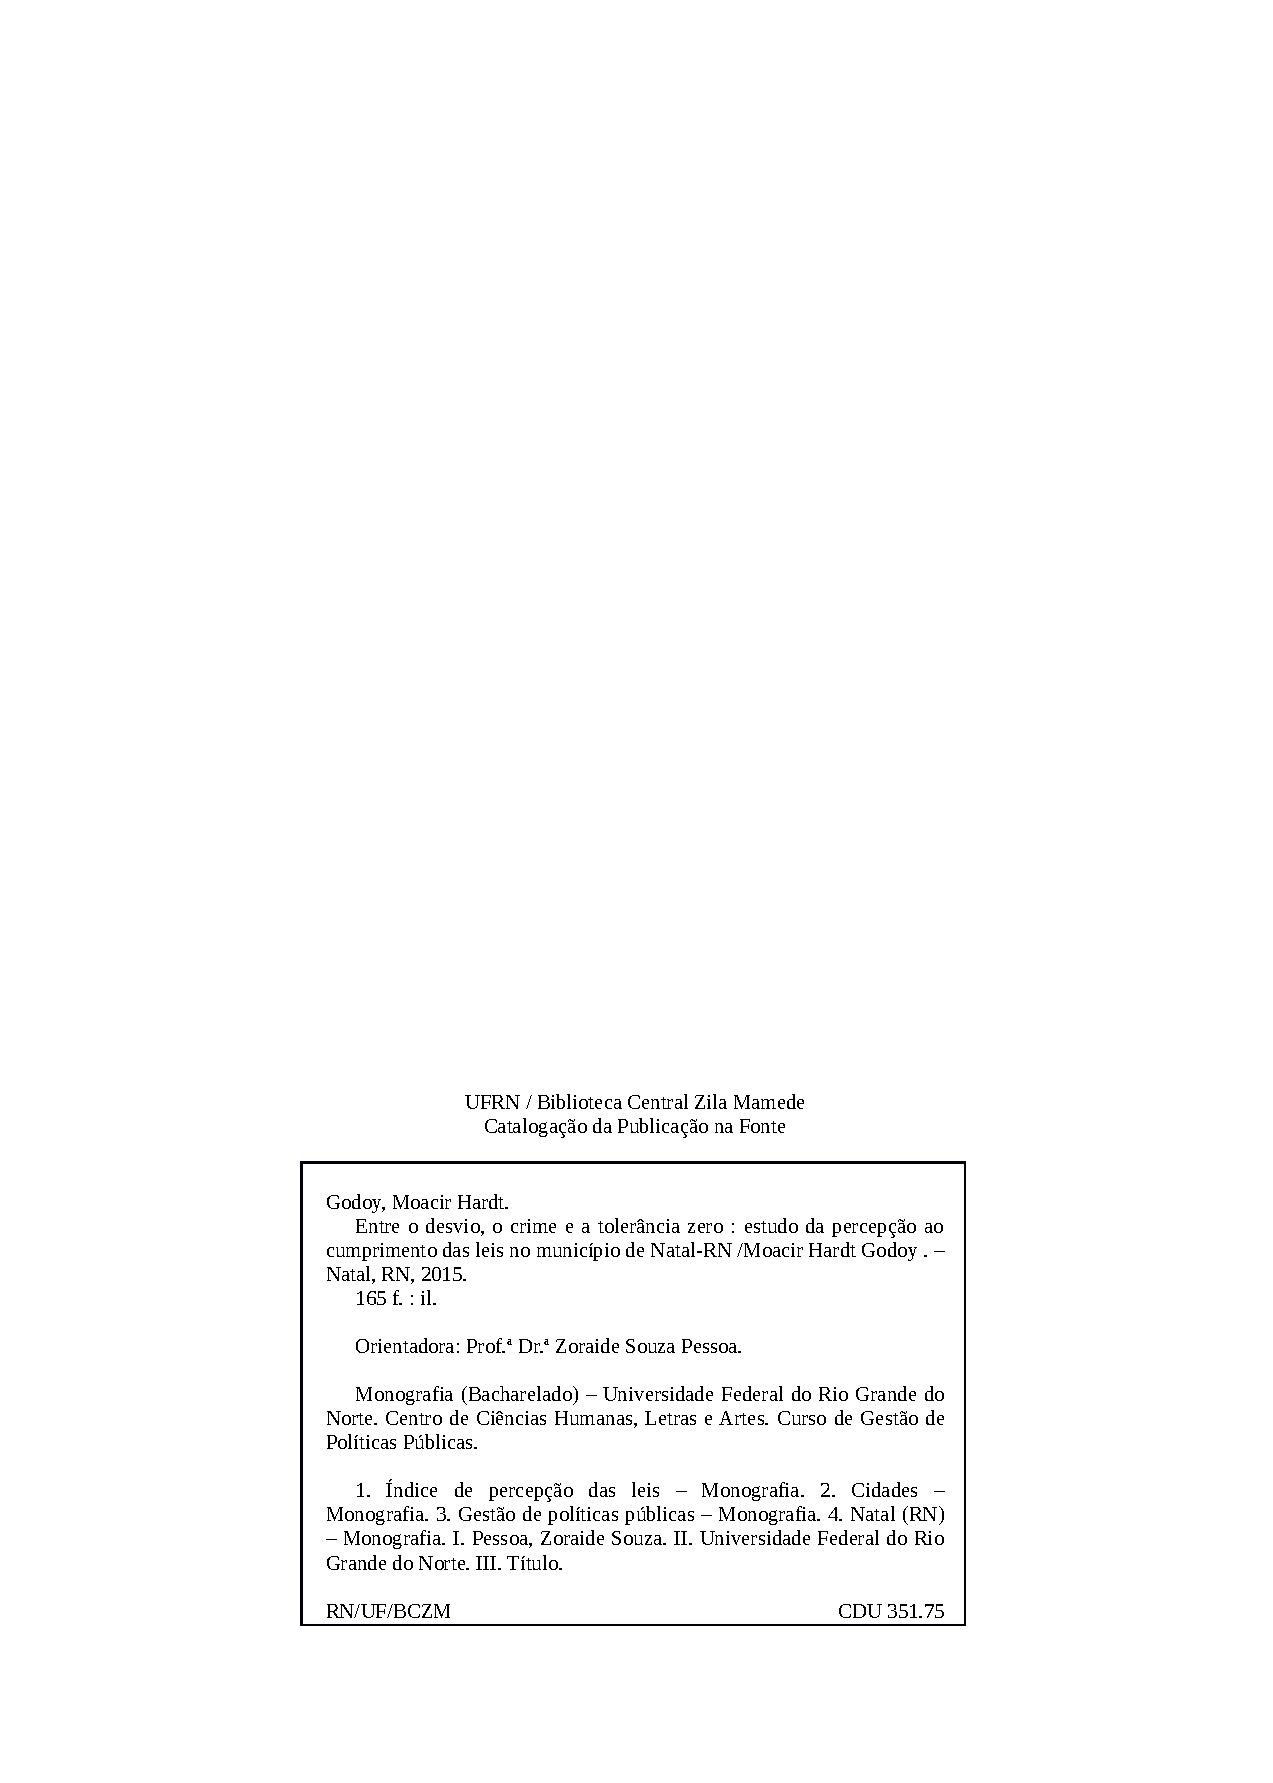
\includepdf{ficha_catalografica.pdf}%Fornecida pela biblioteca da UFRN

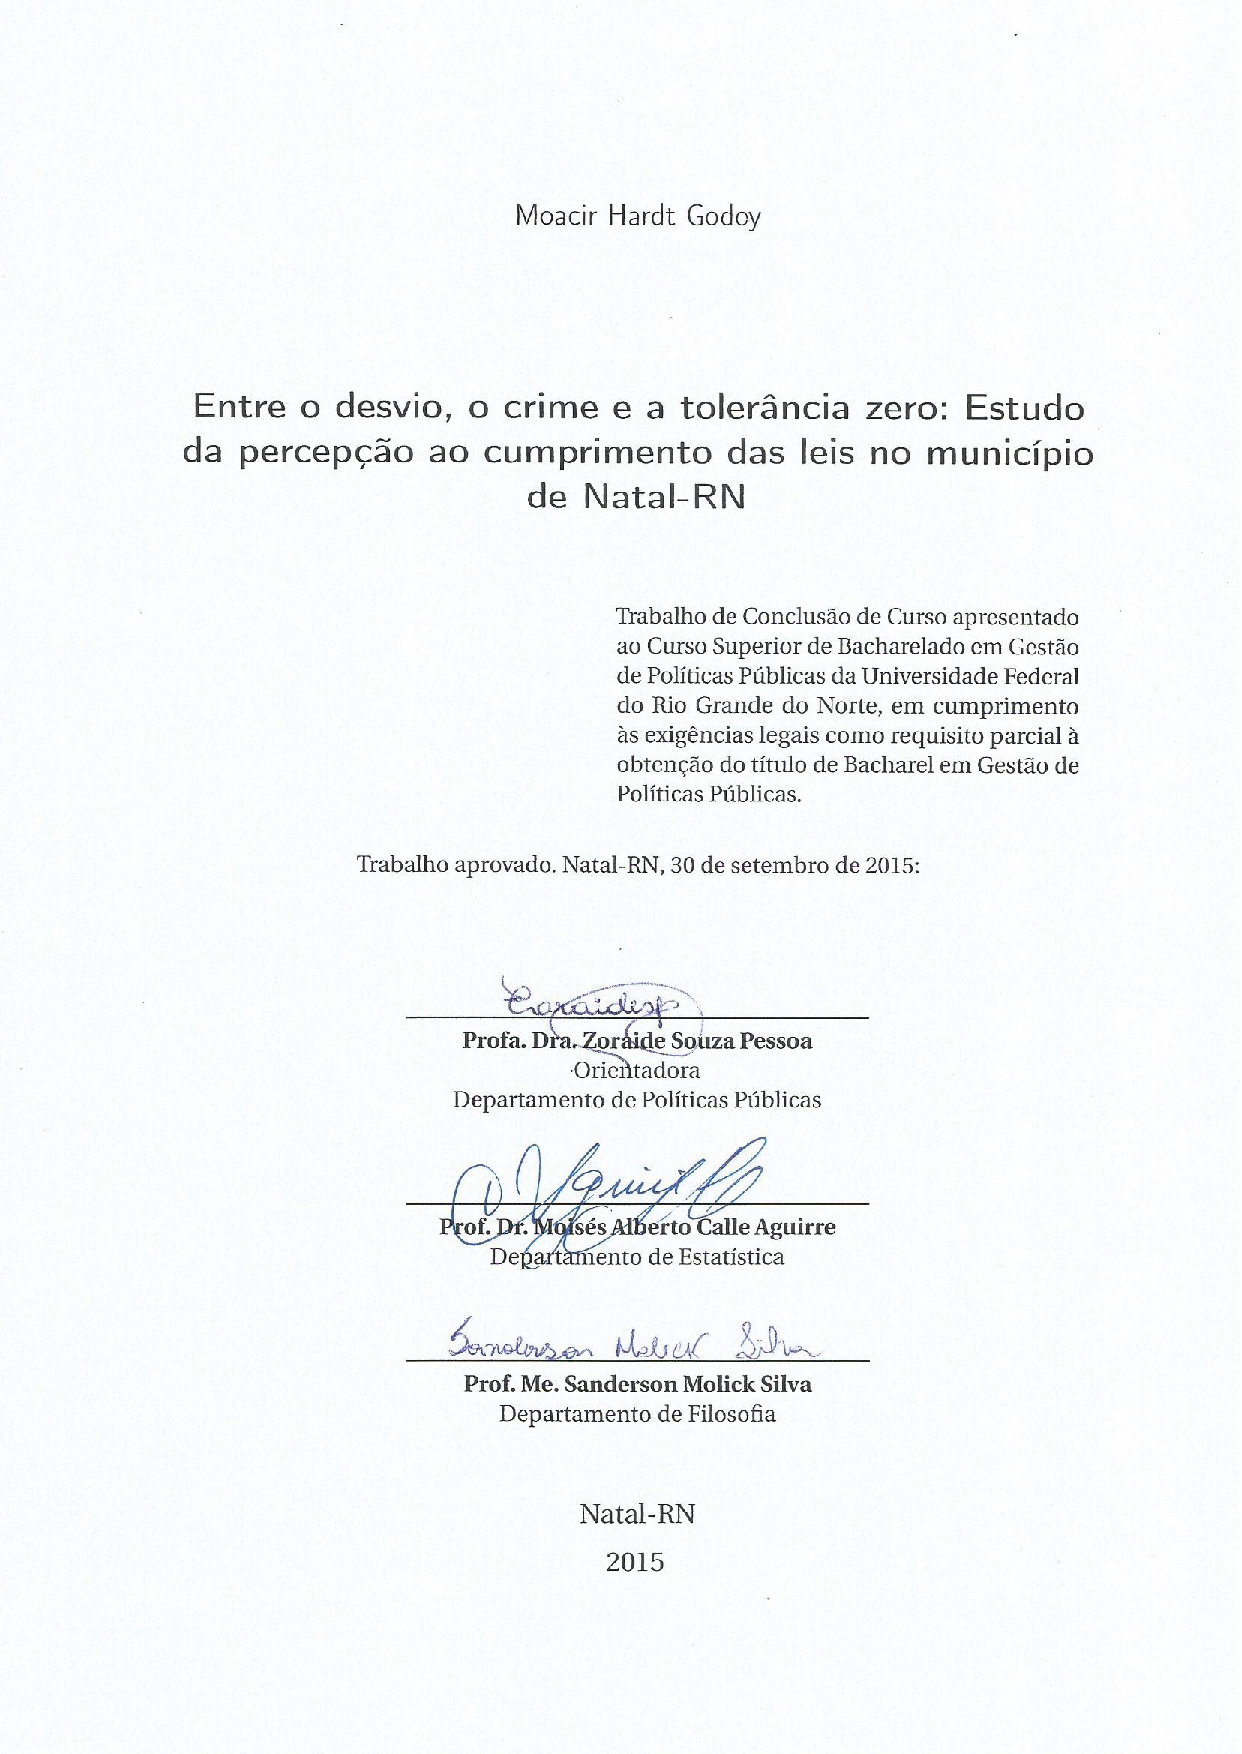
\includepdf{aprovacao1.pdf}

\cleardoublepage

% Os comandos \iffalse e \fi são outra forma de delimitar grandes espaços que não serão compilados
% Isto é um exemplo de Ficha Catalográfica, ou ``Dados internacionais de
% catalogação-na-publicação"". Você pode utilizar este modelo como referência. 
% Porém, provavelmente a biblioteca da sua universidade lhe fornecerá um PDF
% com a ficha catalográfica definitiva após a defesa do trabalho. 
\iffalse
\newpage
\backgroundsetup{placement=bottom,	hshift=10,
	vshift=10,angle=45,contents=Exemplo,color=yellow}
\BgThispage
\begin{fichacatalografica}
	\sffamily
	\vspace*{\fill}					% Posição vertical
	\begin{center}					% Minipage Centralizado
		\fbox{\begin{minipage}[c][8cm]{13.5cm}		% Largura
				\small
				\imprimirautor
				%Sobrenome, Nome do autor
				
				\hspace{0.5cm} \imprimirtitulo  / \imprimirautor. --
				\imprimirlocal, \imprimirdata-
				
				\hspace{0.5cm} \pageref{LastPage} p. : il. (algumas color.) ; 30 cm.\\
				
				\hspace{0.5cm} \imprimirorientadorRotulo~\imprimirorientador\\
				
				\hspace{0.5cm}
				\parbox[t]{\textwidth}{\imprimirtipotrabalho~--~\imprimirinstituicao,
					\imprimirdata.}\\
				
				\hspace{0.5cm}
				1. Índice de Percepção das Leis.
				2. Cidades.
				3. Natal (RN).
				4. Gestão de Políticas Públicas.
				I. Profa. Dra. Zoraide Souza Pessoa.
				II. Universidade Federal do Rio Grande do Norte.
				III. Departamento de Políticas Públicas.
				IV. Curso de Gestão de Políticas Públicas.
				V. Entre o desvio, o crime e a tolerância zero: Estudo da percepção ao cumprimento das leis no município de Natal-RN\\ 			
				
				\hspace{8.75cm} CDU XX:XXX:xxx.x\\
			\end{minipage}}
		\end{center}
\end{fichacatalografica}

% ---
% ---
% Inserir folha de aprovação
% ---

% Isto é um exemplo de Folha de aprovação, elemento obrigatório da NBR
% 14724/2011 (seção 4.2.1.3). Você pode utilizar este modelo até a aprovação
% do trabalho. Após isso, substitua todo o conteúdo deste arquivo por uma
% imagem da página assinada pela banca com o comando abaixo:
%

%
\begin{folhadeaprovacao}

  \begin{center}
    {\ABNTEXchapterfont\large\imprimirautor}

    \vspace*{\fill}\vspace*{\fill}
    \begin{center}
      \ABNTEXchapterfont\bfseries\Large\imprimirtitulo
    \end{center}
    \vspace*{\fill}
    
    \hspace{.45\textwidth}
  \begin{minipage}{.5\textwidth}
        \imprimirpreambulo
   \end{minipage}%
    \vspace*{\fill}
    Trabalho aprovado. \imprimirlocal, 30 de setembro de 2015:
    \end{center}
   
   \assinatura{\textbf{\imprimirorientador} \\ Orientadora \\  Departamento de Políticas Públicas} 
   \assinatura{\textbf{Prof. Dr. Moisés Alberto Calle Aguirre} \\ Departamento de Estatística}
   \assinatura{\textbf{Prof. Me. Sanderson Molick Silva} \\ Departamento de Filosofia}  
   \begin{center}
    \vspace*{0.5cm}
    {\large\imprimirlocal}
    \par
    {\large\imprimirdata}
    \vspace*{1cm}
  \end{center}
\end{folhadeaprovacao}
% ---
\fi
% ---
% Dedicatória
% ---
\begin{dedicatoria}
\centering

\textbf{Zona Norte, Zona Sul\\
Khrystal Saraiva}\\
       
     {\calligra Eu quero ir\\
       Da Zona Norte a Zona Sul\\
       Quero atravessar a ponte e me sentir num só lugar\\
       
       Quero tomar banho de rio\\
       Quero tomar banho de mar\\
       Quero saúde e respeito\\
       Pro povo em todo lugar\\
       
       Pajuçara, Igapó\\
       Potengi, o meu Gramoré\\
       Do lado que eu quero morar\\
       Se vive na base da fé\\
       
       Santa Catarina abençoa\\
       Panatis e Santarém\\
       E a Itapetinga nos leva\\
       As fronteiras da Nova Natal\\
       
       Não tape o sol com a peneira\\
       Maquiando o cartão postal\\
       Me olhe dentro dos olhos\\
       Me trate de igual pra igual\\
       
       De que lado mora o seu preconceito\\
       Atravesse a ponte que eu vou lhe mostrar\\
       
       E de que lado mora\\
       O seu preconceito\\
       Atravesse a ponte que eu vou...\\
       
       Salve a galera da avenida Pompéia\\
       Por onde eu passo, bem dizer toda semana\\
       Pra pedir a benção da minha mãe, Dona Maria\\
       
       E agora quero estender meu alô pra rapaziada do Pajuçara,\\
       Cidade Praia, Parque dos Coqueiros, Galera de Santa Rita,\\
       Alvorada, Vale Dourado, Parque das Dunas, Brasil Novo,\\
       Vila Verde, alô alô Gramorezinho! São Gonçalo do Amarante, Planalto,\\ toda rapaziada do Sarney, Golandim, Sopapo, Alto da torre, África...\\
       
       De que lado mora o seu preconceito?\\
       De que lado mora?\\
       O seu preconceito?\\
       De que lado mora?\\
       De que lado mora o seu preconceito?}
\end{dedicatoria}
% ---

% ---
% Agradecimentos NBR 14724:2011 subitem 4.2.1.4
% ---
\begin{agradecimentos}
\lettrine[lines=2, lhang=0.33, loversize=0.25]{I}{nicialmente}, agradeço ao “ser do qual nada maior pode ser pensado”, por me dar uma segunda chance de vida e mostrar que eu ainda tenho missões a cumprir nesse mundo. Que este trabalho represente a finalização de mais uma delas.
\par
A minha esposa Simone Hardt Godoy pela compreensão e tolerância das muitas e longas horas “ausente” à frente do computador.
\par
A minha orientadora, Profa. Dra. Zoraide Souza Pessoa pela paciência e dedicação em muitos meses de orientação, sempre indicando os melhores caminhos para consolidar o presente trabalho.
\par
Aos meus mestres do curso de Gestão de Políticas Públicas da UFRN que moldaram minha mente na mudança da percepção de um mundo voltado às ciências exatas para um mundo real e humanitário. 
\par
Finalmente, aos milhares de anônimos que se empenham na criação, implantação e distribuição de software
de domínio público  O presente trabalho foi feito usando o sistema operacional Debian
\url{https://www.debian.org/index.pt.html}, com o processador de textos \LaTeX\
\url{http://www.latex-project.org/} e o tratamento estatístico usando PSPP
\url{http://www.gnu.org/software/pspp/} - uma versão livre do SPSS. Adicionalmente foi usado o
LibreOffice para substituir o MS-Office \url{http://pt-br.libreoffice.org/}. 
\par
À todos o meu muito obrigado!!! \footnote{N.A. A saída produzida pelo processador \LaTeX\  é em formato pdf
dentro das normas da ABNT. O código original pode ser solicitado ao autor através do e-mail moacirgodoy.ufrn@gmail.com
e ser usado por quem quiser, desde que mantidos os créditos aos autores.}\\
\begin{center}
	\LARGE\textcalligra{Moacir Hardt Godoy}
\end{center}
\end{agradecimentos}
% ---

% ---
% Epígrafe NBR 10520
% ---
\begin{epigrafe}
    \vspace*{\fill}
	\begin{flushright}
		\textit{É importante que o brasileiro se conscientize da importância,\\ 
		da fundamentalidade, da centralidade da obrigação de todos\\ cumprirem as normas,ouvirem a lei, cumprirem a Constituição.\\ Esse é o norte principal da minha atuação.Pouca condescendência com desvios,\\ com essa inclinação natural a contornar os ditames da lei, da Constituição.\\ 
		Ministro Joaquim Barbosa - julho de 2014}
	\end{flushright}
\end{epigrafe}
% ---

% ---
% RESUMOS
% ---

% resumo em português - NBR 6028
%
\setlength{\absparsep}{18pt} % ajusta o espaçamento dos parágrafos do resumo
\begin{resumo}
 \lettrine[lines=2, lhang=0.33, loversize=0.25]{A} {s} sociedades atuais convivem com índices variados de exposição a situações de violência pelo desvio ao cumprimento das leis, com a crescente ocorrência de crimes e criando uma situação de insegurança nas pessoas. Este estudo pretende compreender de que forma a população do município do Natal-RN apresenta uma percepção sobre o cumprimento das leis e ainda sugere uma solução conhecida como Teoria das Janelas Quebradas ou Política de Tolerância Zero, para coibir esses desvios e restaurar o controle do Estado sobre as cidades. Para isso foi feito um estudo da percepção do cumprimento das leis pela população natalense, com base no IPCL-Brasil desenvolvido pela Fundação Getúlio Vargas
 em São Paulo e a partir dos dados coletados foi
 calculado o IPCL-Natal, gerados gráficos do comportamento da população e criada uma análise SWOT para subsidiar o estudo da implementação dessa política no município. Os resultados mostram o perfil da população natalense quanto a obediência às leis, alternativas para melhorar a segurança pública e as dificuldades da implantação da política de tolerância zero na cidade. Devido ao considerável número de referências cruzadas e externas, o presente trabalho é melhor visualizado em sua versão digital.\\
 \textbf{Palavras-chaves}: Índice de Percepção das Leis. Cidades. Natal (RN). Gestão de Políticas Públicas.
\end{resumo}

% resumo em inglês
\begin{resumo}[Abstract]
 \begin{otherlanguage*}{english}
   \lettrine[lines=2, lhang=0.33, loversize=0.25]{T}{he} modern societies coexist with various levels of exposure to violence
   by the deviation of law enforcement, with the increasing occurrence of crimes and creating
   a situation of insecurity in people. This study aims to understand how
   the population of the Natal-RN county has a perception of compliance with the
   laws and also suggests a solution known as the Broken Windows Theory or Zero Tolerance Policy, to address these gaps and restore a State control over the cities.
   For this was done a study of the perception of law enforcement for the Natal population , based on IPCL-Brazil developed by the Getulio Vargas Foundation in São Paulo and
   From the data collected the IPCL-Natal was calculated, generated graphics behavior
   of the population and created a SWOT analysis to support the study of the implementation of this
   policy in the city. The results show the profile of the population as Natal
   obedience to the laws, alternatives to improve public safety and the difficulties of
   implementation of the zero tolerance policy in the city. Due to the considerable number of
   cross and external references, this work is best viewed in your digital version.\\
   \textbf{Key-words}: Perception Index of Laws. Cities. Natal (RN). Public Policy Management
 \end{otherlanguage*}
\end{resumo}

% ---
% inserir lista de ilustrações - NBR 14724/20011 subitem 4.2.1.9
% ---
\pdfbookmark[0]{\listfigurename}{lof}
\listoffigures*
\cleardoublepage
% ---

% inserir lista de gráficos
% ---
\pdfbookmark[0]{\listofgraficosname}{loq}
\listofgraficos*
\cleardoublepage

% inserir lista de mapas
% ---
\pdfbookmark[0]{\listofmapasname}{lom}
\listofmapas*
\cleardoublepage
% ---
% Inserir lista de fotos
\pdfbookmark[0]{\listoffotosname}{lop}
\listoffotos*
\cleardoublepage

% ---
% inserir lista de tabelas NBR 14724/20011 subitem 4.2.1.10
% ---
\pdfbookmark[0]{\listtablename}{lot}
\listoftables*
\cleardoublepage
% ---

% ---
% inserir lista de abreviaturas e siglas - NBR 14724/20011 subitem 4.2.1.11
% ---
\begin{siglas}
	\item[ECA] \emph{Estatuto da Criança e do Adolescente - Lei 8.069 de 13 de julho de 1990}
	\item[IBGE] \emph{Instituto Brasileiro de Geografia e Estatística}
	\item[IPEA] \emph{Instituto de Pesquisas Econômicas e Aplicadas}
  \item[BIAS] \emph{VIÉS - erro sistemático em estatística}
  \item[FGV] \emph{Fundação Getúlio Vargas}
  \item[RMN] \emph{Região Metropolitana de Natal}
    \item[SWOT] \emph{Strengths, Weaknesses, Opportunities and Threats} - Forças, Fraquezas, Oportunidades
  e Ameaças
 \end{siglas}
% ---

% ---
% inserir lista de símbolos
% ---\begin{simbolos}
%  \item[$ \sum $] Letra grega Sigma
%\end{simbolos}
% ---
% ---
% inserir o sumario - NBR 6027
% ---
\pdfbookmark[0]{\contentsname}{toc}
\tableofcontents*
\cleardoublepage
% ---
% ----------------------------------------------------------
% ELEMENTOS TEXTUAIS
% ----------------------------------------------------------
\textual
% ----------------------------------------------------------
% Introdução (exemplo de capítulo sem numeração, mas presente no Sumário)
% ----------------------------------------------------------

\chapter*{INTRODUÇÃO}
\addcontentsline{toc}{chapter}{INTRODUÇÃO}
% ----------------------------------------------------------

\lettrine[lines=2, lhang=0.33, loversize=0.25]{O} {presente} trabalho tem início com uma citação do Prof. Samuel Huntington feita há quase 20 anos onde tal e qual uma profecia àquela época previa como seria o futuro do estado da ordem
mundial nos dias de hoje:
\begin{citacao}
    uma quebra no mundo inteiro da lei a da ordem, Estados fracassados e anarquia crescente em muitas
    partes do mundo; uma onda global de criminalidade, máfias transnacionais e cartéis de drogas;
    crescente número de viciados em drogas em muitas sociedades ; debilitação generalizada da família;
    um declínio na confiança e na solidariedade social em muitos países; violência étnica, religiosa e
    civilizacional e a lei do revólver predominam em grande parte do mundo.\cite[p. ~409]{Hunt1997}
\end{citacao}
\par
E é dentro desse mundo caótico em que se vive que surge a obrigação/dever dos governos nas três esferas, federal, estadual e municipal, nos três poderes, legislativo, executivo e judiciário bem como
da própria sociedade como um todo, implantar Políticas Públicas que promovam a igualdade social em todas
as camadas, proporcionando chances iguais para todos; que fiscalizem e corrijam os desvios de conduta,
enfim, que o direito do próximo e a lei sejam respeitados.
\par
Embora muitos não acreditem, o Brasil possui uma das melhores Constituições do mundo. A Constituição
Federal de 5 de outubro de 1988 é classificada como documento escrito, parcialmente imutável (Art. 60 \S
4\textordmasculine), promulgada, prolixa e eclética. É conhecida pela alcunha de “Constituição cidadã”
visto os enormes avanços no âmbito social nela inseridos.%
Interessante ressaltar o Art. 3\textordmasculine : 

\begin{citacao}
	Art. 3º
	Constituem objetivos fundamentais da República Federativa do Brasil:\\
	I - construir uma sociedade livre, justa e solidária;\\
	II - garantir o desenvolvimento nacional;\\
	III - erradicar a pobreza e a marginalização e reduzir as desigualdades sociais e regionais;\\
	IV - promover o bem de todos, sem preconceitos de origem, raça, sexo, cor, idade e quaisquer outras
	formas de discriminação.\cite{CF88}
\end{citacao}
\par
Verifica-se aí toda uma base doutrinária para promover a igualdade social, ficando a cargo de legislação
infraconstitucional a implementação desses objetivos.
\par
Ela também trata exaustivamente em seu Art. 5\textordmasculine -- Dos Direitos e Deveres Individuais e
Coletivos e 6\textordmasculine -- Dos Direitos Sociais. Dessa forma, pode-se afirmar que o povo
brasileiro está coberto de direitos e garantias, mas, infelizmente, a parte dos deveres é muitas vezes
negligenciada.
\par
E essa negligência é o ponto de partida desse estudo.
\par
O município de Natal-RN poderia ser classificado como apenas “mais um” dentre os municípios brasileiros vítimas da escalada da violência. Entretanto, em uma análise preliminar, pode-se inferir por comparação com outras capitais que o potencial ofensivo ainda não tomou
forma de calamidade pública como cidades dos estados da região sudeste por exemplo. E é exatamente essa a motivação do presente trabalho: 
a visão da possibilidade de conter o crescimento da criminalidade antes que tome proporções incontroláveis pelo poder público.
\par
Dentre as muitas alternativas existentes para conter essa escalada, uma que se sobressai é a política pública baseada na Teoria das Janelas Quebradas, ou política de Tolerância Zero como aqui é conhecida. Embora seja elogiada por alguns e criticada por outros, principalmente os
movimentos de direitos humanos por sugerir ações excludentes, trata-se de algo provisório e que deve ser aplicado com maior ou menor
intensidade conforme a análise de cada momento vivenciado por uma determinada comunidade.
\par
A política de tolerância zero não parte de um pressuposto binário de que não cometeu um desvio de conduta implica em não estar sujeito a ela, somente aqueles que a desrespeitaram será aplicada. O conceito é uno, pois não admite a hipótese de qualquer transgressão ou desobediência. Ela é aplicada temporalmente e geograficamente a toda população sem qualquer distinção, ou seja, todo o universo está contido nela. Pode-se
correlacionar com o Código Penal Brasileiro, onde todos estão sujeitos e ninguém é imune a ele, mesmo que não cometa crimes.
\par
Para subsidiar o presente estudo inicialmente foi feita uma revisão da literatura mais do ponto de vista filosófico do que
o prático, visto entender-se que o norte de uma sociedade está mais vinculado a sua percepção do certo e errado e da sua experiência de vida. Assim, embora a maioria de uma população, devido a uma grande opressão por parte de criminosos,  possa ter o conceito prático de
que “bandido bom é bandido morto” no seu inconsciente sabe que isso é errado, pois ela pode vivenciar essa má ideia se porventura for aplicada a um familiar próximo.
\par
Em seguida é demonstrada a origem da Teoria das Janelas Quebradas, seu histórico, seus prós (a redução da criminalidade) e contras (uma visão segregacionista da teoria). Para justificar seu uso, são demonstrados três casos de sua aplicação com bons resultados e sempre salientado que essa é uma medida temporária e que deve ser aplicada com maior e menor intensidade de acordo com cada momento.
\par
Do ponto de vista metodológico, a pesquisa se caracterizou como quantitativa mas também se utilizou e instrumentos qualitativos. O momento nuclear do presente trabalho se dá com o cálculo do Índice de Percepção ao Cumprimento das Leis para o município de Natal (IPCL-Natal) com base na mesma metodologia aplicada em nível nacional através do IPCL-Brasil da Fundação Getúlio Vargas de São Paulo. 
\par
A partir de uma amostra representativa para o município de Natal foi aplicado um questionário durante o segundo semestre do ano de 2014 para a composição do IPCL-Natal. Com esse trabalho conseguiu-se traçar um perfil percepção da sociedade natalense sobre o que é correto e errado e, a partir daí, verificar
resultados que permitem qualificar e quantificar comportamentos e modelar ações para incentivar ou corrigir determinadas condutas.
\par
Após a obtenção do resultado do IPCL observou-se a necessidade  de realizar uma entrevista estruturada com um ator social com um impacto representativo na experiência do caso da tolerância zero em Natal. Foi entrevistado o Capitão Ean Styvenson Valentim, da Polícia Militar do Estado do Rio Grande do Norte, responsável pela Operação Lei Seca no Estado, o que adicionou a experiência vivenciada nas ruas aos conceitos teóricos aqui defendidos. Os pontos fundamentais da entrevista estão elencados no Anexo B. e ressaltados ao longo do texto quando for o caso
\par
Por derradeiro, é feita a análise SWOT, tendo como subsídios a entrevista e os  dados obtidos, a qual poderá nortear a Administração Pública na adoção dessa política, bem como são feitos comentários adicionais sobre o atual momento vivenciado pelo município e possíveis soluções. Sem dúvida uma análise mais profunda deverá ser feita, pois
o aqui apresentado é fruto do trabalho de uma única pessoa e de cunho puramente acadêmico, mas os dados iniciais estão disponíveis, cabe apenas ampliar essa pesquisa. Como será apresentado no capítulo de Conclusões, essa implementação possui diversas variáveis a serem consideradas, não sendo apenas uma decisão política, mas de toda sociedade envolvida.

\chapter{Discussão Teórica}
%\addcontentsline{toc}{chapter}{Discussão Teórica e Justificativa}

\section{Das necessidades humanas}
%\addcontentsline{toc}{section}{Das necessidades humanas}

\lettrine[lines=2, lhang=0.33, loversize=0.25]{D}{entre} as necessidades básicas do ser humano\footnote{N.A. para o caso brasileiro veja em \href{http://www.socialprogressimperative.org/pt/data/spi/countries/BRA\#scorecard/components/BRA/}{Índice de Progresso Social do Brasil} - acesso em 6.8.2015} está a segurança. Pode-se inicialmente correlacionar
segurança a estar protegido da criminalidade. De fato, essa é a maior preocupação, mas a segurança tem um
sentido muito mais amplo, pois pode estar relacionada a ter um emprego, uma casa, um salário condizente,
ter um plano de saúde, etc. Também pode ser aplicada \textit{extra-muros} com o sentimento de poder ir e vir livremente, não ter sua integridade física ameaçada, poder-se expressar livremente, não sofrer coerção caso não faça nada errado, que seus direitos sejam respeitados, enfim, que sua vida em sociedade seja respeitosa e respeitada.
\par
 Conforme pode-se ver na pirâmide de Maslow\footnote{N.A. Abraham Maslow (1 de
Abril de 1908, Nova Iorque — 8 de Junho de 1970, Califórnia) foi um psicólogo americano, conhecido pela
proposta da Hierarquia de necessidades de Maslow ou pirâmide de Maslow.}, ela ocupa a posição logo acima
das necessidades fisiológicas da espécie humana.Da figura pode-se ainda verificar que os dois níveis mais básicos dizem respeito ao estado físico do indivíduo, aos direitos fundamentais do ser humano: a vida, a liberdade e a prosperidade.

\begin{figure}[!htpb]%NBR 14724:2011 item 5.8
	\caption{Piramide de Maslow}
	\begin{center}
	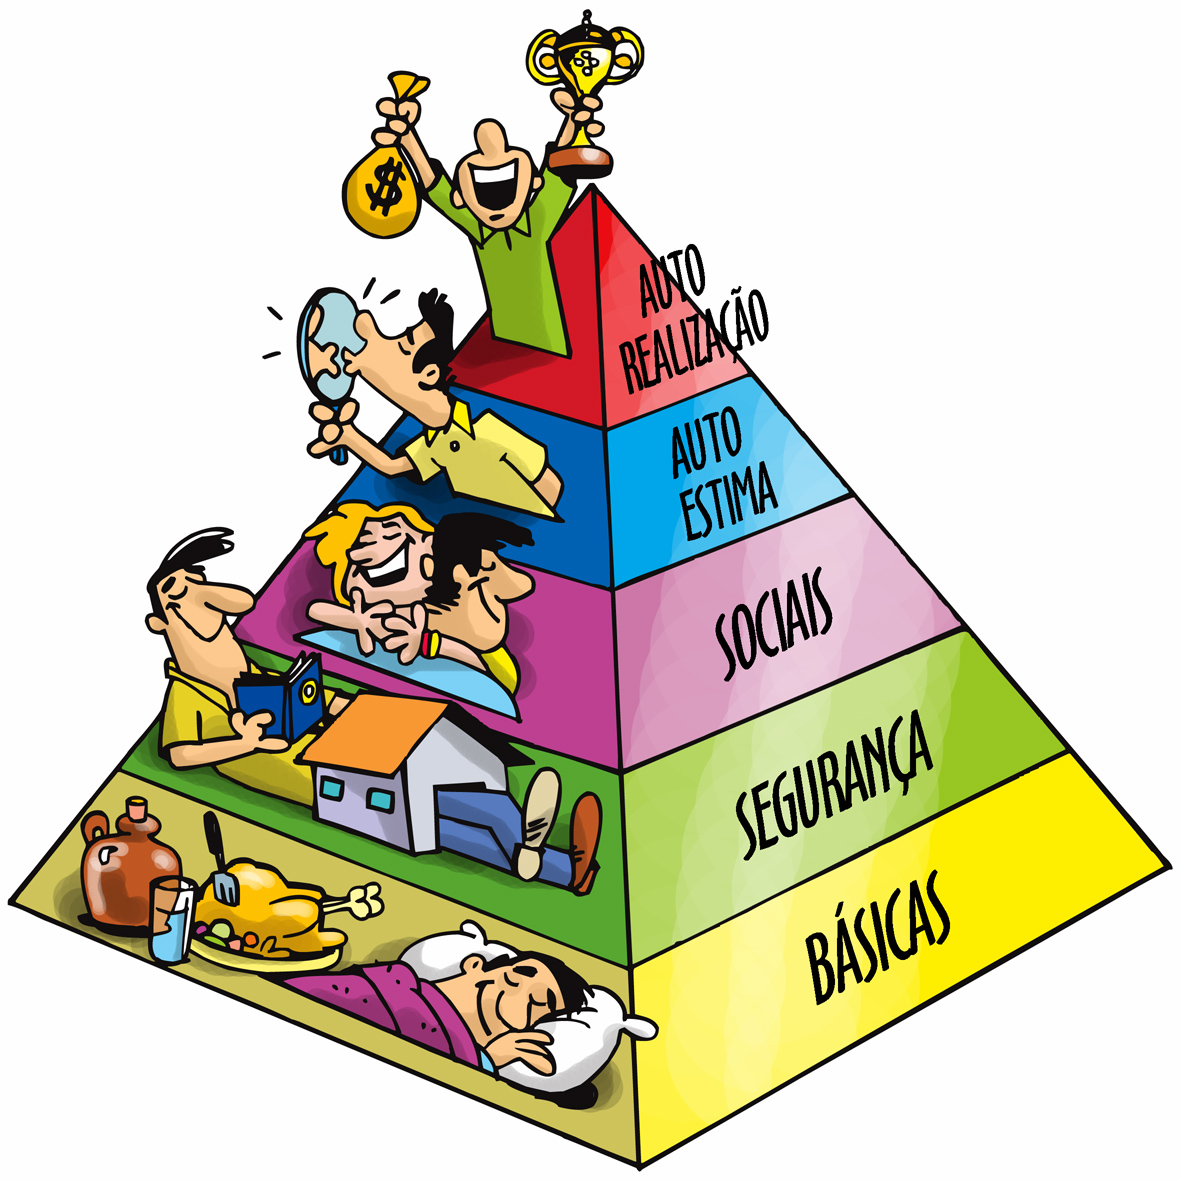
\includegraphics[scale=0.35]{Maslow.jpg}
	\end{center}
	\ABNTEXchapterfont\small{fonte:\href{http://accorh-consultor-wjlemus.blogspot.com.br/2013/10/que-tan-conrrecta-es-la-piramide-de.html}{Pirâmide de Maslow} - acesso em 15.07.2015}
	\label{Maslow}
\end{figure} 
\FloatBarrier
Mas como adquirir segurança? O Relatório do Programa de Desenvolvimento das Nações Unidas de 2014
 usa o antônimo de segurança, ou seja, a vulnerabilidade\footnote{N.A. Veja também em: \href{http://www.ipea.gov.br/portal/index.php?option=com_content&view=article&id=26118&Itemid=383}{Atlas da Vulnerabilidade Social do Brasil} - acesso em 1.9.2015} e faz uma interessante
explanação:
\begin{citacao}
	Uma cobertura que abranja todos os indivíduos pressupõe a necessidade de providenciar serviços
	sociais em diferentes pontos do ciclo de vida, especialmente em períodos sensíveis da vida de uma
	pessoa, incluindo a primeira infância e a transição da adolescência para a juventude e da idade
	adulta para a velhice, a fim de reforçar a resiliência ao longo da vida. É fundamental definir um
	calendário para as intervenções — já que fica dispendioso corrigir mais tarde as consequências da
	falta de apoio ao desenvolvimento de capacidades no momento certo.\cite[p. ~91]{PNUD2014}
\end{citacao}
\par
Os gráficos 1 e 2 melhor definem os
momentos cruciais na infância e ao longo da vida em que é oportuna a intervenção do Estado. O Gráfico 1 sem dúvida é o mais crucial para o caso da tolerância zero, pois a infância e a adolescência são os momentos chaves para a formação do caráter do indivíduo.
\begin{grafico}[h]
	\begin{center}
		\caption{Vulnerabilidades na infância}
		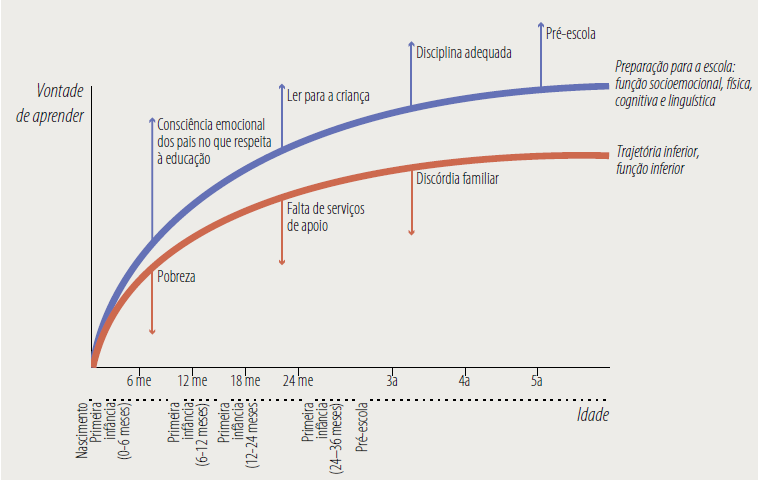
\includegraphics[scale=0.70]{criancap93.png}
	\end{center}
	\ABNTEXchapterfont\small{fonte:\cite[p. ~93]{PNUD2014}}
	\label{Criança}
\end{grafico}
\FloatBarrier
\begin{grafico}[h]
	\begin{center}
		\caption{Vulnerabilidades ao longo da vida}
		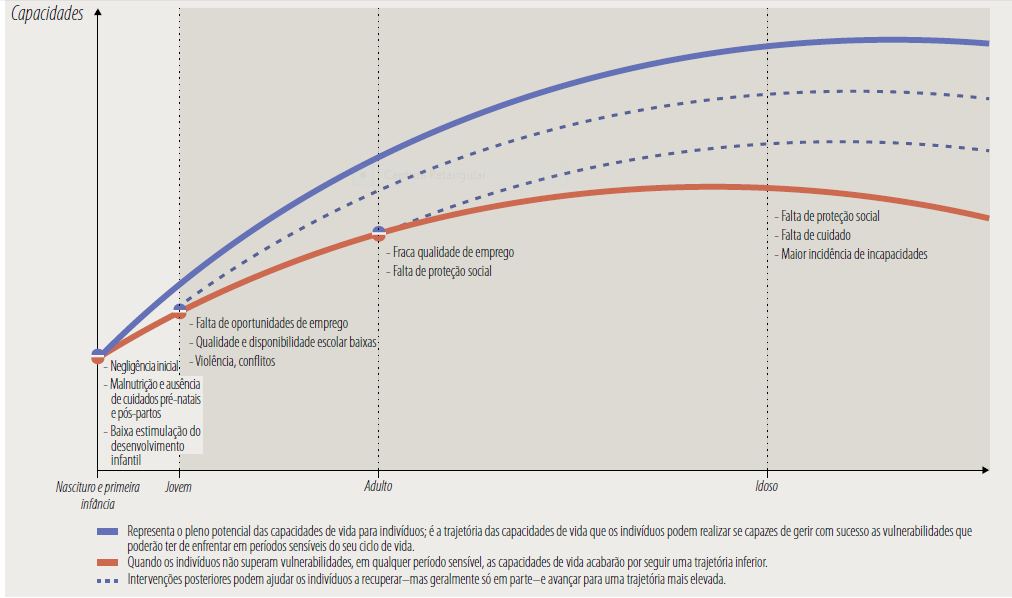
\includegraphics[scale=0.55]{Adultop57.png}
	\end{center}
	\ABNTEXchapterfont\small{fonte:\cite[p. ~57]{PNUD2014}}
	\label{Adulto}
\end{grafico} 
\FloatBarrier
\par
O pesquisador Cláudio Beato\footnote{N.A. Cláudio Beato é sociólogo, coordenador do Centro de Estudos em Criminalidade e Segurança Pública (Crisp) e professor	associado da Universidade Federal de Minas Gerais.} em entrevista a revista \textit{e-metropolis} muito bem revela o que ocorre com a juventude quando o indivíduo está em uma posição de vulnerabilidade:
\begin{citacao}
	Trata-se de um composto de situações, nos quais temos os jovens envolvidos com gangues, a desocupação e a ociosidade
	deles, a baixa disponibilidade dos moradores destes locais em exercer qualquer forma de controle sobre
	o que ocorre com estes jovens até mesmo por medo, bem como as péssimas condições sociais e econômicas ali vigentes.
	O que quero dizer é que há uma lógica nisso. Grupos de jovens que se associam nos bairros; em seguida
	vem a questão da droga e vinculado a ela as armas de fogo, ou seja, de repente, esses grupos de jovens
	estão com armas nas mãos no território onde vivem; e ali já existem disputas que passam a serem vivenciadas de forma mais violenta. Muitas vezes esse jovem é pego pelos instrumentos de controle do estado e acaba indo para a prisão. Lá ocorre um 'upgrade',
	onde estes grupos passam a se estruturar em torno de uma facção criminosa. Vimos isso acontecer com o
	surgimento e crescimento dos grandes grupos como o Comando Vermelho e o PCC. E quando esse jovem sai do sistema prisional, ele leva
	para a sociedade o que foi aprendido ali dentro.\cite[p. ~60]{Beato}
\end{citacao}
\par
De acordo com o acima dito, pode-se definir a evolução para o desvio e a criminalidade da seguinte forma: 
\begin{description}
	\item[fase1] Ociosidade, desocupação, falta de controle dos pais ou da comunidade;
	\item[fase 2] Formação de gangues, uso de drogas, posse de armas, disputas violentas;
	\item[fase 3] Punição pelo Estado, ingresso no sistema prisional, \textit{upgrade} para uma facção criminosa;
	\item[fase 4] Quando sai leva para a sociedade todo o “aprendizado”. 
\end{description}

Rubens Katzman\footnote{Rubens Katzman é diretor de pesquisa sobre integração, pobreza e exclusão social da Universidade Católica do Uruguai} em seu trabalho “Abandonados e Seduzidos” define a segmentação educacional, a segmentação do trabalho e a segregação residencial como causas da vulnerabilidade social: 
\begin{citacao}[spanish]
	\textbf{La segmentación educativa:} La creciente centralidad del conocimiento como instrumento para el progreso de las naciones reafirma el
	papel que se asignó tradicionalmente a la educación	como vía principal de movilidad social y ámbito privilegiado para la integración social de las nuevas generaciones. Ese papel ha sido reiteradamente destacado en los pronunciamientos de las cumbres presidenciales de los últimos años, donde los máximos responsables de las políticas públicas han reconocido que la equidad en los primeros años de vida debe formar parte del núcleo valorativo de los modelos que orientan el desarrollo en América Latina, y que la concentración
	de los recursos de los sistemas educativos en los niños de hogares con bajos niveles socioculturales es uno
	de los medios más eficientes para quebrar los mecanismos de reproducción de la pobreza y de la segmentación social.\\
	\ldots\\ Si los ricos van a colegios de ricos, si la clase media va a colegios de clase media y los pobres a colegios de pobres, parece claro que el sistema educativo	poco puede hacer para promover la integración social y evitar la marginalidad, pese a sus esfuerzos por
	mejorar las oportunidades educativas de los que tienen menos recursos. Por ello es importante destacar no sólo la contribución que el sistema educativo hace a la	equidad por medio de una mayor igualdad en las oportunidades de acceso, sino también su contribución a la
	integración de la sociedad, al crear las condiciones que facilitan la interacción entre desiguales en condiciones de igualdad.\cite[p. ~176-177]{Katzman}
\end{citacao}
\par
\hypertarget{rawls1}{}
Sem dúvida esse é um fato presente nos dias atuais. Ricos estudam em escolas de ricos, a classe média em escolas de classe média e aos pobres resta o ensino público (pelo menos no caso brasileiro). A aplicação do  “princípio da diferença” como definido por John Rawls na definição de \hyperlink{rawls}{Justiça}, pelo menos no ensino fundamental, já faria uma grande diferença, se forem levados em conta os gráficos 1 e 2 acima.

\begin{citacao}[spanish]
\textbf{La segmentación laboral:} Para los efectos del análisis que se desarrolla enseguida, conviene comenzar recordando las observaciones
sintetizadas en el recuadro 1 sobre ciertos aspectos del portafolio de activos de los pobres urbanos que podrían
verse afectados por las transformaciones en el mercado laboral y que tienen incidencia en su grado de aislamiento o de integración en la sociedad:\\
i) Dimensión de capital social individual: el establecimiento donde se trabaja es un lugar privilegiado
para la construcción de redes de amistad, a través de las cuales fluyen recursos en forma de contactos, información y facilidades de acceso a determinados servicios.\\
ii) Dimensión de ciudadanía en sus aspectos subjetivo y objetivo: es también un ámbito privilegiado para la generación de elementos subjetivos de ciudadanía, en el cual se comparten problemas, se consolidan identidades, se afianzan autoestimas y se construye un destino común. Pero también lo es para la adquisición de derechos objetivos de ciudadanía, por medio de conquistas laborales tales como la ampliación y el mejoramiento de las prestaciones sociales usualmente asociadas al rol de trabajador asalariado.\\
iii) Dimensión de capital social colectivo: la participación estable en un mismo establecimiento de trabajadores con distinto grado de calificación aumenta las oportunidades que tienen las categorías de trabajadores menos calificados de acceder a instituciones eficientes en la defensa de sus intereses laborales y en la preservación de derechos ya adquiridos.\cite[p. ~174-745]{Katzman}
\end{citacao}
\par
Tem-se aqui o padrão da maioria das empresas que fazem uso maciço de mão de obra em linhas de montagem, como por exemplo as indústrias automobilísticas: exite uma compartimentação de setores, de competências, \textit{clusters} de funcionários que não se comunicam um com o outro e impedem que alguém de um grupo ascenda ao outro grupo. Não possuem personalidade própria perante a organização e por isso são facilmente substituíveis.
\begin{citacao}[spanish]
\textbf{La segregación residencial} refiere al proceso por el cual la población de las ciudades se va localizando en espacios de composición social homogénea. Entre los factores más importantes que se invocan como antecedentes de estos procesos están el grado de urbanización y la urbanización de la pobreza, el grado de concentración de la distribución del ingreso, las características de la estructura de distancias sociales propias de cada sociedad y la homogeneidad o heterogeneidad de la composición étnica, religiosa o por origen nacional de la población de las ciudades.\cite[p. ~79]{Katzman}
\end{citacao}
\par
Os aglomerados urbanos foram a grande invenção do ser humano, um meio de se proteger e trocar experiências. Quando não existiam os meios de comunicação, ou ainda, quando eram rudimentares, as pessoas interagiam muito mais entre si. Hoje em dia mal cumprimentam seu vizinho. A desigualdade social, as diferenças religiosas, o preconceito de várias formas, estão fazendo as pessoas se isolarem cada vez mais em um espaço que deveria ser usado para interação entre elas.
\par
Os não dotados de um senso minimante humanitário podem argumentar tratar-se do ditado “cada macaco no seu galho”; entretanto esquecem o ditado “quem semeia vento colhe tempestade”. Katzman conclui de forma brilhante:
\begin{citacao}[spanish]
Con todo, estas circunstancias no deberían disuadir la acción sino estimularla, puesto que la alternativa es una
agudización progresiva de la exclusión, con consecuencias imprevisibles para el orden social y la convivencia civilizada. De hecho, esas consecuencias irrumpen tarde o temprano, a veces en forma violenta, anómica e inesperada, a través de los correlatos socialmente
disruptivos de una pobreza marginada por la concentración de privaciones y por su progresivo aislamiento de
las pautas modales de la sociedad. \textbf{La respuesta de las clases medias es apartarse de los lugares y servicios
públicos ocupados por las “clases peligrosas”, cuyos comportamientos, cultivados en el aislamiento y la precariedad generalizada, aparecen a las otras clases como exóticos y desviados}. La deserción de las clases medias
no hace más que acentuar el decaimiento de los espacios públicos, estrechando de ese modo el campo de
experiencias que estimulan la capacidad de empatía con los sectores menos favorecidos y los sentimientos de
obligación moral hacia ellos, y elevando, por ende, el umbral de tolerancia a la desigualdad. La experiencia
acumulada sobre las consecuencias de descuidar estos problemas en las grandes ciudades puede resultar particularmente útil para el diseño de medidas preventivas en las ciudades de tamaño intermedio.\cite[p. ~187, grifo do autor]{Katzman}
\end{citacao}
\par		
Existe um ditado popular no Brasil que
diz “É de pequeno que se desentorta o pepino”, que geralmente é interpretado no sentido punitivo mas deve
sim, ser visto no viés educacional e de prover oportunidades\footnote{N.A. Em um momento em que o Brasil vive uma fase de um quase fanatismo religioso, uma onda de conservadorismo e ainda, para arrepio dos defensores do ECA, veja a passagem bíblica em Eclesiástico 30.7-12}

\section{Do Livre Arbítrio, da Ética, da Moral e da Tolerância}
%\addcontentsline{toc}{section}{Do Livre Arbítrio, da Ética, da Moral e da Tolerância}

\lettrine[lines=2, lhang=0.33, loversize=0.25]{P}{ara} melhor entendimento do presente trabalho, cumpre inicialmente definir como e por que o ser humano age de determinadas maneiras, ora de forma correta, ora de forma errada. O grande diferencial do ser humano dos outros animais sem dúvida é a racionalidade. Então por que certas vezes ele age de forma aparentemente irracional? Por que individualmente ele possui um comportamento manso como uma ovelha e em grupo age como se pertencesse a uma alcateia sem limites??
\par 
Torna-se imperativo descrever brevemente algumas definições basilares inerentes ao comportamento do ser humano enquanto animal e ser racional.
Esses conceitos foram desenvolvidos ao longo da história da humanidade, ora em evidência, ora
caídos ao esquecimento, conforme os regimes políticos foram se alternando na história do mundo.
Por exemplo, durante toda a idade média, o comportamento ético europeu foi ditado pela igreja católica
romana, com as cruzadas, a inquisição e posteriormente pelos reformadores. Um verdadeiro holocausto foi cometido em nome da ética e moral cristã.
\par 
Dessa forma, deve-se partir do comportamento do ser humano individual e paulatinamente introduzir os conceitos de seu comportamento social.
\subsection{Do Livre Arbítrio}
%\addcontentsline{toc}{subsection}{Do Livre Arbítrio}

Foi exatamente no seio da Igreja Católica que Tomás de Aquino desenvolveu seu grandioso trabalho “Suma Teológica” e que nos provê
o primeiro conceito inerente ao ser humano como animal racional e independente, que é o livre arbítrio:
\begin{citacao}
O homem é dotado de livre-arbítrio, do contrário os conselhos, as exortações, os preceitos, as proibições, as recompensas e os castigos seriam vãos. Para demonstrá-lo deve-se considerar  que certas coisas agem sem julgamento. Por exemplo, a pedra que se move para baixo, e igualmente todas as coisas que não tem conhecimento.--Outras coisas agem com julgamento, mas esse não é livre: como os animais. Por exemplo, a ovelha, vendo o lobo, julga que é preciso fugir: é um julgamento natural, mas não livre, pois não julga por comparação, mas por instinto natural. O mesmo acontece com todos os julgamentos dos animais.---O homem, porém, age com julgamento, porque por sua potencia cognoscitiva julga que deve fugir de alguma coisa ou procurá-la. Mas como esse julgamento não é o efeito de um instinto natural aplicado a uma ação particular, mas de uma certa comparação da razão, por isso, o homem age com julgamento livre, podendo se orientar por diversos objetos. . Com efeito, a respeito do contingente, a razão pode seguir direções opostas, como vemos nos silogismos dialéticos e nos argumentos da retórica. Como as ações particulares são contingentes, o julgamento da razão sobre elas se refere  a diversas e não é determinado a uma única. Por conseguinte o homem é dotado de livre-arbítrio, pelo fato mesmo que ser racional.  \cite[p. ~487]{Aquino}
\end{citacao}
\par
Sem dúvida  a existência do livre arbítrio é uma questão controvertida até os dias atuais. Para Aquino é através do livre arbítrio que fazemos nossos julgamentos e nossas escolhas, aceitamos algumas e rejeitamos outras. Isso é um conceito de liberdade. Entretanto existem várias correntes, por exemplo, o Determinismo Radical \citeonline{Klein} \footnote{N.A. Tem-se ainda o Determinismo Liberal e o Determinismo Moderado, mas não serão aqui discutidos} afirma que o livre arbítrio não pode existir pois o homem ao tomar uma ação baseia-se na experiência passada, dessa forma essa não é uma ação livre e portanto a pessoa não pode ser moralmente responsabilizado por ela -- John Locke dizia que o homem ao nascer é uma folha em branco e que adquire conhecimento pela experiência. 
\par
Outros ligam o livre arbítrio ao sentido da responsabilidade, ou seja os atos são (livremente) guiados para 
que seu produto final seja propositadamente um sucesso ou fracasso, para o bem ou para o mal. Poder-se-ia discutir vários outros conceitos, mas independente se o livre arbítrio possui ou não algum nexo causal anterior, para embasar o presente trabalho pressupõe-se que ele existe e que as ações são pautadas única e exclusivamente por uma decisão autônoma do agente. Entretanto a liberdade proporcionada  pelo livre arbítrio vai até onde não prejudica o relacionamento com outras pessoas. A partir daí começam as primeiras restrições, que são dadas pela ética e pela moral.
\subsection{Da Ética e da Moral}
%\addcontentsline{toc}{subsection}{Da Ética e da Moral}

Na sequência deve-se analisar a Ética e a Moral, pois ambas se confundem em muitos casos, além de ser a primeira ação do homem como ser gregário. Uma definição que coaduna com o pensamento do autor deste trabalho pertence a Paul Ricoeur:
\begin{citacao}[english]
	 Though the terms “ethics” and “morality” are often used interchangeably, Ricoeur stipulates a distinction between them. In his usage, ethics deals with the domain of that which is taken to belong to a good human life. It is concerned with the overall aim of a life of action. Morality refers to the expression of this aim in terms of norms that are regarded as somehow obligatory. Moral norms are taken to be universal and to exercise some constraint on conduct. In standard terminology, ethics is teleologically and morality is deontologically oriented. For Ricoeur, these orientations are complementary, not incompatible.
	 At the base of both ethical and moral reflection are two fundamental capabilities described in Ricoeur's anthropology, namely action and imputation. Capable human beings are capable of initiating some new action and what they do is imputable to them as their own freely chosen deed. An event is not an action unless it is imputable to an agent who has a durable identity. Recognition of the imputability of action opens the way for consideration of the ethical and moral determinations of action.\cite{sep-ricoeur}
	\end{citacao}
\par
De acordo com Paul Ricoeur, a ética vem antes da moral e está ligada à liberdade individual. A moral, construída posteriormente, é advinda das leis e normas sociais. Pode-se entender que a ética é o costume de um indivíduo frente às suas escolhas individuais realizadas no exercício de sua liberdade. Já moral é o costume que venceu dentro de um contexto social, tornando-se habitual, um consenso que transforma-se em norma. Algumas normas se expressam em forma de leis, adentrando o campo jurídico.
\par
Nesse sentido jurídico, Nalini nos dá uma interessante definição:

\begin{citacao}
	\textbf{Ética é a ciência do comportamento moral dos homens em sociedade}. É uma ciência, pois
	tem objeto próprio, leis próprias e método próprio, na singela identificação do caráter científico de
	um determinado ramo do conhecimento. O objeto da Ética é a \textbf{moral}. A moral \textbf{é um dos aspectos}
	do comportamento humano. A expressão moral deriva da palavra romana \textit{mores}, com o sentido de
	\textbf{costumes}, conjunto de normas adquiridas pelo uso reiterado de sua pratica.\\
	Com exatidão maior, o objeto da ética é a \textbf{moralidade positiva}, ou seja, 'o conjunto de
	regras de comportamento e formas de vida através das quais tende o homem a realizar o valor do bem'\cite[p. ~19, grifos do autor]{Nalini}
\end{citacao}
\par
Pode-se notar um caráter binário na moral. Se o ato é um costume “do bem” ele é moral, caso contrário será imoral. Não há sustentação para o termo \textbf{amoral}, pois a racionalidade humana não comporta
esse tipo de definição. Dessa forma, pode-se inferir que o ser humano, mesmo ao nascer, já possui uma pequena chama de moral, que de acordo com os costumes de sua cultura, irá ser construída e aprimorada. para o bem ou para o mal.
\par
Ao longo da história o conceito de ética sofreu mudanças.Na era moderna, o conceito de Kant e sua ética do dever era que para ser ético deve ser universalmente aceito; Jurgen Habermas (1989) contradiz Kant em sua ética do discurso e propõe que a ética deve surgir do consenso de diferentes culturas \footnote{N.A. Um exemplo dramático é a mutilação genital feminina em países da África, costume arraigado em algumas populações}(mas pressupõe que todos são iguais no debate) e Enrique Dussel (1995) com a ética da libertação, ou a ética na era da exclusão social (questionando Habermas, pois este não levou em conta as desigualdades sociais). Até mesmo a ciência, que se separou da ética no século XVI através das ideias e descobertas de Galileu, Bacon e Descartes, volta a discutir até onde é ético agir, por conta das descobertas feitas na área nuclear e da biotecnologia.
\par
Como Nalini sugere acima, as normas surgem da reiterada prática de um costume. Por exemplo, o costume de
dizer “bom dia” gerou uma norma de etiqueta social. Como sempre, é uma norma de bem estar social. Quando
uma norma, de forma expressa, pode causar uma sanção para um indivíduo, surge a Lei, que possui uma
definição mais complexa e para solucionar as divergências de sua interpretação surgiu o Direito.
\par
Com as leis pode-se imaginar que a justiça é feita. A lei possui efeitos \textit{erga omnes}, ou seja,
para todos. Mas será que a lei puramente aplicada é justa? A resposta é simples: se assim fosse, não existiriam a doutrina e a jurisprudência.
\par
Uma definição bem mais complexa, do ponto de vista do binômio moral e sociedade é dada pela \textit{Stanford Encyclopedia of Philosophy}
sobre a moralidade. Traz-se aqui alguns excertos do verbete:
\begin{citacao}[english]
	The term 'morality' can be used either
	descriptively to refer to some codes of conduct put forward by a society or, some other group, such as a religion, or
	accepted by an individual for her own behavior or 
	normatively to refer to a code of conduct that, given specified conditions, would be put forward by all rational persons.\\
	\ldots\\
	Descriptive Morality\\
	'Morality' is an unusual word. It is not used very much, at least not without some qualification. People do sometimes talk about Christian morality, Nazi morality, or about the morality of the Greeks, but they seldom talk simply about morality all by itself. Consistent with this way of talking, many anthropologists used to claim that morality, like law, applies only within a society. They claimed that 'morality' refers to that code of conduct that is put forward by a society. However, even in small homogeneous societies that have no written language, distinctions are sometimes made among morality, etiquette, law, and religion. So, even for these anthropologists 'morality' does not often refer to every code of conduct put forward by a society. \\
	\ldots\\
	Normative Morality\\
	The normative sense of 'morality' refers to a universal guide to behavior that, in plausible specified conditions, all rational persons would put forward for governing the behavior of all moral agents. Thus it is important to know what is meant by 'rational person'. In this context, 'rational person' refers to a person insofar as he is acting rationally in the sense described previously. Such a person must have sufficient knowledge and intelligence to understand what kinds of actions morality prohibits, requires, discourages, encourages, and allows, and also must have sufficient volitional ability to use morality as a guide for their behavior. Such rational persons seek to avoid any harm to themselves unless they believe that their action will result in someone, themselves or others, avoiding a comparable harm or gaining a compensating good. People lacking these characteristics are not subject to moral judgment. If they lack them only temporarily, and are not responsible for the lack, they might be excused from moral judgments in those cases. All such rational persons are moral agents.\cite{sep-morality-definition}
	\end{citacao}
\par
Sem dúvida a parte interessante para o presente trabalho é a moralidade normativa. Parte do princípio que toda pessoa \textbf{racional}
em um comportamento social sabe o que é permitido, proibido, encorajado e desencorajado, etc. (possui livre-arbítrio), Dessa forma, pode-se presumir que uma pessoa embriagada é desprovida de moralidade? Pelo acima dito entende-se que sim. Mas a quando a ética e a moral aceitam um flexibilização em sua interpretação, surge a tolerância.

\subsection{Da Tolerância}
%\addcontentsline{toc}{subsection}{Da Tolerância}

Na continuidade deve-se definir a Tolerância e um bom ponto de partida é o conhecido estado de natureza, discutido por vários filósofos, tais como Hobbes, Locke, Rousseau e Voltaire. Segundo o pensamento de Hobbes:
\begin{citacao}
	Num estado de natureza, não existem leis, no verdadeiro sentido da
	palavra. Mas existem «leis da natureza», que tomam a forma de princípios de interesse pessoal racional, de receitas para a maximização
	das possibilidades de sobrevivência. Estas leis levam os homens, no
	seu estado natural, a procurar a paz e a \textbf{prescindir de alguma da sua
	liberdade em troca de iguais concessões por parte dos outros homens}.\cite[p. ~291, grifo do autor]{Kenny}
\end{citacao}
\par
Exatamente essa flexibilização de liberdade é que pode ser caracterizada como tolerância e no caso de Hobbes ela é recíproca. Na interpretação do ponto de vista de Locke:
\begin{citacao}
	Antes de haver estados capazes de promulgar leis, defende Locke,
	os homens têm consciência da existência de uma lei natural, que os
	ensina que todos os homens são iguais e independentes e que ninguém
	deve prejudicar outra pessoa na sua vida, saúde, liberdade ou propriedade. Estes homens, que não têm na Terra ninguém que lhes seja
	superior, encontram-se num estado de liberdade, mas não num estado
	de indisciplina. Além de estarem obrigados pela lei natural, os seres
	humanos possuem direitos naturais, em particular o direito à vida, à
	autodefesa e à liberdade. \textbf{Também têm deveres, em particular o de não
	prescindirem dos seus direitos}.\cite[p. ~293, grifo do autor]{Kenny}
\end{citacao}
\par
Mas as vezes é necessário abrir parcialmente mão de um direito em função de uma convivência harmoniosa, de uma necessidade básica da vida em comunidade e a isso pode-se chamar de tolerância.
\par
Na reunião de 16 de novembro de 1995, a Organização das Nações Unidas para a Educação, Saúde e Cultura - UNESCO, por ocasião da 28\textordfeminine Reunião da Conferência Geral, publicou a “Declaração dos Princípios sobre a Tolerância”\footnote{N.A. - Traduzida para o portugês em 1997 pela Universidade de São Paulo}, de onde se destaca:
\begin{citacao}
	\textbf{Artigo 1\textordmasculine - Significado da Tolerância} \\
		1.1 A tolerância é o respeito, a aceitação e o apreço da riqueza e da diversidade das culturas de nosso mundo, de nossos modos de expressão e de nossas maneiras de exprimir nossa qualidade de seres humanos. É fomentada pelo conhecimento, a abertura de espírito, a comunicação e a liberdade de pensamento, de consciências e de crença. A tolerância é a harmonia na diferença. Não é só um dever de ordem ética; é igualmente uma necessidade política e jurídica. A tolerância é uma virtude que torna a paz possível e contribui para substituir uma cultura de guerra por uma cultura de paz.\\
		1.2 \textbf{A tolerância não é concessão, condescendência, indulgência}. A tolerância é, antes de tudo, uma atitude fundada no reconhecimento dos direitos universais da pessoa humana e das liberdades fundamentais do outro. Em nenhum caso a tolerância poderia ser invocada para justificar lesões a esses valores fundamentais. A tolerância deve ser praticada pelos indivíduos, pelos grupos e pelo Estado.\\
		1.3 A tolerância é o sustentáculo dos direitos humanos, do pluralismo (inclusive o pluralismo cultural), da democracia e do Estado de Direito. Implica a rejeição do dogmatismo e do absolutismo e fortalece as normas enunciadas nos instrumentos internacionais relativos aos direitos humanos. \\
		1.4 Em consonância ao respeito dos direitos humanos, \textbf{praticar a tolerância não significa tolerar a injustiça social, nem renunciar às suas próprias convicções, nem fazer concessões a respeito}. A prática da tolerância significa que toda pessoa tem a livre escolha de suas convicções e aceita que o outro desfrute da mesma liberdade.Significa aceitar o fato de que os seres humanos, que se caracterizam naturalmente pela diversidade de seu aspecto físico, de sua situação, de seu modo de expressar-se, de seus comportamentos e de seus valores, tem o direito de viver em paz e de ser tais como são. Significa também que ninguém deve impor a sua opinião a outrem. \\
	\textbf{Artigo 2\textordmasculine -  O papel do Estado}\\
		2.1 No âmbito do Estado a tolerância exige justiça e imparcialidade na legislação, na aplicação da lei e no exercício dos poderes judiciário e administrativo. Exige também que todos possam desfrutar de oportunidades econômicas e sociais sem nenhuma discriminação. \textbf{A exclusão e a marginalização podem conduzir à frustração, à hostilidade e ao fanatismo}.\cite[p. ~11-12, grifos do autor]{Une}
\end{citacao}
Note-se que no subitem 1.2 que a tolerância não seve ser um sinônimo de aceitação de desvios que porventura venham a prejudicar a si ou outras pessoas. A prática reiterada e não punida de algum delito pode causar um aparente sentimento de tolerância nas pessoas, causado pela desilusão de não ver a justiça ser feita. Tudo o que foi acima dito, pode agora ser resumido nas definições de Max Weber a seguir.

\section{Da Ação Social, Relação Social, Poder e suas variações}
%\addcontentsline{toc}{section}{Da Ação Social, Relação Social, Poder e Dominação}

\lettrine[lines=2, lhang=0.33, loversize=0.25]{P}{ara} melhor contextualizar a “morality” exercida em sociedade, tal como definida pela \textit {Stanford Encyclopedia of Philosophy}, torna-se primordial trazer à colação conceitos fundamentais definidos por Max Weber
em seu livro “Economia e Sociedade”, também pertinentes ao escopo do presente trabalho:
\paragraph*{\textbf{Da Ação Social}}

\begin{citacao}
	A ação social, como toda ação, pode ser determinada: 1)\textit{de modo racional referente a fins}: por expectativas quanto ao
	comportamento de objetos do mundo exterior e de outras pessoas, utilizando essas expectativas como “condições” ou “meios” para alcançar
	fins próprios, ponderados e perseguidos racionalmente, como sucesso; 2)\textit{de modo racional referente a valores}: pela crença
	consciente no valor -- ético, estético, religioso ou qualquer que seja a sua interpretação --- absoluto e \textit{inerente} a determinado
	comportamento como tal, independentemente do resultado; 3)\textit{de modo afetivo} especialmente \textit{emocional}: por afetos ou
	estados emocionais atuais; 4)\textit{de modo tradicional}:por costume arraigado.\cite[p. ~15]{Weber}
\end{citacao}
\par
Quando Weber menciona a ação referente a fins pressupões que a pessoa busca através da ação social coisas que o beneficiem; quanto aos valores, busca determinados comportamentos seja de forma moral, religiosa, etc; o modo afetivo pode ser interpretado como ser bem quisto por seus amigos e familiares e, de modo tradicional pela aceitação da cultura de seu meio.
\paragraph*{\textbf{Da Relação Social}}
\begin{citacao}
	Uma relação social denomina-se “relação comunitária” quando e na medida que a atitude na ação social -- no caso particular ou em média
	ou no tipo puro -- repousa no sentimento subjetivo  dos participantes de pertencer (afetiva ou tradicionalmente) ao mesmo grupo.\\
	Uma relação social denomina-se “relação associativa” quando e na medida em que a atitude na ação social repousa num ajuste ou numa união de interesses racionalmente motivados (com referência a valores ou fins). A relação associativa, como caso típico, pode repousar especialmente (mas não unicamente) num acordo racional, por declaração recíproca. Então a ação correspondente quando é racional, está orientada: a) de maneira racional referente a valores, pela crença no compromisso próprio; b) de maneira racional referente a fins pela expectativa de lealdade da outra parte.\cite[p. ~25]{Weber}
	\end{citacao}
\par
Aqui pode-se entender que na relação comunitária, a pessoa necessita fazer parte de um ou alguns determinados grupos (grupo familiar por exemplo); na associativa pode-se entender como a pessoa pertencente a um determinado grupo religioso, uma associação de bairros, etc.
\hypertarget{poder}{}
\paragraph*{\textbf{Do Poder e suas variações}}
\begin{citacao}
	Poder significa toda probabilidade de impor a própria vontade numa relação social, mesmo contra resistências, seja qual for o fundamento dessa probabilidade.\hyperlink{S2}{Ver Análise SWOT}\\
	Dominação é a probabilidade de encontrar obediência a uma ordem de determinado conteúdo, entre determinadas pessoas indicáveis; disciplina
	é a probabilidade de encontrar obediência pronta, automática e esquemática a uma ordem, entre uma pluralidade indicavel de pessoas, em virtude de atividades treinadas.\cite[p. ~33]{Weber}
\end{citacao}
\par
Sem dúvida é a mais forte das definições de Weber e a maneira mais fácil é através de exemplos: para poder, um regime ditatorial é o exemplo do uso da ameaça e da força para impor a vontade; a dominação é o que uma facção criminosa faz em uma comunidade e a disciplina é o regime adotado nos quarteis.
\par
Essas definições serão devidamente expandidas e/ou correlacionadas quando da análise SWOT e nas Considerações adicionais.
\paragraph*{\textbf{Outras considerações}}
O potiguar Gaudêncio Torquato\footnote{N.A. Jornalista, consultor de marketing institucional e político, consultor de comunicação organizacional, doutor, livre-docente e professor titular da Universidade de São Paulo e diretor-presidente da GT Marketing e Comunicação} em sua coluna semanal no jornal jurídico eletrônico Migalhas criou uma “versão brasileira” da ação social e fez uma interessante definição sobre como agem as pessoas:
\begin{citacao}
	As pessoas agem de acordo com quatro instintos ou impulsos. O primeiro é o \textbf{instinto combativo}, a necessidade de preservar-se, viver bem ; daí a luta contra as intempéries, os adversários, tudo que seja ameaça à sobrevivência. Se o Estado não lhe dá garantia de uma vida saudável, que vá pro inferno, sugere mentalmente. O segundo é \textbf{o instinto alimentar}, a necessidade de garantir o estômago para sobreviver. Na luta contra a fome, contra a miséria, recorre igualmente ao Estado. Daí o medo do desemprego, da falta de dinheiro. O terceiro é o \textbf{impulso sexual}, que garante a preservação da espécie ; e o quarto, o \textbf{instinto paternal}, é o responsável pelos vínculos da solidariedade, do amor à família, do carinho, da amizade, do companheirismo. Uma crise nos dois primeiros sistemas afeta os dois últimos, amortecendo os valores espirituais. Se não se sentem protegidas, as massas acabam se voltando contra os dirigentes que prometeram protegê-las.\cite{Migalhas} 
\end{citacao}
\par
Sem dúvida as definições acima podem muito bem complementar as de Weber, e ainda nota-se que as ações são bem peculiares ao povo brasileiro.
\par
Encerra-se aqui a definição de parte dos conceitos que regem o ser humano tanto individualmente como socialmente. Entretanto, um ultimo conceito deve ser abordado, com consequências diretas sobre as ações do homem em uma sociedade, que é a justiça.

\section{Da Justiça}
%\addcontentsline{toc}{section}{Da Justiça}

\lettrine[lines=2, lhang=0.33, loversize=0.25]{I}{ncontáveis} autores criaram definições sobre justiça. Deve-se imaginar que até o leitor do presente trabalho tenha a sua em particular. Mas vale destacar três notáveis:
\par
Inicialmente o conceito do que é justo, ou o que é justiça na visão de
Norberto Bobbio (2007) que a define como:

\begin{citacao}
	I - UM CONCEITO NORMATIVO --- A justiça é um fim social, da mesma forma que a igualdade ou a liberdade ou a democracia ou o bem estar. Mas há uma diferença importante  entre o conceito de Justiça e os outros citados. Igualdade, liberdade, etc. são termos descritivos. Embora abstratos e teóricos podem ser definidos de tal modo que as afirmações em que se evidenciam são verificáveis, de um modo geral, pelo simples confronto com a evidência empírica.\\
	\ldots \\
	II. DEFINIÇÃO --- Se a justiça é um conceito normativo, surge agora o problema da possibilidade de a definir em termos descritivos. A Justiça foi equiparada à legalidade , à imparcialidade, ao igualitarismo, e à retribuição do indivíduo segundo seu grau, sua habilidade ou sua necessidade, etc. Ora, se estas definições fossem aceitáveis, poderíamos partir de premissas baseadas em fatos para chegar a conclusões normativas. Por exemplo, se “justo” tiver o mesmo significado de “igual” e, portanto, se uma determinada norma for igualitária, concluiremos logicamente que ela também é justa. Logicamente seria por isso incoerente para qualquer um considerar injustas tanto as normas igualitárias como as normas não-igualitárias.Evidentemente que estas definições não são aceitáveis. Evidentemente que não podemos ir do “ser” para o “dever ser” e dos fatos para os valores. Todas as definições de Justiça aqui apresentadas não são, de fato, definições e sim juízos normativos, sob a capa verbal de definições, tendo como finalidade geral uma eficácia retórica. Por esse motivo, afirmações como “a Justiça significa igualitarismo” devem ser interpretadas, não como uma definição do conceito de Justiça, mas como expressão do princípio normativo de que as normas igualitárias de distribuição são justas e as não-igualitárias injustas, de onde se concluiria que apenas as normas do primeiro tipo deveriam ser aprovadas e aplicadas. \textbf{A melhor coisa é considerar a Justiça como noção ética fundamental e não determinada}.\cite[p. ~660, grifo do autor]{Bobbio2007}
\end{citacao}
\par
Essa visão de Bobbio sem dúvida é a mais voltada à área jurídica de todas aqui apresentadas. Será usada no sentido de “norma igualitária” mais adiante nas Considerações adicionais.
\par
Ruy Barbosa em sua “Oração aos Moços”\footnote{Esse texto de Rui Barbosa foi lido por ocasião da formatura da turma de 1921 da Faculdade de Direito do Largo São Francisco em São Paulo - SP. O autor, que foi o paraninfo da turma, não pode comparecer por estar adoecido.}  utiliza os conceitos de Aristóteles e Tomás de Aquino de justiça, que definem o conceito de igualdade para os desiguais, sob a ótica da justiça:

\begin{citacao}
	\textbf{A regra da igualdade não consiste senão em quinhoar desigualmente aos desiguais, na medida em que se desigualam}. Nesta desigualdade social, proporcionada à desigualdade natural, é que se acha
	a verdadeira lei da igualdade. O mais são desvarios da inveja, do orgulho, ou da loucura. Tratar com desigualdade a iguais, ou a desiguais com igualdade, seria desigualdade flagrante, e não igualdade
	real. Os apetites humanos conceberam inverter a norma universal	da criação, pretendendo, não dar a cada um, na razão do que vale, mas atribuir o mesmo a todos, como se todos se equivalessem.
	Esta blasfêmia contra a razão e a fé, contra a civilização e a humanidade, é a filosofia da miséria, proclamada em nome dos direitos do trabalho; e, executada, não faria senão inaugurar, em vez da
	supremacia do trabalho, a organização da miséria. Mas, se a sociedade não pode igualar os que a natureza criou 	desiguais, cada um, nos limites da sua energia moral, pode reagir 	sobre as desigualdades nativas, pela educação, atividade e perseverança. \cite[p. ~26, grifo do autor]{Rui}
\end{citacao}
\par
Há quase 100 anos, Rui Barbosa já colocava um princípio da igualdade em termos da desigualdade social. Mais radical ainda, complexa, porém completa é a definição de justiça de John Rawls  conforme segue:
\begin{citacao}
	Os princípios da justiça são escolhidos por trás de um véu de ignorância. Isso garante que ninguém seja favorecido ou desfavorecido na escolha dos princípios pelo resultado do acaso natural ou pela contingencia de circunstâncias sociais. Uma vez que todos estão numa situação semelhante e ninguém pode propor princípios que favoreçam sua própria situação, os princípios da justiça são o resultado de um acordo ou pacto justo. Dadas as circunstancias da posição original, a simetria das relações de todos para com todos os demais, essa situação original e equitativa entre os indivíduos tidos como pessoas morais\footnote{N.A.:na segunda edição desse livro é usado o termo 'éticos'}, isto é, como seres racionais com objetivos próprios e capazes, presumirei, para ter um senso de justiça.\cite[p. ~15]{Rawls}\\
\end{citacao}
\par
Não é objeto desse trabalho traçar todas as considerações que Rawls faz para justificar seus princípios de justiça, mas entende-se necessário explicitar melhor a Posição Original e o Véu da Ignorância, conforme Denis Coitinho assim explica:
\begin{citacao}
	\textbf{Posição original/véu da ignorância:} experimento mental usado por John Rawls que representa uma situação de escolha que é realizada sob certas circunstâncias. Substitui o “estado da natureza” utilizado nas teorias modernas do contrato social. As circunstâncias da escolha são as (i) da justiça, uma vez que pressupões escassez moderada de recursos e que as pessoas sejam minimante morais e as (ii) do véu da ignorância, uma vez que essa escolha será realizada sem conhecimento particular do que constitui um bem para os indivíduos. As partes apenas desejam os bens primários, como direito, liberdade, renda, riqueza e autoestima. Dadas essas circunstâncias, e levando em conta os princípios alternativos do utilitarismo, kantismo e perfeccionismo, seria razoável e racional escolher os princípios de igual liberdade, igualdade equitativa de oportunidade e o princípio da diferença para regrar as principais instituições políticas e econômicas da sociedade.\cite[p. ~303]{Coitinho}
\end{citacao}
\par
Após essas considerações, pode-se partir finalmente para os princípios definidos por Rawls:
\begin{citacao}
	\textbf{\textit{Primeiro princípio}}\\
	Cada pessoa deve ter um direito igual ao mais abrangente sistema total de liberdades básicas iguais que seja compatível com um sistema similar de liberdades para todos.\\\\
	\hypertarget{rawls}{}
	\textbf{\textit{Segundo princípio}}\\
	As desigualdades econômicas e sociais devem ser dispostas de modo a que tanto:\\
	(a) se estabeleçam para o máximo benefício possível dos menos favorecidos que seja compatível com as restrições do princípio de poupança justa, como\\
	(b) estejam vinculadas a cargos e posições abertos a todos em condições de igualdade equitativa de oportunidades. \hyperlink{rawls1}{voltar para Katzman}\\
	\textbf{\textit{Primeira regra de prioridade}} (a prioridade da liberdade)\\
	Os princípio de justiça devem ser dispostos em ordem lexical e, portanto, só se podem restringir as liberdades básicas em nome da própria liberdade. Existem dois casos:\\
	(a) uma liberdade menos extensa deve fortalecer o sistema total de liberdades partilhado por todos;\\
	(b) uma liberdade desigual deve ser aceitável para aqueles que tem menor liberdade.\\
	\textbf{\textit{Segunda regra de prioridade}} (a prioridade da justiça sobre a eficiência e o bem estar)\\
	O segundo princípio de justiça precede lexicalmente o princípio da eficiência e o princípio da maximização da soma de vantagens; e igualdade equitativa de oportunidades precede o princípio de diferença. Há dois casos:\\
	(a) a desigualdade de oportunidades deve aumentar as oportunidades daqueles que tem menos oportunidades;\\
	(b)uma taxa elevada de poupança deve, pesando-se tudo, mitigar o ônus daqueles que carregam esse fardo.\cite[p ~376]{Rawls}
\end{citacao}
\par
Sem dúvida o mais controvertido dos princípios é o da diferença (segunda regra de prioridade, letra \textit{a}) onde se entende que uma distribuição desigual será justa, se e somente se o resultado global de tal desvio beneficiar aqueles membros da sociedade que são proporcionalmente menos favorecidos, em conceder-lhes mais do que receberiam em uma distribuição igualitária.
\par
Outro fato interessante é o “crescendo” em termos sociais nas interpretações de Bobbio, passando por Rui Barbosa e finalizando em Rawls. Enquanto o primeiro possui uma visão legalista de justiça (Bobbio é o filósofo predileto dos acadêmicos de direito), Rui Barbosa ameniza e propõe uma distribuição desigual; Rawls também a admite desde que favoreça ainda mais os desfavorecidos.
\par
Rawls formulou sua teoria em 1972 e apenas dois anos depois, seu próprio colega em Harvard, Robert Nozik, publicou um livro
chamado “Anarquia, Estado e Utopia” e ainda, em 1976, Frederick Hayek em seu livro “A Miragem da Justiça Social”, criticaram os
princípios de Rawls, pregando a intervenção mínima do Estado em todas as áreas e a liberdade de agir inclusive para o capital. 
\par
Era o surgimento do modelo neoliberal do Estado, implantado profundamente nos governos Tatcher (Inglaterra) e Reagan (EUA) na década de 1980, com consequências funestas até os dias atuais, segundo vivencia do autor. Desemprego, privatizações, entrega de bens do estado ao capital a preços irrisórios (no caso Brasileiro a Cia. Vale do Rio Doce), a total falta de respeito com o ser humano, a implantação do modelo gerencial do Estado e o cidadão tratado como cliente\footnote{N.A. Cliente é aquele que paga para usufruir de um serviço} Essas foram as heranças do neoliberalismo. À essa época uma bem humorada sátira circulou na Inglaterra como mostra a figura 2.
\begin{figure}[!htpb]
	\caption{\label{Figuraa}E o vento levou...}
	\begin{center}
		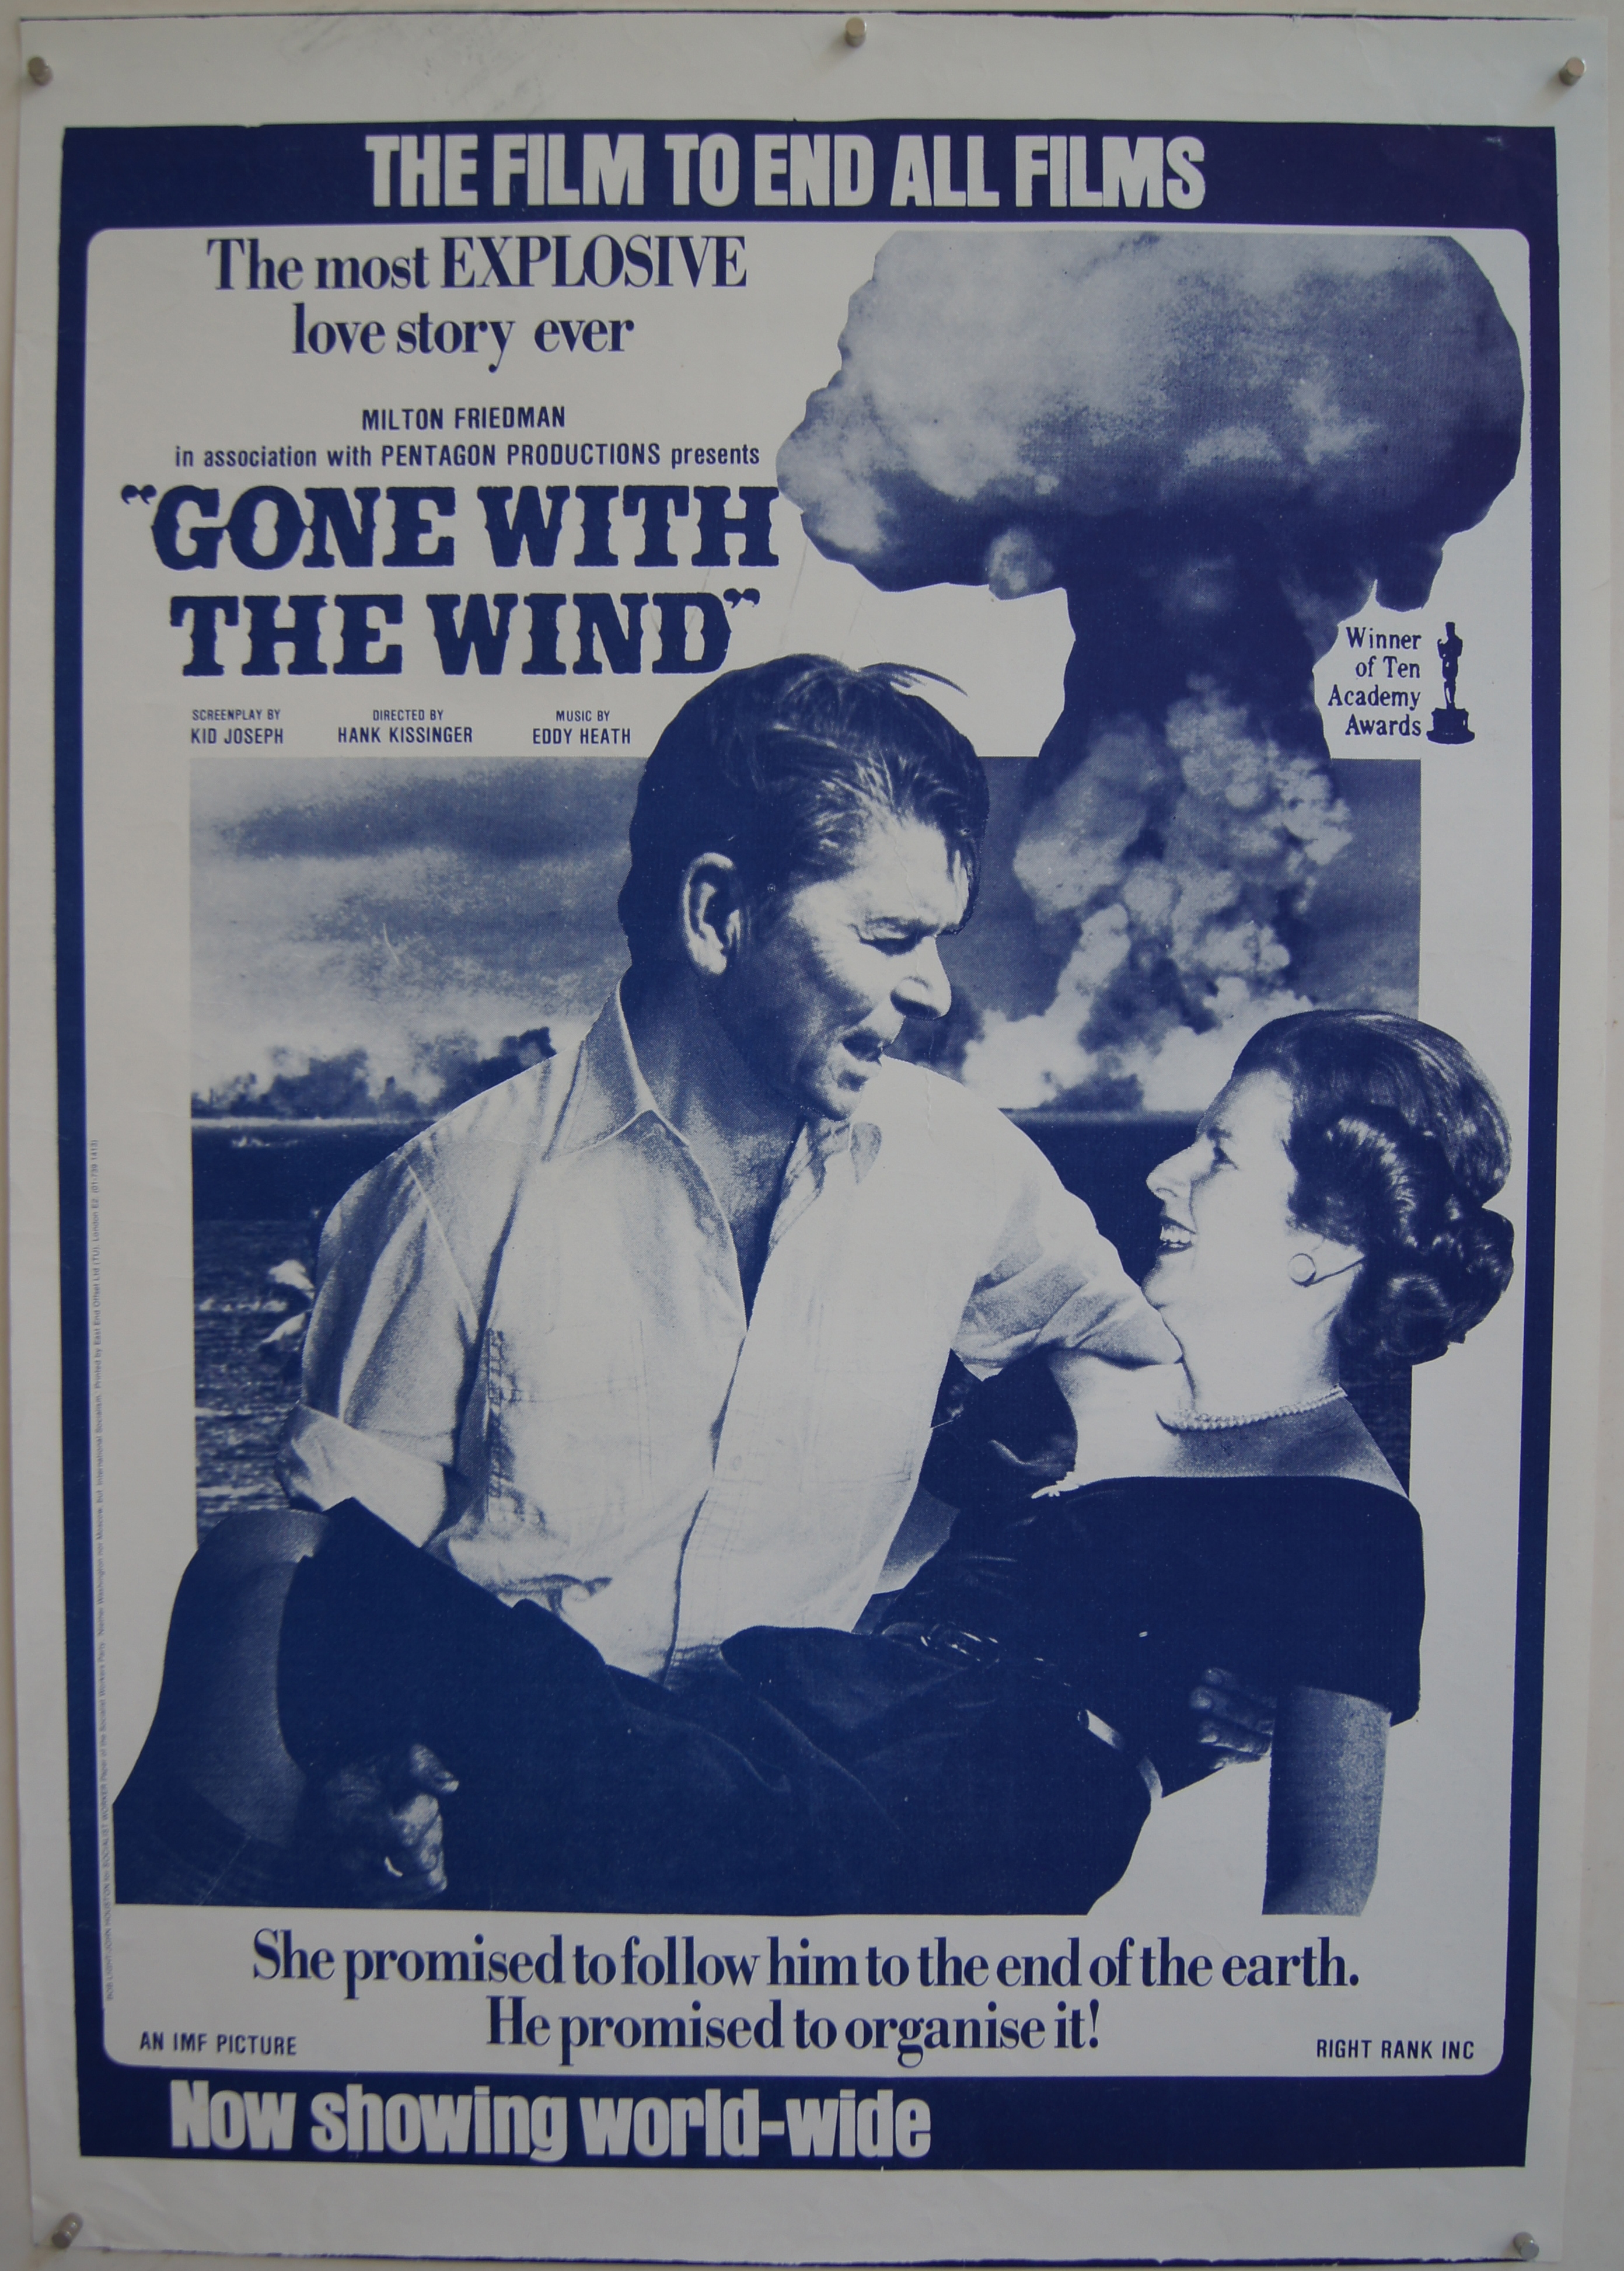
\includegraphics[scale=0.14]{ventolevou.jpg}
	\end{center}
	\ABNTEXchapterfont\small{fonte:Acervo do autor - 1986}
\end{figure}
\FloatBarrier
\par
Do acima dito, pode-se concluir que em uma ambiente liberal, com domínio pelo capital, nunca ter-se-á a justiça de forma plena e muito menos \href{http://www.bbc.com/portuguese/noticias/2015/09/150923_vw_escandalo_cc}{honestidade} visto os interesses envolvidos serem inconfessáveis. Para isso, entende-se que somente com um estado de bem estar social implantado, nos moldes preconizados por Keynes, Rawls e ainda com as concepções de Angus Deaton (prêmio Nobel de economia em 2015), a justiça seria plenamente possível entre os desiguais. 
\par
Entretanto, não se deve afastar de imediato as ideias de Nozick e Hayek mas sim ponderar e discuti-las de forma a encontrar um ponto de equilíbrio  entre eles e Rawls.
\par
Nosso país ainda é muito conhecido pelo “jeitinho brasileiro” e ele ainda prevalece (veja a questão 48 do questionário no Anexo A) ou ainda a “Lei de Gérson”\footnote{N.A. A Lei de Gérson nasceu  na década de 1970 a partir da propaganda de uma marca de cigarros em que o ex jogador da seleção brasileira de futebol (Gérson) dizia “Por que pagar mais caro se o Vila me dá tudo aquilo que eu quero de um bom cigarro? Gosto de levar vantagem em tudo, certo? Leve vantagem você também, leve Vila Rica!”. Essa frase emblemática transformou-se na definição de uma pessoa que sempre leva vantagem, independente de valores éticos ou morais.} e outros tantos termos pejorativos pelos quais nossa população é conhecida. A corrupção é cultural em nosso país e os jornais a denunciam quase diariamente, o famoso “171” (estelionato no nosso Código Penal) é um termo corriqueiro aqui e muitos se orgulham em utilizá-lo para descrever suas proezas de moral duvidosa.
\par
Outros conceitos serão mostrados doravante, mas entende-se que os basilares para nortear a compreensão do presente trabalho foram aqui apresentados. Cumpre agora, paulatinamente, partir para a parte prática do presente trabalho.

% ----------------------------------------------------------
\chapter{A teoria das Janelas Quebradas e a Política de Tolerância Zero}
\section{Origem, Prós e Contras}

\lettrine[lines=2, lhang=0.33, loversize=0.25]{E}{m} 1969 o psicólogo Philip Zimbardo\footnote{N.A. Philip Zimbardo é um polêmico professor na Universidade de Stanford - USA que ficou famoso ao fazer um experimento que simulava uma prisão dentro da Universidade usando seus próprios alunos como atores com consequências quase fatais \href{http://www.prisonexp.org/portuguese-1/}{(Prisão em Stanford)}. Em 2003 ganhou o premio IgNobel de psicologia por seu trabalho “Politicians Uniquely Simple Personalities” \href{http://www.improbable.com/ig/ig-pastwinners.html\#ig2003}{Prêmio IgNobel 2003}. Sua última obra é o livro “O Efeito Lúcifer: Entendendo como pessoas boas se tornam diabólicas”.} relatou um experimento em que colocou 2 automóveis idênticos (mesmo modelo, cor, ano e sem identificação) no bairro do Bronx em New York, bairro conhecido pelo alto índice de violência, sujeira e descumprimento das leis e outro em Palo Alto, Califórnia, local de alto nível cultural e alta conscientização de cidadania, ambos sob a atenta observação de psicólogos.
\par
O carro do Bronx em poucas horas começou a ser vandalizado, levaram as rodas, radiador, motor, radio, enfim, tudo o que pudesse ser aproveitado. A carcaça que sobrou virou uma espécie de \textit{play-ground} para as crianças.
\par
Passada uma semana, o carro deixado em Palo Alto mantinha-se intacto, sem nenhum sinal de vandalismo. Foi quando um dos pesquisadores foi até o carro e quebrou o vidro de uma de suas janelas. A consequência foi imediata: o carro começou a ser vandalizado da mesma forma que o do Bronx, por pessoas que teoricamente possuem um alto grau de cidadania.
\par
A conclusão que os psicólogos chegaram foi que independente do nível social, cultural e financeiro, quando se apresenta uma situação de descaso, de desordem para com um determinado bem ou mesmo uma determinada região, é gerada suposição que ali não existe controle pelas autoridades, é uma terra de ninguém onde tudo é permitido\footnote{N.A. Esse conceito será utilizado pelo autor em outras passagens do texto e para sintetizá-lo foi denominado \textbf{paradigma de Zimbardo.}}.
\par
\begin{foto}[!htpb]
	\caption{\label{Foto0}O “paradigma de Zimbardo” em Natal - Antigo Hotel Reis Magos}
	\begin{center}
		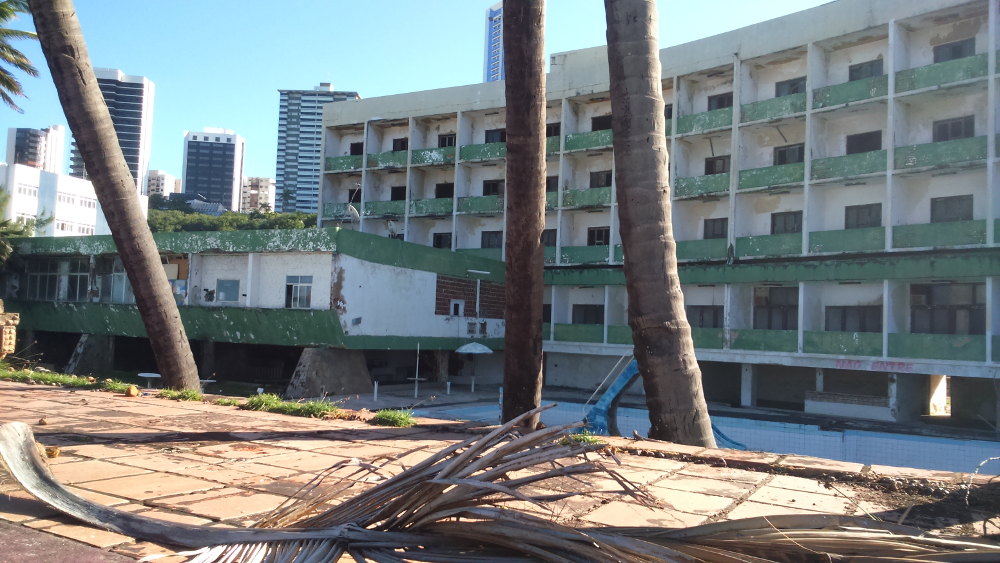
\includegraphics[scale=0.45]{reis_magos2.png}
	\end{center}
	\ABNTEXchapterfont\small{Fonte: Produzida pelo autor - agosto de 2015}
\end{foto}
E mais, na medida em que as infrações vão ocorrendo sem punição, chega-se a um nível exponencial de degradação onde é praticamente impossível retomar o controle.
\par
Um exemplo do descaso do poder público (por poder público entenda-se legislativo, executivo e judiciário) é o antigo prédio do Hotel Reis Magos
mostrado na Foto 1. Até quando vai durar a queda de braço entre preservacionistas e vanguardistas? O proprietário está calmamente de braços cruzados esperando o prédio ruir. Enquanto isso, o lugar virou um ponto de consumo de drogas e pernoite para sem-tetos. No momento da presente foto o autor notou um alegre churrasco entre amigos sob as ruínas.
\par
Mas a Teoria das Janelas Quebradas começou verdadeiramente a ser desenvolvida por James Q. Wilson, cientista político e George Kelling, psicólogo criminologista quando publicaram um artigo na Atlantic Monthly, estabelecendo pela primeira vez uma relação de causalidade entre desordem e criminalidade.
\par
Os autores utilizaram o exemplo que se alguém quebra uma janela de um prédio e ninguém a conserta, em breve todas as outras também serão quebradas. O mesmo ocorre quando se estaciona em local proibido, joga lixo na rua, prostituição, jogo do bicho, etc. ou seja, coisas que se pode classificar como
contravenções penais, na verdade está se abrindo espaço para que o crime organizado também se instale naquele local(paradigma de Zimbardo).
\par
Esse tipo de relação pode ser facilmente exemplificado no Brasil na cidade do Rio de Janeiro (Foto 2), onde os morros são dominados por facções ligadas ao tráfico de drogas e onde até alguns anos atrás as condições de vida nessas regiões eram extremamente precárias pela falta de infraestrutura, sujeira e miséria.
\begin{foto}[!htpb]
	\caption{\label{Fotoa}Favela no Rio de Janeiro - RJ}
    \begin{center}
    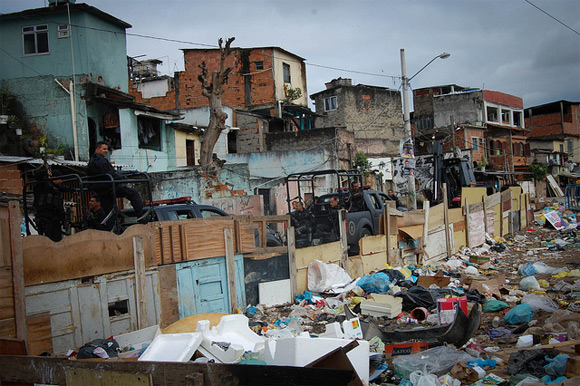
\includegraphics[scale=0.8]{FavelaRJ.jpg}
    \end{center}
    \ABNTEXchapterfont\small{fonte:\href{http://abordagempolicial.com/wp-content/uploads/2012/10/Ocupação-de-Favelas-no-Rio-de-Janeiro-UPP-4.jpg}{Favela no Rio de Janeiro} - acesso em 27.5.2015}
\end{foto}
\par
Vários outros experimentos foram feitos para constatar essa relação de causalidade, como por exemplo
em um estacionamento de supermercado foram colocadas placas pedindo aos clientes que devolvessem os
carrinhos nos locais adequados, entretanto alguns foram deliberadamente deixados aleatoriamente
espalhados no estacionamento. O resultado foi que após poucas horas o número de carrinhos espalhados  no local aumentou de forma exponencial.
\par
O mesmo aconteceu com “não jogue lixo aqui” com um pouco de lixo deixado propositadamente no local e as pessoas passaram a jogar mais lixo,
dentre vários outros experimentos foram feitos para comprovar a teoria. Em síntese, tudo leva a crer que
quando uma desobediência inicial sinaliza para uma ausência de coerção, a anarquia está pronta para ser
instalada. Não se trata de combater a pessoa, mas sim o delito.
\par
Os criadores da Broken Windows Theory definiram desordem como:
\begin{citacao}[english]
	What is disorder? In its broadest  social sense, disorder is incivility, boorish and threatening behavior that disturbs life, especially disturbs urban life.Urban life is characterized  by the presence of many strangers, and in such circunstances citizens need minimum
	levels of order.\cite[p. ~14]{Kelling}\\
	\ldots\\
	By disorder we refer specifically to aggressive panhandling, street prostitution, drunkenness and public drinking, menacing behavior,
	harassment, obstruction of strrets and public spaces, vandalism and graffiti, public urination and defecation, unlicensed  vending
	and paddling, unsolicited window washing cars (“squeegeeing”), and other such acts. While many of these behaviors are designated as criminal, they are usually classified as misdemeanors or petty offenses under state laws and city ordinances, mos often punishable only by fines or community service.\cite[p. ~15]{Kelling}\\
	\ldots\\
	When are disorderly acts really serious? At what point does their seriousness merit intervention? Why should some person engaging in disorders behaviors be warned and/or arrested, and no others? The answers to these questions require a determination based upon two measures: first, the seriousness virtually any crimen -- major as well as minor -- is determined not solely by the heinouness of the act itself, but also by the context in which the behavior takes place. Second, the seriousness of any crime is similarly dependent not upon the harm done to the immediate victim alone, but also the injury to and impact on the entire community. Because of the context in which it occurs, disordely behavior may be serious, if not to specific individual who is the target or victim, then to the community whose social life may be gravely and even tragically affected.\cite[p. ~30-31]{Kelling} 
\end{citacao}
Em seu artigo original no Atlantic Monthly, Wilson e Kellyng descrevem o início de uma desordem:
\begin{citacao}[english]
	We suggest that 'untended'  behavior also leads to the breakdown of community controls. A stable
	neighborhood of families who care for their homes, mind each other's children, and confidently frown on
	unwanted intruders can change, in a few years or even a few months, to an inhospitable and frightening
	jungle. A piece of property is abandoned, weeds grow up, a window is smashed. Adults stop scolding
	rowdy children; the children, emboldened, become more rowdy. Families move out, unattached adults
	move in. Teenagers gather in front of the corner store. The merchant asks them to move; they refuse.
	Fights occur. Litter accumulates. People start drinking in front of the grocery; in time, an inebriate slumps
	to the sidewalk and is allowed to sleep it off. Pedestrians are approached by panhandlers.\cite[p. ~3]{Atlantic}
\end{citacao}
\par
Em síntese Kelling prega que a descriminalização de muitas práticas, no caso brasileiro elencadas na Lei de Contravenções Penais\footnote{DECRETO-LEI Nº 3.688, DE 3 DE OUTUBRO DE 1941}, irá aumentar a probabilidade da ocorrência de crimes mais graves. 
\par
Entretanto nem tudo é favorável à implantação dessa política. Um empoderamento da polícia e outros órgãos de fiscalização tende a ocorrer
quando dessa implantação, o uso de um sistema binário que analisa somente o legal e o ilegal, punição ao invés de educação, pode-se tornar muito perigoso. E ainda, os criminosos de grande porte (chefes do tráfico, assaltantes de banco) realmente vivem na desordem? 
\par
Nesse sentido: 
\begin{citacao}
O embasamento da teoria sobre as duas categorias — ordem e desordem —
também diz muito pouco. Aos criadores da Broken Windows, a última quer
dizer que o bairro perdeu as rédeas e que se não preocupa com o crime. Ela,
porém, como se sabe, pode ter muitos significados, afora o pregado por
Wilson e Kelling: uma greve, um evento artístico, um estilo de vida
alternativo, um local de vendas; ou pode significar somente pobreza,
desemprego e desespero. O bairro pode, por outro lado, não perder as
rédeas, desde que comandado por Dom Corleone, como no Poderoso
Chefão, de Mario Puzo/Francis Ford Copolla; ou um bicheiro; ou um
traficante (Dadinho/Zé Pequeno,	em Cidade de Deus, de Paulo
Lins/Fernando Meirelles).
Por outro lado, uma comunidade “ordeira” pode ter outros significados:
presença forte da criminalidade — mais ordem que usar terno e gravata,
com colarinho branco, impossível —, da máfia, de pontos de tráfico de
drogas, de locais de prostituição, de criminosos, enfim, que não querem
chamar a atenção para si; ou, aqui também, riqueza, presença da polícia e,
por óbvio, como querem eles, brutalidade policial.
A ordem, portanto, seria um conceito natural, orgânico, criando assim uma
nítida separação entre ordeiros e desordeiros, seguidores da lei e
criminosos.\cite{Coutinho}
\end{citacao}
\section{Do desvio}
Vistos os prós e contras, faz-se necessário acrescentar um conceito novo no presente trabalho. Até agora tem-se a figura do ser
humano dotado de livre-arbítrio, racional, com conceitos pelos menos primitivos de ética, moral e justiça e ainda, que convive em quase harmonia em sociedade e segue as regras por ela definidas.
Mas a sociologia estuda também os casos fora do padrão e para o presente trabalho é interessante conhecer a relação desvio e crime:
\hypertarget{Gid1}{}
\begin{citacao}
Todos nós sabemos o que são desviantes, ou assim queremos crer. Os indivíduos desviantes são aqueles que se recusam a viver de acordo com as regras seguidas pela maioria de nós -- são criminosos violentos, viciados em drogas ou 'marginais' que não se encaixam naquele conceito que a maioria das pessoas teria de padrões normais de aceitabilidade. \\
No entanto essas coisas não são bem como parecem -- uma lição que a sociologia nos ensina com frequência, nos estimulando a observar 
alem dos limites do óbvio. Na verdade, a noção de desviante não é fácil de ser definida, e a relação existente entre o desvio e o crime não é simples.\\
\ldots\\
Quando iniciamos o estudo do comportamento desviante, devemos considerar quais as regras que as pessoas estão observando e quais estão infringindo. Ninguém descumpre \textit{todas} as regras, assim como ninguém age de acordo com todas elas. Até mesmo aqueles indivíduos que possam parecer completamente fora do terreno da sociedade respeitável -- como os frequentemente difamados \textit{hackers} -- estão provavelmente seguindo regras dos grupos aos quais pertencem. Os \textit{hackers},  por exemplo, se veem como parte de uma comunidade mais ampla, comprometida com certos princípios coletivos e com um código de honra. Aqueles indivíduos que se desviam dos códigos informais de comportamento --como os \textit{crackers} -- podem ser banidos da comunidade.\\
O estudo sobre crime e desvio é uma das áreas mais intrigantes, porem mais complexas da sociologia, que nos ensina que nenhum de nós é tão normal quanto gostaríamos de imaginar. Também nos ajuda a observar que as pessoas cujo comportamento possa parecer incompreensível  ou estranho podem ser vistas como seres racionais a partir do momento em que compreendemos o motivo que as leva a agirem dessa forma. \cite[p. ~172-173]{Giddens} \hyperlink{W10}{Ir para a Análise SWOT}
\end{citacao}
\par
Impossível não relembrar aqui dois casos recentes e famosos: a Wikileaks, uma organização transnacional que a partir de fontes anônimas divulga dados sigilosos sobre organizações e governos. Sem dúvida trata-se de um desvio, mas é um desvio do bem ou do mal? Para as vítimas, obviamente que do mal, mas para a população que foi alertada sobre possíveis prejuízos a que poderia estar submetida, são verdadeiros heróis.
\par
O outro caso, mais estrondoso ainda, foi de Edward Snowden ex-funcionário da CIA -- a agencia de inteligencia americana -- e analista de sistemas da NSA -- National Security Agency -- que espionou governos, presidentes, ministros, pessoas importantes em todo o mundo, inclusive aliados americanos. Percebendo que sua atividade era totalmente imoral, Snowden fugiu dos Estados Unidos e revelou ao mundo toda a rede
de espionagem montada. A reação mundial foi imediata, a chanceler da Alemanha Angela Merkel e a presidente do Brasil Dilma Roussef (ambas vítimas de espionagem) mostraram todo o descontentamento com esse tipo de ação, obrigando o presidente Barack Obama a admitir uma \textit{mea culpa} e sair-se desculpando mundo afora. Fica a pergunta: quem foi o desviante? O governo americano, que em nome da segurança, violaram várias regras morais ou Snowden por “trair” o seu país?
\par
E se confrontarmos Kelling com Coutinho? Será que o desvio não será uma comunidade que não aceita mudanças? Enfim, um pouco mais da sociologia do desvio:
\begin{citacao}
	Podemos definir o desvio como uma não conformidade com determinado conjunto de normas que são aceitas por um número significativo de pessoas em uma comunidade ou sociedade Conforme já foi enfatizado, nenhuma sociedade pode ser repartida, de um moto simples, entre aqueles que se desviam da norma e aqueles que agem de acordo com elas. A maioria de nós em algumas ocasiões , transgride regras de comportamento geralmente aceitas. Em determinado momento podemos ter , por exemplo, cometido furtos menores, roubando\footnote{N.A. O termo correto deve ser \textit{furtando} - Art. 155 do Código Penal Brasileiro} em uma loja ou pegando pequenos itens do trabalho -- como papel de carta e canetas do escritório --para uso pessoal. Em algum ponto de nossas vidas, podemos ter excedido o limite de velocidade, passado trotes por telefone ou fumado maconha.\\
	O desvio e o crime não são sinônimos, embora em muitos casos se sobreponham. O conceito de desvio é bem mais amplo do que o de crime, o qual se refere apenas a uma conduta não-conformista que infringe uma lei. Muitas formas de comportamento desviantes não são sancionadas pela lei.\cite[p. ~173]{Giddens}
\end{citacao}
\par
Fica claro pelo texto acima que o crime é um subconjunto do desvio. Mas sem dúvida alguns desvios são necessários em nossa sociedade. Giordano Bruno e Galileu Galilei certamente foram considerados desvios em suas épocas exatamente por pregarem pensamentos contrários aos vigentes na sociedade à época. O primeiro pagou com a vida (foi queimado vivo) e o segundo retratou-se perante a santa inquisição.
\par
Giddens relaciona a Teoria das Janelas Quebradas com a Teoria de Controle, conforme segue:
\begin{citacao}
	A teoria do controle postula que o crime ocorre como resultado de um desequilíbrio entre os impulsos  em direção à atividade criminosa e os controles sociais ou físicos que a detém. Interessa-se menos pelas motivações  que os indivíduos possuem para executar crimes; supõe, em lugar disso que as pessoas hajam racionalmente e que, dada a oportunidade, qualquer um se envolveria em atos desviantes. Afirma-se que muitos tipos de crime são um resultado de 'decisões situacionais' -- uma pessoa vê uma oportunidade e é motivada a agir.\\
	Um dos mais conhecidos teóricos do controle, Travis Hirschi, afirmou que os humanos são seres fundamentalmente egoístas e que tomam decisões calculadas de envolver-se ou não em uma atividade criminosa, avaliando os benefícios e os riscos potenciais dessa atitude\footnote{N.A. Ao que tudo indica, verifica-se nesse caso o livre arbítrio de Tomás de Aquino - uma decisão autônoma}.\cite[p. ~180]{Giddens}
\end{citacao}
\par
O controle reside então dos dois lados: pela população de uma comunidade e pela polícia. Embora Kelling tenha tentado definir o que é
desordem, a Teoria das Janelas Quebradas mostrou suas falhas:
\begin{citacao}
	Uma falha importante da teoria das 'janelas quebradas', contudo, é deixar a critério dos policiais a identificação da 'desordem social' da forma que estes desejarem. Sem uma definição sistemática de desordem, a polícia está autorizada a enxergar praticamente qualquer problema como um sinal de desordem e qualquer pessoa como uma ameaça. De fato, com a diminuição do número de crimes ao longo da década de 1990, na cidade de Nova York, a quantidade de denúncias contra a polícia, por abuso e importunação, aumentou, especialmente de rapazes negros urbanos que se encaixam no 'perfil' de criminoso potencial.\cite[p. ~181]{Giddens}
\end{citacao}
\par
No Brasil infelizmente não é diferente: o tipo “preto, pobre e favelado” é de um criminoso potencial, tanto para a população como para a polícia.\footnote{N.A. Nesse sentido veja em \href{http://cartamaior.com.br/?/Editoria/Direitos-Humanos/A-receita-para-trazer-seguranca-a-praia-vetar-os-pretos-/5/34332}{Preconceito} - acesso em 24.8.2015}

\section{Casos concretos}
\subsection{A cidade de New York}
\lettrine[lines=2, lhang=0.33, loversize=0.25]{O} caso concreto mais marcante da implementação da política de tolerância zero
sem dúvida foi na cidade de New York inicialmente na década de 80, em uma situação
experimental, acabar com a desordem no metrô da cidade. Luis Pelegrini 
assim descreve:
\begin{citacao}
Há três décadas, a criminalidade em várias áreas e cidades dos EUA – com Nova York no topo da lista -
atingia níveis alarmantes, preocupando a população e as autoridades americanas, principalmente os
responsáveis pela segurança pública. Nesse diapasão, foi implementada uma Política Criminal de Tolerância
Zero, que seguia os fundamentos da 'Teoria das Janelas Quebradas'.
As autoridades entendiam que, por exemplo, se os parques e outros espaços públicos deteriorados forem
progressivamente abandonados pela administração pública e pela maioria dos moradores, esses mesmos
espaços serão progressivamente ocupados por delinquentes.
A Teoria das Janelas Quebradas foi aplicada pela primeira vez em meados da década de 80 no metrô de Nova
York, que se havia convertido no ponto mais perigoso da cidade. Começou-se por combater as pequenas
transgressões: lixo jogado no chão das estações, alcoolismo entre o público, evasões ao pagamento da
passagem, pequenos roubos e desordens. Os resultados positivos foram rápidos e evidentes. Começando pelo
pequeno conseguiu-se fazer do metrô um lugar seguro.\cite{Pelegrini}
\end{citacao}
\par
A mais ferrenha implementação dessa política veio na gestão de Rudolph Giuliani como prefeito
da cidade e tendo em vista o sucesso obtido no caso do metrô. Assim, continua Pelegrini: 
\begin{citacao}
Posteriormente, em 1994, Rudolph Giuliani, prefeito de Nova York, baseado na Teoria das Janelas
Quebradas e na experiência do metrô, deu impulso a uma política mais abrangente de 'tolerância zero'. A
estratégia consistiu em criar comunidades limpas e ordenadas, não permitindo transgressões à lei e às normas de civilidade e convivência urbana. O resultado na prática foi uma enorme redução de todos os índices criminais da cidade de Nova York.
A expressão 'tolerância zero' soa, a priori, como uma espécie de solução autoritária e repressiva. Se for
aplicada de modo unilateral, pode facilmente ser usada como instrumento opressor pela autoridade fascista
de plantão, tal como um ditador ou uma força policial dura. Mas seus defensores afirmam que o seu
conceito principal é muito mais a prevenção e a promoção de condições sociais de segurança. Não se trata
de linchar o delinquente, mas sim de impedir a eclosão de processos criminais incontroláveis. O método
preconiza claramente que aos abusos de autoridade da polícia e dos governantes também deve-se aplicar a
tolerância zero. Ela não pode, em absoluto, restringir-se à massa popular. Não se trata, é preciso
frisar, de tolerância zero em relação à pessoa que comete o delito, mas tolerância zero em relação ao
próprio delito. Trata-se de criar comunidades limpas, ordenadas, respeitosas da lei e dos códigos básicos
da convivência social humana.
A tolerância zero e sua base filosófica, a Teoria das Janelas Quebradas, colocou Nova York na lista das
metrópoles mundiais mais seguras. Talvez elas possam, também, não apenas explicar o que acontece aqui no
Brasil em matéria de corrupção, impunidade, amoralidade, criminalidade, vandalismo, etc., mas tornarem-se
instrumento para a criação de uma sociedade melhor e mais segura para todos.\cite{Pelegrini}
\end{citacao}
\par
Entretanto essa linha de pensamento não é unanime, vide Coutinho:
\begin{citacao}
A espetacular queda do crime em Nova York é apontada como prova irrefutável de que a teoria funciona.
Entretanto, ela diz muito pouco, senão nada, sobre a Broken Windows Theory. Basta ver que outras grandes
cidades ao longo dos EUA experimentaram uma queda notável da criminalidade ao longo dos anos 90. Muitas
delas — incluindo Boston, Houston, Los Angeles, St. Louis, San Diego, San Antonio, San Francisco e
Washington, D.C. — com índices maiores que os de Nova York, sem que tivessem implementado a mesma
política. Nova York teve uma queda de 51\% na taxa de homicídios no período de 1991 a 1996; Houston, 69\%;
Pittsburgh, 61\%; Nova York ficou em quinto lugar (Joanes, 1999, p. 303). O que é marcante é que nenhuma
dessas cidades implantou a política Wilson e Kelling. Algumas, aliás, fizeram o contrário.
Entretanto, a taxa de homicídios em Nova York vem aumentando desde 1998, de 633 para 671 em 1999, um
acréscimo de 6\%.\cite{Coutinho}
\end{citacao}
\par
Desses depoimentos pode-se pensar que a tolerância zero não é uma política eficiente, mas entende-se que cada caso é um caso e necessita ser analisado isoladamente.
Aqui no Brasil essa política pública foi implementada com sucesso na cidade de Diadema -SP, como exposto adiante.

\subsection{O caso de Diadema - SP}
\lettrine[lines=2, lhang=0.33, loversize=0.25]{E}{m} um artigo publicado em 2005 pelo Instituto Fernando Braudel, é narrada a história do município de Diadema\footnote{N.A. Note-se que Diadema fica na abastada região do ABC paulista, onde São Caetano do Sul é a cidade com o maior IDHM do Brasil}, estado de São Paulo:

\begin{citacao}
No final dos anos 70, nas ruas de terra mal iluminadas do novo município de Diadema, as casas de alvenaria ainda se misturavam aos barracos
de madeira, em um amontoado de vidas que começavam a se assentar. Eram tempos em que a periferia da Grande São Paulo vivia um intenso
processo de construção e de desordem, depois da explosão de loteamentos clandestinos e de invasões que fizeram a \textbf{população triplicar em
apenas duas décadas}\footnote{N.A. O município potiguar de Parnamirim vem à lembrança}. Nos novos bairros de Diadema, era preciso sair de casa com um par de sapatos reserva quando
o dia amanhecia chuvoso, porque o que estivesse nos pés certamente ficaria imprestável. Mas a lama não era o pior no caminho para o ponto de ônibus.\\
Corpos crivados à bala ao longo do percurso não eram raridades. Além disso, listas macabras, mal escritas, apareciam nas entradas das duas padarias do bairro do Campanário, a Zoológico e a Solimões, indicando os nomes das pessoas marcadas para morrer
nos próximos dias. As listas eram afixadas pelos justiceiros, homens que se proclamavam autoridades locais e matavam as pessoas que eles
julgavam perturbar a ordem nestes bairros em formação. “A polícia nunca fazia nada quando via a lista”, disse uma antiga moradora. “Não se sabe se eles tinham medo ou se realmente estavam envolvidos. Quando encontravam um corpo pela manhã, os policiais o
jogavam no camburão, como um porco”. Em 1990, os justiceiros mataram sete estudantes em uma praça pública do Campanário, perto das casas das vítimas.\\
Várias pessoas presenciaram a matança, que nunca foi esclarecida.\cite[p. ~3, grifo do autor]{Braudel}
\end{citacao}
\begin{mapa}[h]
	\caption{\label{Mapa1}Município de Diadema - SP}
	\begin{center}
		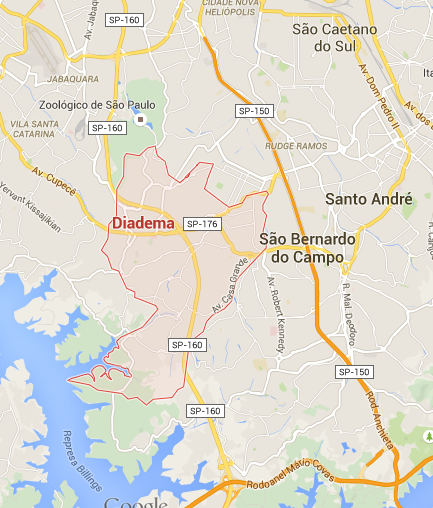
\includegraphics[scale=1.0]{diadema.png}
	\end{center}
	\ABNTEXchapterfont\small{fonte: Google Maps - 2015}
\end{mapa}
\par
Segundo o artigo, Diadema ocupou quase ininterruptamente, o primeiro lugar no número de homicídios da Grande São Paulo durante os anos 1980 a 2000. Em 1999, Diadema atingiu a taxa de 141 homicídios para cada 100 mil habitantes, uma das maiores do planeta.
\par
Depreende-se do artigo como Diadema chegou a essa situação:\\
1 - Explosão populacional;\\
2 - Total falta de infraestrutura;\\
3 - Loteamentos irregulares;\\
4 - Falta de saneamento e assistência médica;\\
5 - Descaso do poder público com a segurança;\\
6 - Corrupção policial (policiais indesejados eram enviados para lá)\\
\par
Fora isso, como consequência, frequentes eram os casos de enchentes, desabamentos, falta de energia, etc.,ou seja, o caos estava instalado na área. 
\par
A partir dos anos 90, sucessivos governos do Partido dos Trabalhadores começaram a tentar mudar esse cenário, oferecendo à população condições mais dignas de vida, com a construção de escolas, hospitais, implantação de saneamento básico e várias outras melhorias no bairro. Entretanto a criminalidade não diminuiu a níveis aceitáveis e uma pesquisa mais detalhada revelou uma grande movimentação imobiliária no município.
\par
Quando da verificação de quem eram os novos moradores, foi revelado que a cidade havia sido invadida pelo tráfico. Os traficantes da Grande São Paulo haviam escolhido Diadema para se fixar, graças às melhorias implementadas na cidade. O próximo passo sem dúvida foi mexer na polícia, que antes era subordinada a São Bernardo do Campo.
\par
A partir daí iniciou-se o processo de “Tolerância Zero' no município, que passou a ter seu próprio batalhão de polícia. Policiais corruptos foram desligados e presos após responderem processos disciplinares e a guerra contra o tráfico recomeçou de forma mais efetiva. Outra descoberta importante, no final de 2001, foi que o maior número de homicídios ocorria em bares, por volta das 23 horas. A polícia começou a usar a inteligência no lugar da repressão.
\par
Um projeto de lei foi enviado à Câmara Municipal propondo o fechamento dos bares as 23 horas. Foi realizado um grande debate entre donos de bares (que temiam a perda de receita e o desemprego de seus funcionários), vereadores e representantes da sociedade e o consenso foi que se o objetivo de reduzir a criminalidade fosse alcançado, o sacrifício seria feito. O projeto foi então aprovado por unanimidade. 
\par
Uma dissimulado “toque de recolher” foi implantado na cidade com essa medida e os resultados logo foram vistos com uma redução na taxa de homicídios para 8 por mês dentro ou nas proximidades dos bares, onde antes era de 30 a 40. O fechamento dos bares também afetou o tráfico de drogas que geralmente usa esses lugares como pontos de venda.
\par  
Quando do exemplo de New York, críticos demonstraram que outras cidades americanas tiveram decréscimo na criminalidade sem a implantação desse tipo de política. Vale a pena citar mais um trecho do trabalho do Instituto Braudel:
\begin{citacao}
	Nos bairros violentos do município de São Paulo	também houve quedas, \textbf{mas não tão grandes quanto em Diadema}
	Porém, as taxas de homicídio da Grande São Paulo (48) e Diadema (74) ainda são muito altas,
	especialmente se as comparamos com cidades como a Londres, Tóquio e Nova York, cujas taxas variam entre
	2 e 7 para cem mil. Nosso pesquisador de segurança pública, Cel. José Vicente da Silva, observa que “um
	índice de homicídios de 40 para cem mil ainda é indecente e não justifica comemorações antes de chegar
	a 20. Civilizado é chegar abaixo de 10”.\\
	Mas as recentes quedas de homicídios são fruto de um processo de civilização, ainda incompleto.
	Diadema representa bem esse processo. Representa a consolidação das comunidades na transição duma
	ocupação estilo “faroeste” para uma sociedade mais organizada. Este processo é complexo e envolve
	mudanças demográficas, novas formas de cooperação, 	ação mais efetiva dos governos municipal e estadual,
	aumentos no consumo popular, renovação da infraestrutura e das oportunidades culturais, incorporação
	de novas tecnologias, ampliação da atividade econômica com muitas improvisações modestas mas importantes e,
	sobretudo, o esforço de muitas famílias para conquistar	padrões de vida mais dignos.\cite[p. ~4, grifo do autor]{Braudel}
\end{citacao}
\par
Os moradores de Diadema aprenderam que “uma epidemia de homicídios é terrível, mas a tolerância aos homicídios é pior”\cite[p. ~5]{Braudel}.

\subsection{A tolerância zero em Natal - um estudo de caso}
\lettrine[lines=2, lhang=0.33, loversize=0.25]{O} Código de Trânsito Brasileiro (Lei 9.503  de 23 de setembro de 1997)  em seu Art. 306 estatui:
\begin{citacao}
	 Art. 276.  \textbf{Qualquer concentração de álcool} por litro de sangue ou por litro de ar alveolar sujeita o condutor às penalidades previstas no art. 165\\
	  Art. 165.  Dirigir sob a influência de álcool ou de qualquer outra substância psicoativa que determine dependência:       (Redação dada pela Lei nº 11.705, de 2008)\\
	  Infração - gravíssima;       (Redação dada pela Lei nº 11.705, de 2008) \\
	  Penalidade - multa (dez vezes) e suspensão do direito de dirigir por 12 (doze) meses.         (Redação dada pela Lei nº 12.760, de 2012)\\
	  Medida administrativa - recolhimento do documento de habilitação e retenção do veículo, observado o disposto no § 4o do art. 270 da Lei no 9.503, de 23 de setembro de 1997 - do Código de Trânsito Brasileiro.      (Redação dada pela Lei nº 12.760, de 2012)\\
	  Parágrafo único. Aplica-se em dobro a multa prevista no caput em caso de reincidência no período de até 12 (doze) meses. (Redação dada pela Lei nº 12.760, de 2012) \cite{CTB}
\end{citacao}
\par
Por ser uma cidade turística, de clima quente, uma vida noturna agitada, Natal infelizmente possui um número expressivo de acidentes causado por pessoas que dirigem após  o consumo de bebidas alcoólicas.
\par
Há aproximadamente dois anos, o capitão da Polícia Militar Ean Styvenson Valentin (na época tenente) desencadeou uma verdadeira operação de guerra
contra motoristas embriagados no município. Comandos foram realizados altas horas da noite em busca desse tipo de condutores e o resultado não
poderia ter sido outro: um grande número de prisões e apreensões de veículos. A reação logo veio, com ameaças de morte ao então tenente,
deboches nas redes sociais no sentindo de desmoralizá-lo e, no perceber do autor, tentativas administrativas para fazê-lo parar\footnote{N.A. Veja em  \href{http://tribunadonorte.com.br/noticia/apa-s-anaoncio-de-saa-da-styvenson-retorna-a-coordenaa-a-o-da-lei-seca/310527?utm_campaign=noticias&utm_source=20150408}{Cap. Styvenson} - acesso em 2.9.2015} (corte de verbas, transferência).
\par
No entanto o bom senso prevaleceu, o capitão perseverou na sua atuação e, segundo reportagem disponível no site G1 \footnote{N.A. Disponível em:\href{http://g1.globo.com/rn/rio-grande-do-norte/noticia/2015/06/cai-14-numero-de-natalenses-que-admitem-beber-e-dirigir-diz-ministerio.html}{Queda nos índices} - acesso em 29.6.2015} (globo.com) caiu em 14 \% o número de motoristas que admitem dirigir após beber. Em paralelo, outras apreensões são feitas, como armas, drogas e mesmo foragidos da polícia.
\par
No fechamento do presente trabalho o autor conseguiu uma longa e proveitosa conversa com o Capitão Styvenson Valentim. Os detalhes principais são mostrados no apêndice B. Como conclusão preliminar pode-se constatar que o Capitão possui os requisitos e características fundamentais para compor uma eventual equipe implementadora da política aqui proposta.
\hypertarget{Sty1}{} 
\par
As acusações continuam no sentido de desmoralizar o rigor da fiscalização e parar esse tipo de ação, como a insinuação de excessos por parte dos policiais nas
operações, demora na liberação dos presos, exigências de contraprova, etc., enfim, embora com grande aceitação por parte da população, existem ainda pessoas inconformadas com a política de “tolerância zero” do binômio álcool-direção.Veja o \hyperlink{B5}{subitem B5} da entrevista com o Cap. Styvenson.
\hypertarget{Sty}{}
\par
A cidade de Mossoró, localizada na região oeste do RN e segunda maior aglomeração urbana,  também começou a ser fiscalizada no primeiro semestre de 2015 e novamente a historia  ocorrida em Natal se
repete, com pessoas “incomodadas” pela perda de liberdade. Mas com o tempo, a própria população irá começar a fiscalizar isso também.
Vale ressaltar aqui dois casos semelhantes: o primeiro foi a proibição de fumar em locais fechados de acesso público e o segundo o uso obrigatório do cinto de segurança. Nesses dois casos, hoje a própria população fiscaliza essas ações e até chamam a polícia em caso
de desrespeito. Sobre isso veja o \hyperlink{B13}{subitem B13} da entrevista.
\hypertarget{Nat}{}
\par
De forma a adiantar o também descrito no Apêndice B, alguns números impressionantes da sua atuação: desde o início da operação lei seca (aproximadamente 2 anos) foram feitas 50.000 abordagens, 7.000 Carteiras de Habilitação apreendidas e 1.200 prisões por embriagues ao volante. Sem dúvida uma política de tolerância zero. Veja a \hyperlink{B10}{subitem B10} da entrevista. 
\par
O trecho mais marcante do depoimento do Cap. Styvenson, e um justificador da necessidade da implantação da Política de Tolerância Zero, vale ser aqui destacado:
\begin{citacao}
	Isso eu presenciei. O pai, está indo para a delegacia com o dinheiro na mão, contando de cabeça baixa para ver se tem dinheiro para pagar a fiança, eu ouço um grito de dentro da jaula: “paga essa p* aí véio, pra gente ir tomar outra”. Na minha cabeça veio, logo no momento,  o pai passou a vida toda bebendo com o filho, não tem respeito nenhum, perdeu, acabou.
\end{citacao}
\par
Como já dito anteriormente, esse tipo de procedimento deve ser usado quando a situação exige e cada caso deve ser analisado individualmente. Agora resta a pergunta: e para os casos mais graves e que transcendem as fronteiras do estado, tal como o tráfico de entorpecentes, contrabando, roubos a bancos, etc.,
será que é possível implantar uma política de tolerância zero para isso também aqui em Natal?
\par
Para subsidiar o presente estudo, deve-se inicialmente entender como a população natalense percebe toda a legislação que a cerca. Isso será abordado no próximo capítulo.

% ----------------------------------------------------------
\chapter{O Índice de Percepção ao Cumprimento das Leis - IPCL}

\section{Definições e Metodologia de Cálculo}
\lettrine[lines=2, lhang=0.33, loversize=0.25]{O} {Índice} de Percepção ao Cumprimento das Leis - Brasil é um trabalho de pesquisa publicado semestralmente pela Faculdade de Direito da Fundação Getúlio Vargas de São Paulo  e tem por objetivo:
\begin{citacao}
	O objetivo do \textit{Índice de Percepção as Leis no Brasil (IPCL-Brasil)} é medir, de forma sistemática, a percepção dos brasileiros em relação ao respeito às	leis e às determinações de algumas autoridades que estão diretamente envolvidas	com o cumprimento das leis.\\
	\ldots\\
	De modo geral, o \textit{Índice de Percepção as Leis no Brasil (IPCL-Brasil)} retrata a relação do indivíduo com o Estado de direito, observando o respeito daquele às leis, bem como às autoridades que devem fazer com que as leis sejam cumpridas.\cite[p. ~2-3]{FGV}
\end{citacao}

\section{Elaboração do questionário e Definição da amostra}
\lettrine[lines=2, lhang=0.33, loversize=0.25]{P}{ara} o cálculo do IPCL-Natal, foi replicado e adaptado o mesmo questionário utilizado pela FGV para o IPCL-Brasil, com duas alterações: Foi retirada
a definição cor/raça do questionário, visto entender-se que é um parâmetro subjetivo (segundo o IBGE, quem define sua cor/raça é o 
próprio cidadão) e na questão de confiança nas instituições públicas foi adicionada a opção “nenhuma delas”, pois esse é um indicativo
de aparente descaso com as instituições oficiais.  O questionário e as respostas obtidas encontram-se no Apêndice A do presente trabalho.
\par
O método de aplicação do questionário foi bem aleatório, inicialmente se utilizou a rede pessoal do autor que repassavam a seus pais, amigos, namoradas;
depois ficou disponível na internet para quem quisesse preencher por três meses aproximadamente; pessoas foram selecionadas ao acaso pelo autor:
o entregador de água, o vendedor de frangos, o jornaleiro, enfim, pessoas do convívio no dia a dia.
\par
Após o período de aplicação, foram contabilizados 193 questionários respondidos e devidamente embaralhados. Atualmente, não existe a menor
possibilidade de identificação de quem respondeu determinado questionário. A internet foi uma grande aliada, visto prover o tão desejável
anonimato.
\par
Com 193 questionários respondidos, obtém-se um grau de confiança de 95\% e erro amostral de aproximadamente 7\% para a população de Natal \footnote{N.A. SANTOS, Glauber Eduardo de Oliveira. Cálculo amostral: calculadora on-line. Disponível em:\href{http://www.calculoamostral.vai.la}{Calculadora amostral} Acesso em: 29.6.2015.}.
\par
Quanto aos percentuais amostrais, ou seja, nas faixas de idade definidas para a população, infelizmente obteve-se um BIAS (o VIÉS estatístico) um pouco tendencioso para o segmento mais jovem da população. A explicação pode ser dada através de dois motivos: como a pesquisa foi deflagrada de um ambiente universitário, era de se esperar uma maior participação de pessoas nessa faixa de idade; o outro foi a verificada resistência a responder perguntas quanto maior a idade do entrevistado. Talvez em uma próxima pesquisa (se houver), seja inserida uma variável de controle para isso.
\par
A tabela 1 reflete o acima dito:

\begin{table}[!htpb]
	\begin{center}
		\caption{Cálculo dos percentuais amostrais}%
		\label{Tabela 1}
		\begin{tabular}{cccccc}
			\hline\\
			Idade & Homens & Mulheres & Total & Previsto \% & Obtido \% \\\\
			\hline
			\hline\\
			15 a 34 anos & 144744 & 154561 & 299305 & 47 & 64 \\
			35 a 59 anos & 118098 & 134518 & 253616 & 40 & 29\\
			mais 60 anos & 33111  & 50828  & 83939  & 13 & 7 \\\\
			\hline
		\end{tabular}%
	\end{center}
	\ABNTEXchapterfont\small{Fonte:Produzida pelo autor - agosto de 2015 - Censo IBGE 2010}
\end{table}
\FloatBarrier
\par
\subsection{Definição dos Subíndices e Indicadores}

Segundo o relatório, para a construção do IPCL-Brasil, 2 subíndices são criados: o de percepção e o de comportamento :

\begin{citacao}
O \textbf{subíndice de percepção} é construído a partir de 4 indicadores quais sejam: (i) \textit{indicador de \textbf{instrumentalidade}}, que
mede a percepção das perdas associadas ao descumprimento da lei -- sanções; (ii) \textit{indicador de \textbf{moralidade}}, que mede a
percepção dos entrevistados sobre o quanto é certo ou errado realizar determinada conduta que esteja em desconformidade com a lei; (iii)
\textit{indicador de \textbf{controle social}}, que mede a percepção de reprovação social a determinados tipos de comportamento de
descumprimento da lei; e (iv) \textit{indicador de \textbf{legitimidade}}, que mede a percepção sobre a obediência à lei e às ordens de
autoridades que devem fazer com que a lei seja cumprida.

Para o \textit{indicador de \textbf{instrumentalidade}} perguntamos aos entrevistados qual a probabilidade de serem punidos por comportamentos
de desrespeito à lei. Esses comportamentos foram construídos a partir de casos do cotidiano, pelos quais a maioria dos entrevistados pode
passar. As possibilidades de resposta foram: muito provável, um pouco provável, um pouco improvável ou muito improvável.

Para o \textit{indicador de \textbf{moralidade}}, pedimos aos entrevistados que considerassem seus próprios sentimentos sobre o que é certo e
errado, e respondessem o quão certo ou errado acham que são os comportamentos citados. As respostas possíveis foram: muito errado, um pouco
errado, quase nada errado ou nada errado.

Para o \textit{indicador de \textbf{controle social}}, solicitamos aos entrevistados que pensassem em seus amigos e em pessoas adultas próximas
a eles, as quais conhecem bem. A partir daí, perguntamos se na hipótese de serem vistos fazendo algumas das situações citadas, o quanto os
seus amigos desaprovariam a sua conduta, sendo as possibilidades de resposta: desaprovariam muito, desaprovariam um pouco, quase nada ou nada.

Por fim, para o \textit{indicador de \textbf{legitimidade}}, pediu-se aos entrevistados que considerassem oito afirmações sobre o
comportamento das pessoas diante da lei e das ordens de algumas autoridades e dissessem o quanto concordavam com cada uma das afirmações,
sendo as respostas possíveis: concorda muito, concorda um pouco, discorda um pouco ou discorda muito.

O \textit{subíndice de \textbf{comportamento}}, por sua vez, é construído a partir do indicador de conformidade com a lei que retrata a
frequência com que os entrevistados declaram ter realizado condutas que representam desobediência à lei. Esse indicador é elaborado com base
em dez situações diferentes. Perguntamos aos entrevistados com que frequência realizaram cada uma dessas condutas nos últimos 12 meses, sendo
as possibilidades de resposta: frequentemente, algumas vezes,poucas vezes, quase nunca ou nunca.

A existência dos dois subíndices, o de \textbf{comportamento} e o de \textbf{percepção} permite  que, de alguma forma, controlemos as
respostas dos entrevistados minimizando a sobrevalorização das respostas referentes ao próprio comportamento. A necessidade de um controle das
respostas se deve ao fato de que os entrevistados, ao se referirem ao próprio comportamento, tendem a responder que são mais “aderentes” ao
comando legal do que quando avaliam o mesmo comportamento realizado por outras pessoas.\cite[p. ~3-4]{FGV}
\end{citacao}
Resumindo: 
\begin{itemize}
	\item subíndice de percepção = (indicador de instrumentabilidade + indicador de moralidade + indicador de controle social + indicador de legitimidade)/4
	\item subíndice de comportamento = indicador das questões (7 + 11 + 15 +19 + 23 + 27 + 31 + 35 + 39 + 43)/10
\end{itemize}

\subsection{Metodologia de Cáculo do IPCL}
O IPCL-Natal é calculado da mesma forma que o IPCL-Brasil:
\begin{citacao}
	As perguntas que formam o questionário do IPCLBrasil têm quatro respostas. Identifica-se cada resposta atribuindo-se a ela um indexador n, que também corresponderá a um valor atribuído àquela resposta. Assim sendo, à primeira resposta, ou seja, à resposta 0, atribui-se o valor 0. À última resposta atribui-se o valor máx,que será 3. Consequentemente n = 0, 1, 2, 3. Por exemplo, às respostas (i) discordo muito; (ii) discordo um pouco; (iii) concordo um pouco; (iv) concordo muito, atribuem-se respectivamente, os valores 0, 1, 2 e 3. Essa metodologia de atribuição de valores cardinais tem a vantagem de ser simples e direta para aferir a resposta numérica das pessoas. Tem a desvantagem de, implicitamente, assumir que a diferença entre as respostas é igual, o que pode não ser verdade, já que se trata de respostas ordinais.\\
	A resposta n da questão q é chamada de nq . O valor que se atribui a nq é n,	ficando claro que valor(nq ) = n. Por exemplo, a resposta 0 (ou primeira resposta) da questão q = 2 é 0, ou seja, valor(02) = 0.
	Em seguida, os valores são ponderados de acordo com a proporção de pessoas	que escolheram aquela resposta. A proporção de pessoas que escolheram a resposta n da questão q é indexada pela variável . Com isso, obtém-se o primeiro valor	intermediário refletindo a nota média de cada questão, escalonada entre 0 e máx,cuja fórmula é a seguinte:\\
	{\fontsize{12}{12}\fontfamily{phv}\selectfont
	$media_{q}=\sum\limits_{n_{q}=0}^{max} n_{q}w_{q}$}
	
	em que, $media_{q}$ é a nota média obtida na questão q.\\
	Note que a média da questão tem um valor mínimo de 0, quando $w_{q}=1$ e um valor máximo igual a \textit{max} quando $w_{maxq} = 1$.\\	
	Normalizamos a média para ir de 0 a 10, razão pela qual dividimo-la pela pontuação máxima e multiplicamos a média de cada questão por 10. Ou seja, calcula-se a nota normalizada da questão \textit{q}, $nn_{q}$ , da seguinte forma:\\
	{\fontsize{12}{12}\fontfamily{phv}\selectfont
	$nn_{q} = \frac{media_{q}}{max_{q}} x 10$}.\\
	Dado que a $media_{q}$ fica entre 0 e $max_{q}$ então é fácil concluir que $nn_{q}$ fica entre 0 e 10.
	Em seguida, para cada bloco de questões, calculam-se subíndices de percepção, de acordo com o número de questões respondidas em cada bloco, sendo que cada uma das questões tem o mesmo peso. O subíndice de percepção do bloco, IPCLb , é dado considerando as questões restritas àquele dado bloco,{\fontsize{12}{12}\fontfamily{phv}\selectfont $nn_{q}:IPCL_{b}=\sum_{qcb}^{} nn_{q}/8$}
	Semelhantemente se faz para os demais 5 blocos.\\
	A seguir se calcula o IPCL de percepção agregando os indicadores de instrumentalidade, moralidade, controle social e legitimidade, da seguinte forma:\\
	{\fontsize{12}{12}\fontfamily{phv}\selectfont
	$IPCL_{p}=\sum\limits_{b=1}^{4} \frac{IPCL_{b}}{4}$}\\
	Finalmente, o IPCLBrasil é obtido pela média ponderada de ambos os subíndices, sendo 80\% para o subíndice de percepção e 20\% para o subíndice de comportamento. Cada questão tem o mesmo peso individual dentro do subíndice.\\
	Portanto, o IPCLBrasil é dado por:\\
	{\fontsize{12}{12}\fontfamily{phv}\selectfont
		$IPCL_{Brasil}= 0,2 x IPCL_{c} + 0,8 x IPCL_{p}$}\\
	\cite[p. ~7-8]{FGV}
\end{citacao}
\par
Sem adentrar nos cálculos matemáticos, os quais podem facilmente ser reproduzidos mediante o uso de qualquer planilha eletrônica (no presente caso foi utilizado o LibreOffice Calc), o IPCL-Natal calculado
foi de \textbf{IPCL-Natal= 4,42} conforme demonstrado sucintamente na tabela 2.

\begin{table}[!htpb]
	\begin{center}
		\caption{Cálculo do IPCL-Natal - 2015}%
		\label{Tabela 2}
		\begin{tabular}{llc}
			\hline\\
			Subíndices &  Indicadores & Valor obtido \\\\
			\hline
			\hline
			Comportamento & &5,74 \\
			\hline\\
			&Instrumentabilidade& 3,52\\
			&Moralidade& 5,74\\
			&Controle social& 3,59\\
			&Legitimidade& 3,52\\\\
			\hline
			Percepção& &4,09\\		 		 		 
			\hline\\
			\textbf{IPCL-Natal}& &\textbf{4,42}\\\\
			\hline
		\end{tabular}%
	\end{center}
	\ABNTEXchapterfont\small{Fonte: Produzida pelo autor - agosto de 2015}%
\end{table}
\FloatBarrier
\par
Nota-se que os indicadores com menor nota foram Instrumentabilidade, ou seja, existe a percepção que a probabilidade de punição por desvios de conduta é baixa e o de Legitimidade que sugere uma desídia de comportamento diante das leis e das autoridades. Pelo outro lado o indicador de Moralidade mostra que as pessoas tem a consciência do certo e errado, embora não necessariamente isso seja um empecilho para frear um desvio da lei. Deve ser destacada a seguinte observação feita pelos autores do IPCL-Brasil:
\begin{citacao}
	É importante destacar que o IPCLBrasil de 7,0 pontos não representa um
	grau superior a 50\% de respeito da população às leis, mas, sim, que a \textbf{percepção
		do cidadão brasileiro} em relação ao cumprimento das leis chegou a 7,0 pontos
	em uma escala de 0 a 10, sendo 10 um total comprometimento com o cumprimento das leis.\cite[p ~10, grifo do autor]{FGV}
\end{citacao}
\par
Não é do escopo do presente trabalho esmiuçar o IPCL-Natal, mas sim utilizá-lo como subsidio para a análise SWOT adiante, bem como a retirada
de elementos de interesse para a política de tolerância zero, através do processamento dos dados coletados.

\section{Caracterização da área de estudo: O Município de Natal}

\lettrine[lines=2, lhang=0.33, loversize=0.25]{N}{atal} é a capital do estado do Rio Grande Norte, região nordeste do Brasil. É o município central da Região Metropolitana de Natal e:
\begin{citacao}
A RMN está localizada na microrregião do litoral oriental do RN \ldots  que compreendia em 2012 dez municípios: Natal, Parnamirim, Nísia Floresta,São Gonçalo do Amarante, Macaíba, Ceará Mirim, Extremoz, São José de Mipibú, Monte Alegre e Vera Cruz.\\
\ldots\\
Todos os 10 municípios que compõem a Região Metropolitana de Natal, estão territorialmente muito próximos a Natal, favorecendo assim a grande mobilidade  entre esses municípios e, também, deles em relação a Natal, dado a distância não ultrapassar 35 km.\\
\ldots\\
No que diz respeito à metropolização, este é definido por ser Natal, cidade polo e responsável pelos processos de conurbação e de transbordamento populacional com os municípios de Parnamirim e São Gonçalo do Amarante, de forma mais expressiva  nas últimas décadas. Esses dois municípios são os mais dinâmicos  da região e vem passando por processos de urbanização e incremento populacional  mais significativo do que os demais municípios, os quais mantêm uma relação  de dependência muito maior com a cidade polo, sendo menos desenvolvidos, com grau de urbanização inferior e apresentando ainda fortes características rurais. \cite[p. ~29-31]{Pessoa}
\end{citacao}

De acordo com o censo de 2010 do IBGE, o município de Natal possui as seguintes características principais(Tabela 3):

\begin{table}[h]
	\begin{center}
	\caption{Características do Município de Natal - 2010}%
	\label{Tabela 3}
	\begin{tabular}{llc}
		\hline		
		População & &803.739 ha. \\
		&do sexo masculino & 377.947 ha. \\
		&do sexo feminino & 425.792 ha. \\
		\hline
		alfabetizados & &84 \%\\
		IDHM & &0,763 \\
		Índice de GINI & &0,61 \\
		\hline
	\end{tabular}
	\end{center}
	\ABNTEXchapterfont\small{Fonte: Produzida pelo autor - agosto de 2015 - IBGE\cite{IBGE} - IPEA-PNUD\cite{IPEA}}%
\end{table}
\FloatBarrier
\par
O Índice de Desenvolvimento Humano (IDHM) - Natal é 0,763, em 2010, o que situa esse município na faixa de Desenvolvimento Humano Alto (IDHM entre 0,700 e 0,799). A dimensão que mais contribui para o IDHM do município é Longevidade, com índice de 0,835, seguida de Renda, com índice de 0,768, e de Educação, com índice de 0,694. 
\begin{mapa}[!htb]
	\caption{\label{Mapa2}Município de Natal - RN}
	\begin{center}
		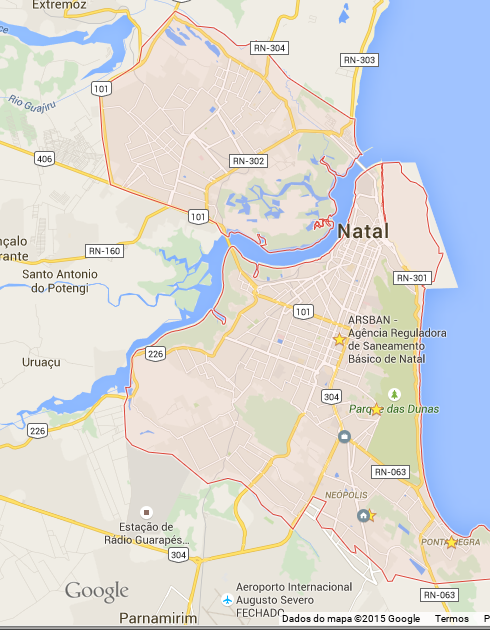
\includegraphics[scale=0.9]{natal.png}
	\end{center}
	\ABNTEXchapterfont\small{fonte: Google Maps - 2015}
\end{mapa}
\FloatBarrier
\par

\par
O índice de Gini é um instrumento usado para medir o grau de concentração de renda. Ele aponta a diferença entre os rendimentos dos mais pobres e dos	mais ricos. Numericamente, varia de 0 a 1, sendo que 0 representa a situação de total igualdade, ou seja,	todos têm a mesma renda, e o valor 1 significa completa desigualdade de renda, ou seja, se uma só pessoa detém toda a renda do lugar.
\par
Possui portanto um alto nível de desigualdade social, que pode ser visualizado
na foto da região composta pelas ruas da ladeira do sol e rua do motor (IDHM acima de 0,9 a esquerda e ao redor de 0,45 a direita) e comparável a famosa foto da favela Paraisópolis em São Paulo.(Fotos 3 e 4)
\begin{foto}[!htpb]
	\centering
	\begin{minipage}{.47\linewidth}
		\caption{\label{Foto1}Ladeira do Sol em Natal}	
		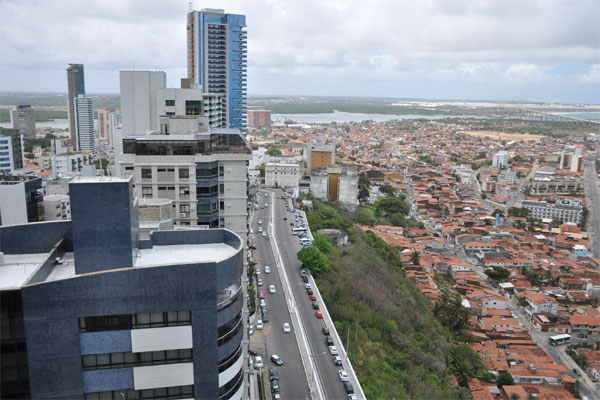
\includegraphics[width=\linewidth]{Natal_paraisopolis.jpg}
		\ABNTEXchapterfont\small{fonte:Jornal Tribuna do Norte - 01/12/2014}
	\end{minipage}
	\hspace{.05\linewidth}
	\begin{minipage}{.46\linewidth}
		\caption{\label{Foto2}Favela Paraisópolis - SP}
		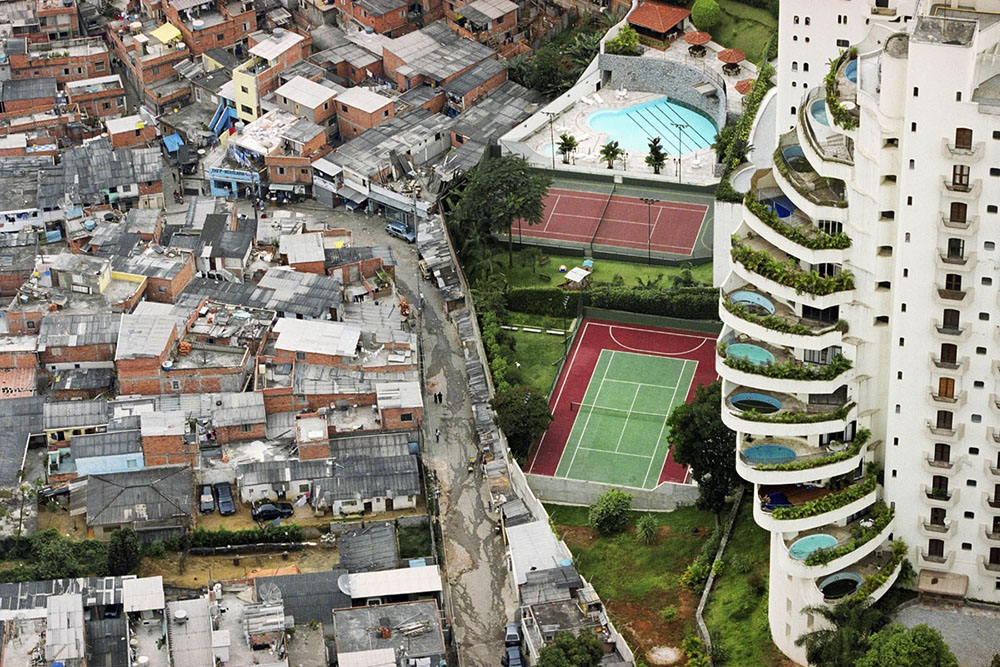
\includegraphics[width=\linewidth]{Paraisopolis.jpg}
		\ABNTEXchapterfont\small{fonte:\href{http://www.tucavieira.com.br/A-foto-da-favela-de-Paraisopolis}{Favela Paraisópolis}}
	\end{minipage}
\end{foto}
\par
Outro índice preocupante o crescente aumento da taxa de homicídios no município, como mostra o Gráfico 3. A taxa de homicídios em 2013 foi de absurdos 62,30/100.000 ha. óbitos para 26,99/100.000 ha. a nível nacional. Coincidência ou não e independente de qualquer crítica no sentido político, o município viveu uma situação de abandono exatamente a partir de 2008 (o paradigma de Zimbardo novamente!) quando a prefeita ao longo de quatro anos de mandato não conseguiu montar um governo de coalizão e assim tornou sua administração ingovernável. Exatamente nessa época o índice de criminalidade rompeu a média nacional (gráfico 3). Para coroar a situação, o mesmo ocorreu com a governadora eleita em 2010, dessa vez deixando todo o Estado do Rio Grande do Norte em situação de abandono. O autor buscou junto aos órgãos de segurança pública dados de 2014 e 2015 para verificar um eventual declínio nas tendências mas não logrou sucesso.

\par
Em meticuloso trabalho de pesquisa sobre a mortalidade violenta na Região Metropolitana de Natal até o ano de 2007 (o índice de homicídios foi de 28,32/100.000 ha. nesse ano), o Observatório das Metrópoles de Natal concluiu que:
\begin{citacao}
	A análise dos dados do Sistema de Informações de Mortalidade (SIM) do Datasus para Região Metropolitana de Natal evidencia que
	as taxas de homicídio apresentou uma tendência de crescimento evidente, sobretudo, a partir de 2004.No período analisado, entre
	1998 e 2007, a taxa de homicídio na RMN praticamente dobrou.\\
	A mortalidade por criminalidade violenta é um fenômeno de homens jovens. Os resultados ora apresentados ratificam essa tese e
	chamam a atenção para o fato de que está aumentando o risco de	homicídio entre adolescentes, grupo etário entre 15 e 19 anos, nos
	municípios da região metropolitana analisada.\cite[p. ~92]{Bezerra}
\end{citacao}\begin{grafico}[!htb]
\begin{center}
	\caption{Homicídios para 100.000 habitantes}
	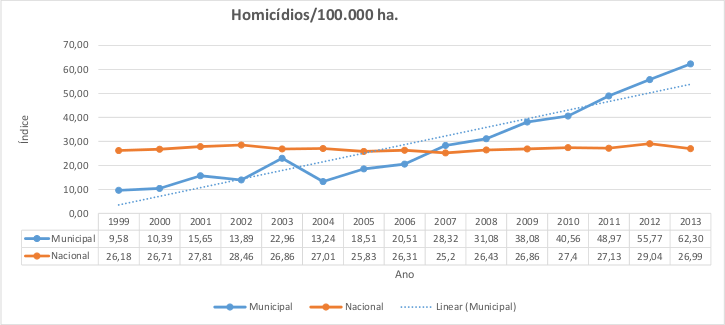
\includegraphics[scale=0.75]{Homicidios-geral.png}
\end{center}
\ABNTEXchapterfont\small{fonte: Produzido pelo autor - agosto de 2015 - DATASUS}
\label{Homicidios}
\end{grafico}
\FloatBarrier
Conseguiu-se em 6 anos novamente mais que dobrar o índice!!! Entretanto se o índice do gráfico 3 é absurdo, o que dizer dos gráficos 4 e 5 que mostram nas faixas de idade de 15 a 19 anos e 20 a 29 anos?
\begin{grafico}[h]
	\begin{center}
		\caption{Homicídios para 15-19 anos/100.000 habitantes}
		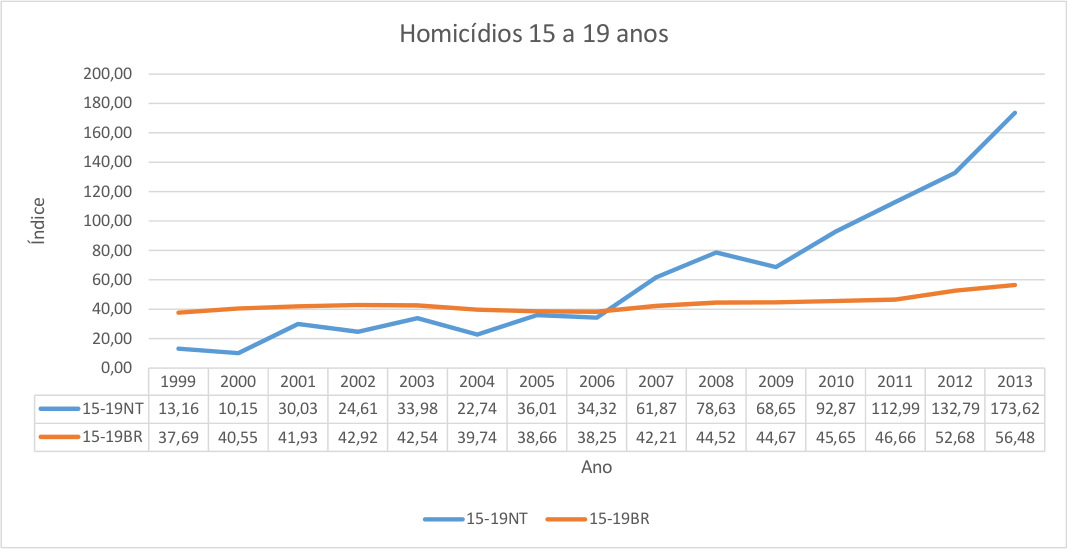
\includegraphics[scale=0.5]{juventude-15-19.png}
	\end{center}
	\ABNTEXchapterfont\small{fonte: Produzido pelo autor - agosto de 2015 - DATASUS}
	\label{Homicidios15-19}
\end{grafico}
\FloatBarrier
\par
Para o ano de 2013, o índice de homicídios de jovens na faixa entre 15 e 19 anos foi de 173,63/100.000 ha. para Natal enquanto o índice nacional foi de 56,48/100.000 ha. ou seja, quase três vezes maior (gráfico 4).
\begin{grafico}[h]
	\begin{center}
		\caption{Homicídios para 20-29 anos/100.000 habitantes}
		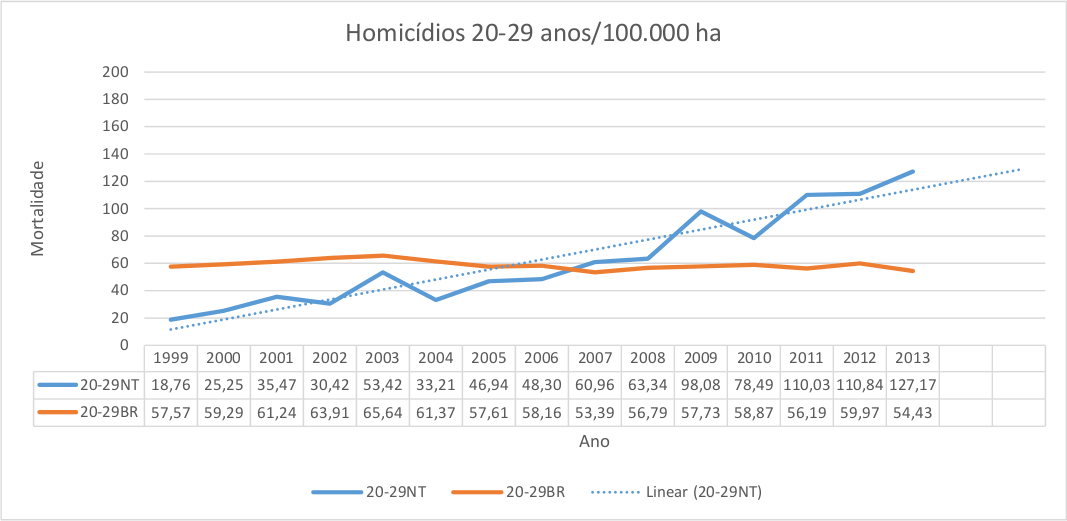
\includegraphics[scale=0.5]{juventude-20-29.png}
	\end{center}
	\ABNTEXchapterfont\small{fonte: Produzido pelo autor - agosto de 2015 - DATASUS}
	\label{Homicidios20-29}
\end{grafico}
\FloatBarrier
\par
E para a faixa 20 a 29 anos no mesmo ano de 2013 foi 127,17/100.000 ha. para Natal contra 54,43/100.000 ha. para o país, um pouco mais que o dobro (gráfico 5).
\par
Algumas perguntas devem ser feitas:\\
-- Essa alta taxa de homicídios na população jovem é decorrente da maior exposição nessa faixa de idade ou é resultante da vulnerabilidade a que ela está sujeita? Um disciplinamento maior teria surtido algum resultado?\\
-- O que aconteceu com Natal em 2003 para ocorrer um pico de homicídios? \\
-- Por que, a partir de 2007, foi rompida a barreira nacional e o crescimento dos homicídios ficou tão acentuado? (Uma hipótese já foi levantada)
\par
Infelizmente o autor não possui as respostas.


\section{Resultados}
\lettrine[lines=2, lhang=0.33, loversize=0.25]{D}{a} análise da pesquisa pode-se extrair alguns gráficos de maior interesse para esse trabalho (existem inúmeras possibilidades). 
\par
Sem dúvida, o item mais impactante é a confiança da população nas instituições, como mostra o gráfico 6. Apesar da grande maioria ter dito não confiar em nenhuma instituição, verifica-se que o Ministério Público, as Forças Armadas e a Igreja ainda possuem uma certa credibilidade. A Polícia encontra-se desacreditada e os Partidos Políticos conseguiram ficar como últimos colocados (sem dúvida indicadores muito perigosos).
\par
Essas colocações serão discutidas na análise SWOT mais a frente.
\par
\begin{grafico}[!htpb]
	\begin{center}
	\caption{Confiança nas instituições - 2015}
	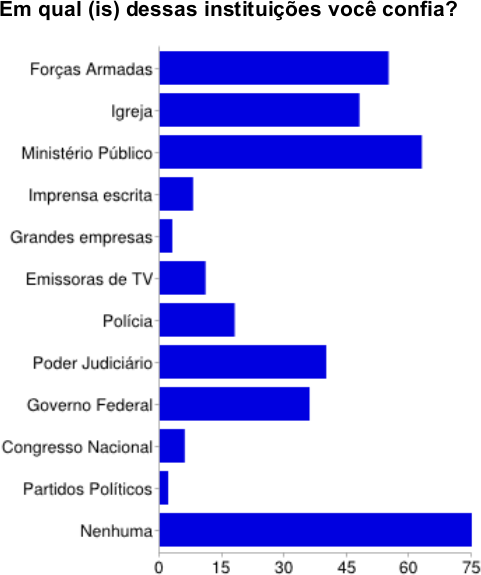
\includegraphics[scale=0.4]{confianca.png}
	\end{center}
	\ABNTEXchapterfont\small{Fonte: elaborado pelo autor - agosto de 2015}
	\label{Confiança}
\end{grafico}

\begin{grafico}[!htpb]
	\caption{Dificuldade de implantação de uma política de tolerância zero em Natal}
	\begin{center}
	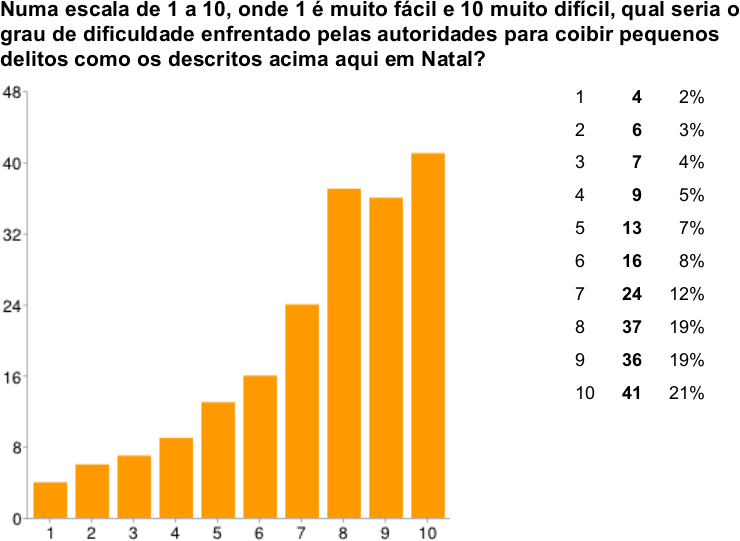
\includegraphics[scale=0.5]{percepcao.png}
	\end{center}
	\ABNTEXchapterfont\small{Fonte: elaborado pelo autor agosto de 2015}
	\label{Percepcao}
\end{grafico}
\par
Outro dado importante é a percepção da população quanto a dificuldade da implantação de uma política de tolerância zero no município. Verifica-se que 71\% dos entrevistados classificaram com nota maior ou igual a 7 (maior dificuldade) O sentimento presente para o autor é que a população tem consciência de sua baixa percepção ao cumprimento das leis e que isso reflete na nota dada. O gráfico 7 mostra o comentado.

\section{Índice de conformidade}
O gráfico 8 mostra de maneira geral a porcentagem dos entrevistados que cometeram alguma transgressão das perguntas formadoras do Subíndice de Conformidade com as leis. O universo analisado para esse gráfico foram as 193 respostas, e contadas somente os casos em que a resposta foi ter feito pelo menos uma vez nos últimos 12 meses. 
\par
\begin{grafico}[!htpb]
	\caption{Indicador de Conformidade - Geral - NATAL, 2015}
	\begin{center}
		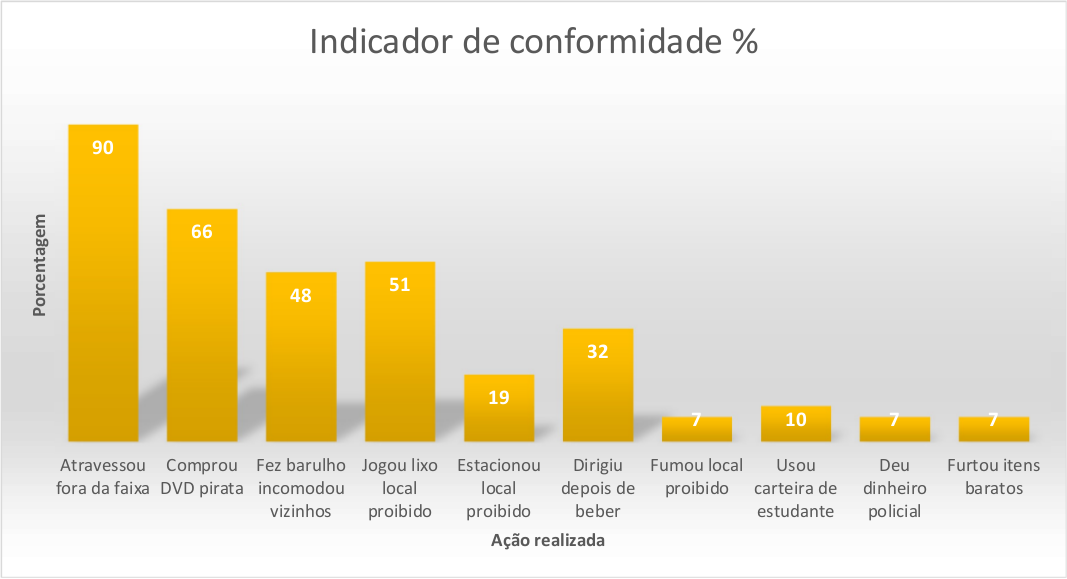
\includegraphics[scale=0.55]{Conformidade_geral.png}
	\end{center}
	\ABNTEXchapterfont\small{Fonte: elaborado pelo autor - agosto de 2015}
	\label{Conf_geral}
\end{grafico}
\FloatBarrier
\hypertarget{Conf1}{}
\par
Para os gráficos estratificados do Indicador de Conformidade (9 a 12) foram desconsideradas as respostas “Nunca”, as demais reunidas em um único grupo e estratificadas por sexo, faixa etária, escolaridade e renda. Para isso, partiu-se do princípio que uma política de tolerância zero não permite um único desvio, tanto faz ter feito uma ou várias vezes. As porcentagens referem-se somente ao universo dos que admitiram ter feito a transgressão. 
\par
Nota-se que esse número é relativamente alto em alguns casos o que sugere um possível caso de desobediência civil, como será mostrado \hyperlink{T1}{na Análise SWOT}.
\hypertarget{beb2}{}
\begin{grafico}[!htpb]
	\caption{Indicador de Conformidade - Sexo - NATAL, 2015}
	\begin{center}
		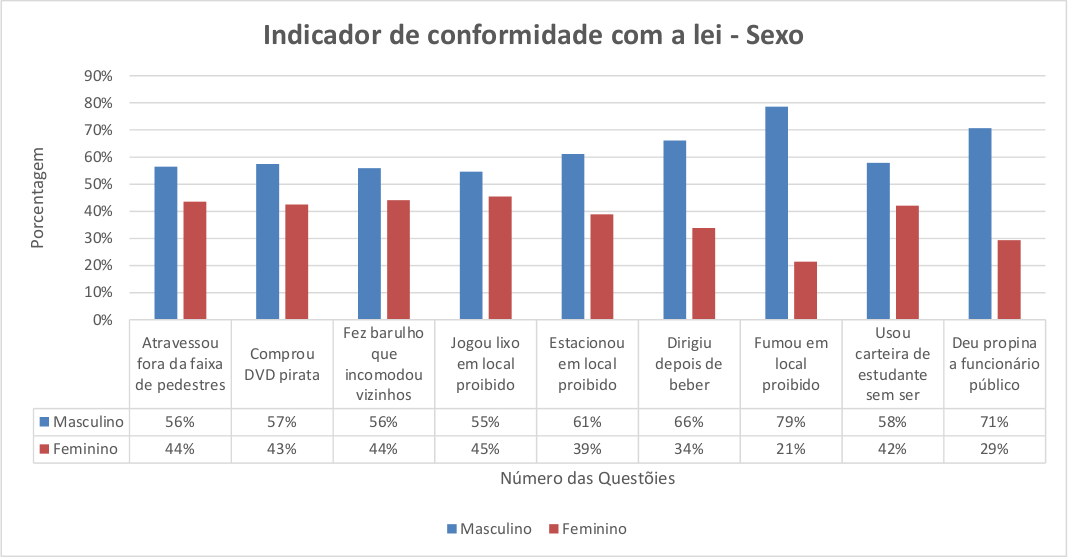
\includegraphics[scale=0.5]{Conformidade-sexo.png}
	\end{center}
	\ABNTEXchapterfont\small{Fonte: elaborado pelo autor - agosto de 2015}
	\label{Conf_sexo}
\end{grafico}
\FloatBarrier
\par
Nota-se no gráfico 9 a predominância do sexo masculino nas transgressões. Tendo em vista a ação da operação Lei Seca em Natal uma especial atenção deve ser dada ao item “Dirigiu depois de beber”, com 66\% dos entrevistados que admitiram ter feito isso ser do sexo masculino. Sbre isso, veja a interessante colocação do Cap. Styvenson em sua entrevista \hyperlink{B2}{subitem B2}.
\begin{grafico}[!htpb]
	\caption{Indicador de Conformidade - Faixa de Idade - NATAL, 2015}
	\begin{center}
		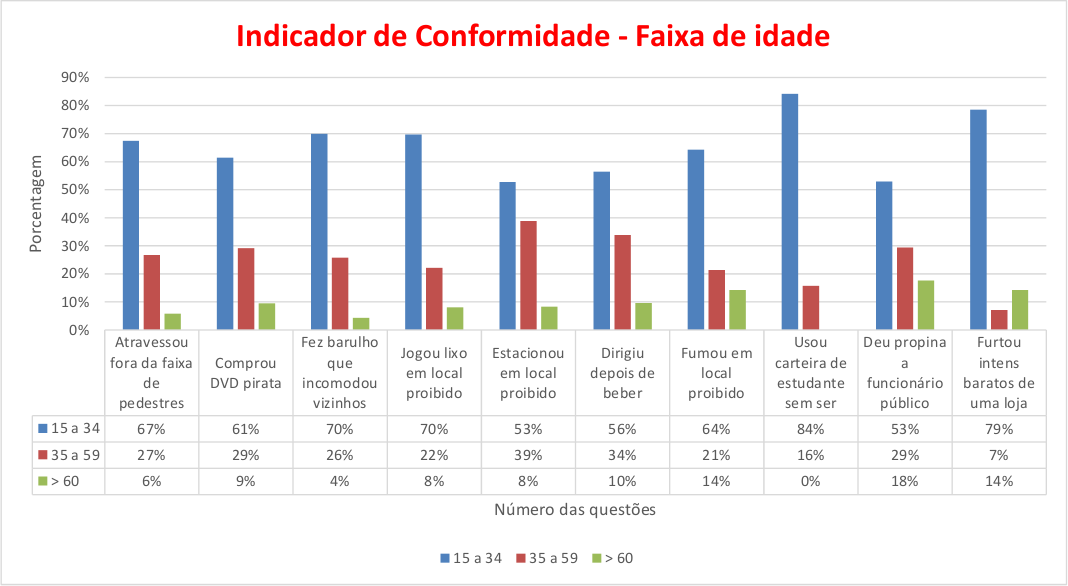
\includegraphics[scale=0.5]{Conformidade-idade.png}
	\end{center}
	\ABNTEXchapterfont\small{Fonte: elaborado pelo autor - agosto de 2015}
	\label{Conf_idade}
\end{grafico}
\FloatBarrier
\par
Não é de se estranhar que os mais jovens sejam os que mais cometem pequenos desvios, pois são os que mais se expõem ao ambiente social. Quanto maior a idade, maior a conscientização e menor exposição social é feita.
\begin{grafico}[!htpb]
	\caption{Indicador de Conformidade - Grau de Instrução - NATAL, 2015}
	\begin{center}
		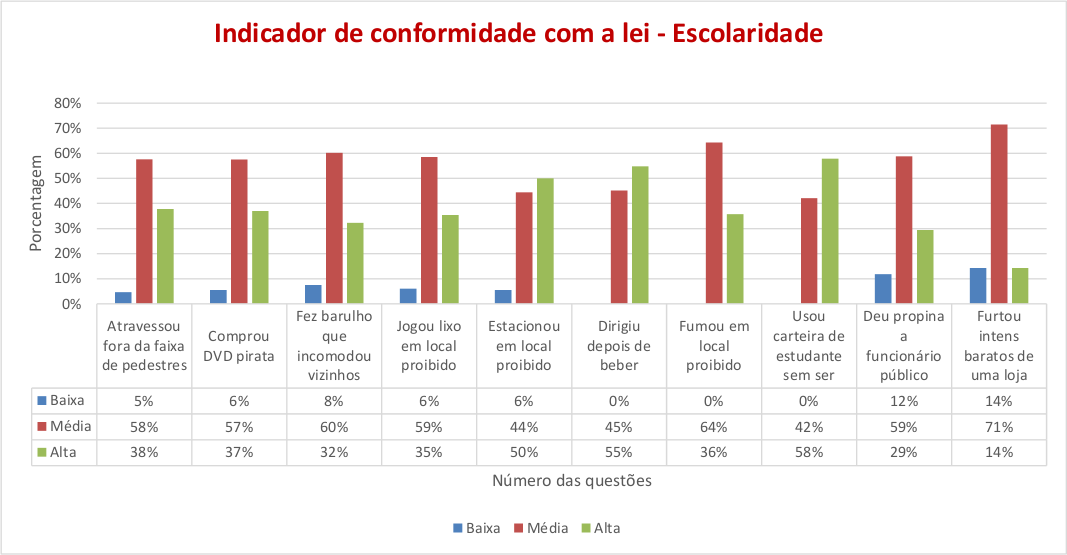
\includegraphics[scale=0.5]{Conformidade-escolaridade.png}
	\end{center}
	\ABNTEXchapterfont\small{Fonte: elaborado pelo autor - agosto de 2015}
	\label{Conf_escola}
\end{grafico}
\FloatBarrier
\par
O grau de instrução também mostra um dado interessante, pois ao contrário de que muita gente pensa, os menos favorecidos são so que menos descumprem a lei.
\begin{grafico}[!htpb]
	\caption{Indicador de Conformidade - Renda - NATAL, 2015}
	\begin{center}
		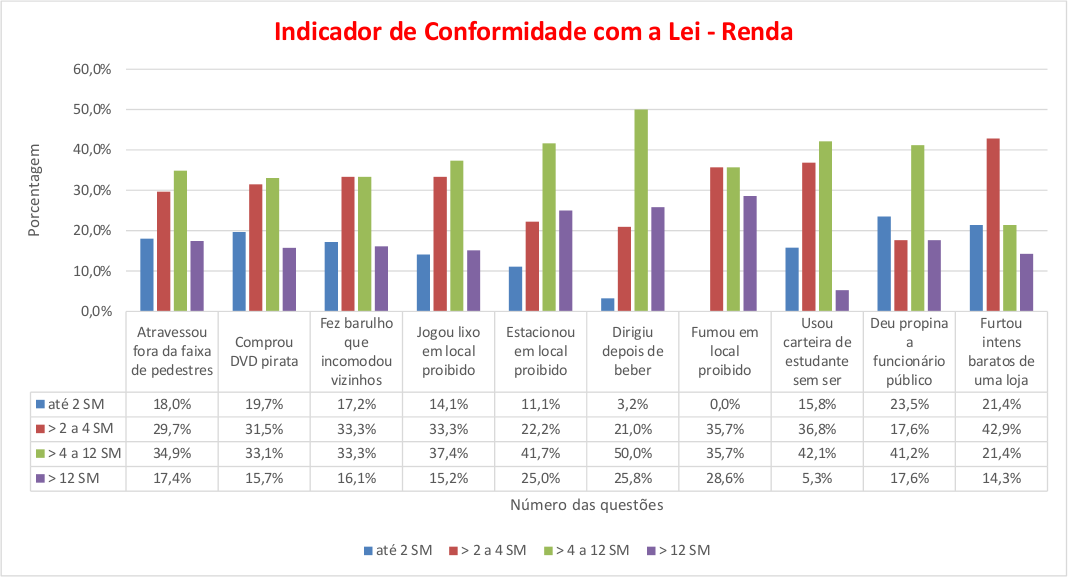
\includegraphics[scale=0.5]{Conformidade-renda.png}
	\end{center}
	\ABNTEXchapterfont\small{Fonte: elaborado pelo autor - agosto de 2015}
	\label{Conf_renda}
\end{grafico}
\FloatBarrier
\par
Já a renda ficou concentrada na classe média os maior violadores das regras. Novamente os menos favorecidos financeiramente são os que menos violam as leis.
\par
Concluindo, de acordo com os gráficos 9 a 12, o perfil de quem mais transgride as normas é:\\
sexo masculino \textbf{E} faixa de idade 15 a 34 anos \textbf{E} grau de instrução - ensino médio \textbf{E} renda maior que 4 até 12 SM
\begin{foto}[!htpb]
	\caption{\label{Foto10}O comércio informal em Natal - Bairro do Alecrim}
	\begin{center}
		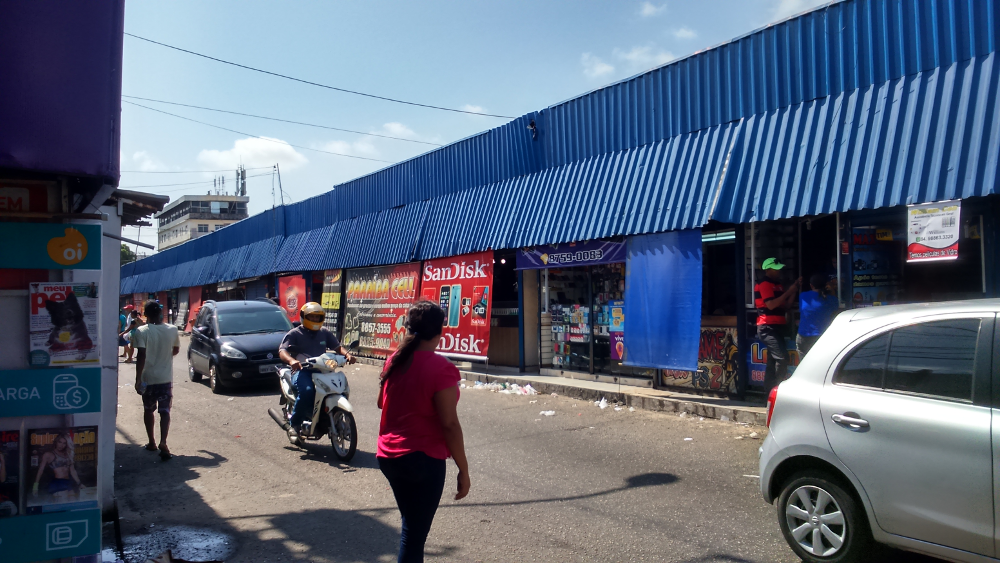
\includegraphics[scale=0.20]{alecrim.png}
			\end{center}
	\ABNTEXchapterfont\small{Fonte: Produzida pelo autor - agosto de 2015}
\end{foto}
\FloatBarrier
\begin{foto}[!htpb]
	\caption{\label{Foto11}O “paradigma de Zimbardo” - Quadra de esportes abandonada na Av. Ayrton Senna em Natal}
	\begin{center}
		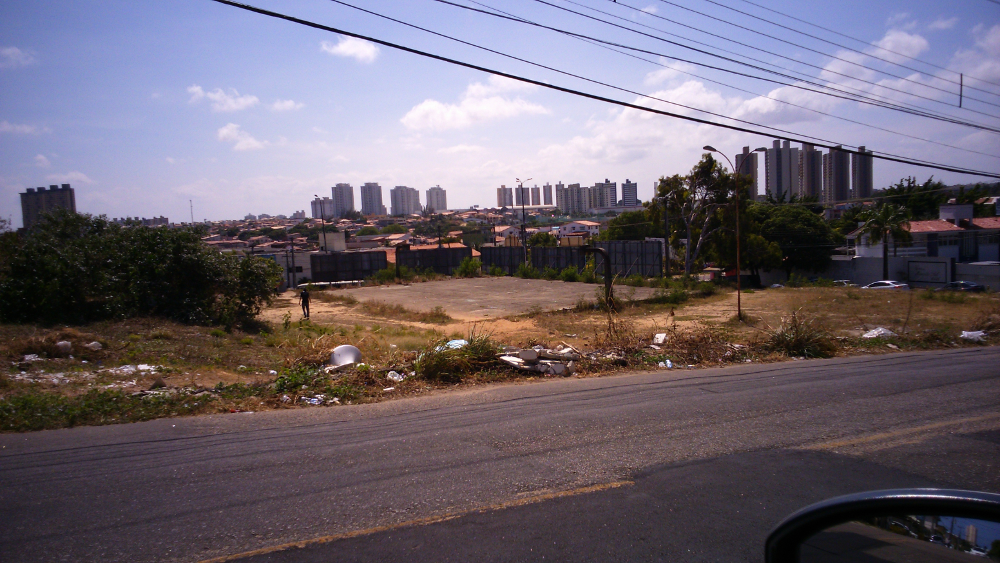
\includegraphics[scale=0.42]{ayrton-senna.png}
	\end{center}
	\ABNTEXchapterfont\small{Fonte: Produzida pelo autor - agosto de 2015}
\end{foto}
\FloatBarrier
\section{Índice de Legitimidade}
Outro índice que vale a pena ser mostrado é o de legitimidade, onde os entrevistados responderam perguntas sobre sua percepção a respeito das leis e das autoridades. Assim, foram também reunidas as respostas “Concorda muito” e “Concorda um pouco” e seu resultado comparado com o número total de entrevistados (gráfico 13).
\begin{grafico}[!htpb]
	\caption{Indicador de legitimidade - Geral - NATAL, 2015}
	\begin{center}
		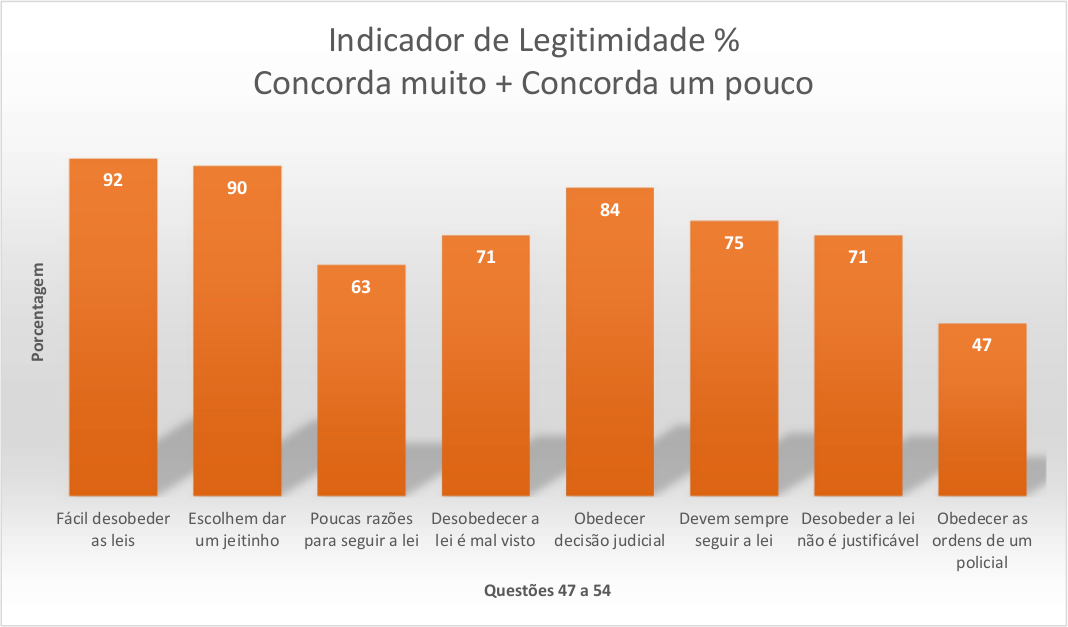
\includegraphics[scale=0.55]{Legitimidade_geral.png}
	\end{center}
	\ABNTEXchapterfont\small{Fonte: elaborado pelo autor - agosto de 2015}
	\label{Leg_geral}
\end{grafico}
\begin{grafico}[!htpb]
	\caption{Indicador de legitimidade - Sexo - NATAL, 2015}
	\begin{center}
		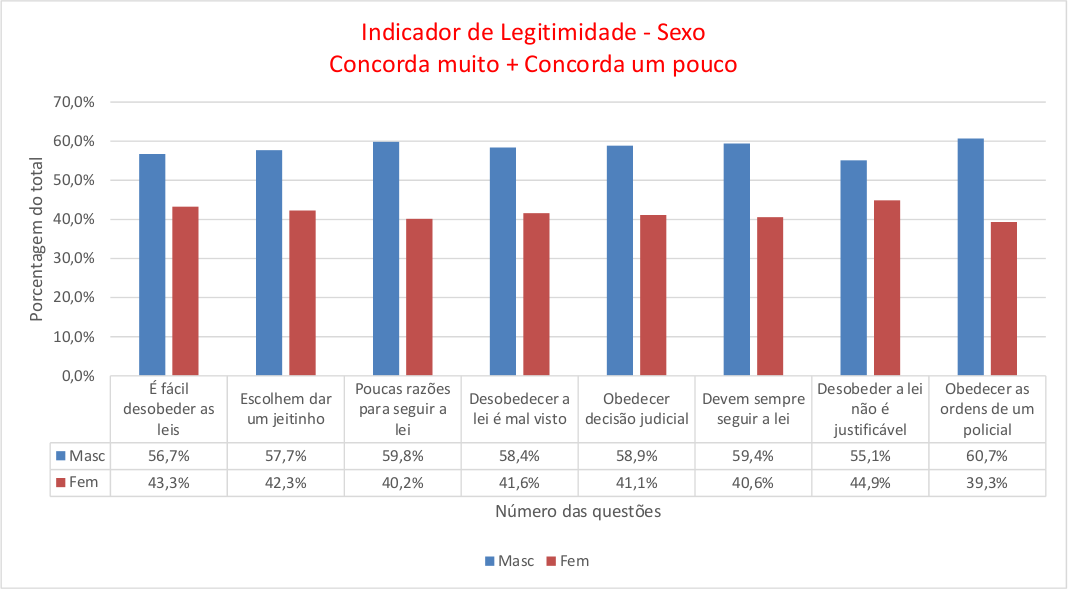
\includegraphics[scale=0.5]{Legitimidade-sexo.png}
	\end{center}
	\ABNTEXchapterfont\small{Fonte: elaborado pelo autor - agosto de 2015}
	\label{Leg_sexo}
\end{grafico}

\begin{grafico}[!htpb]
	\caption{Indicador de legitimidade - Faixa de idade - NATAL, 2015}
	\begin{center}
		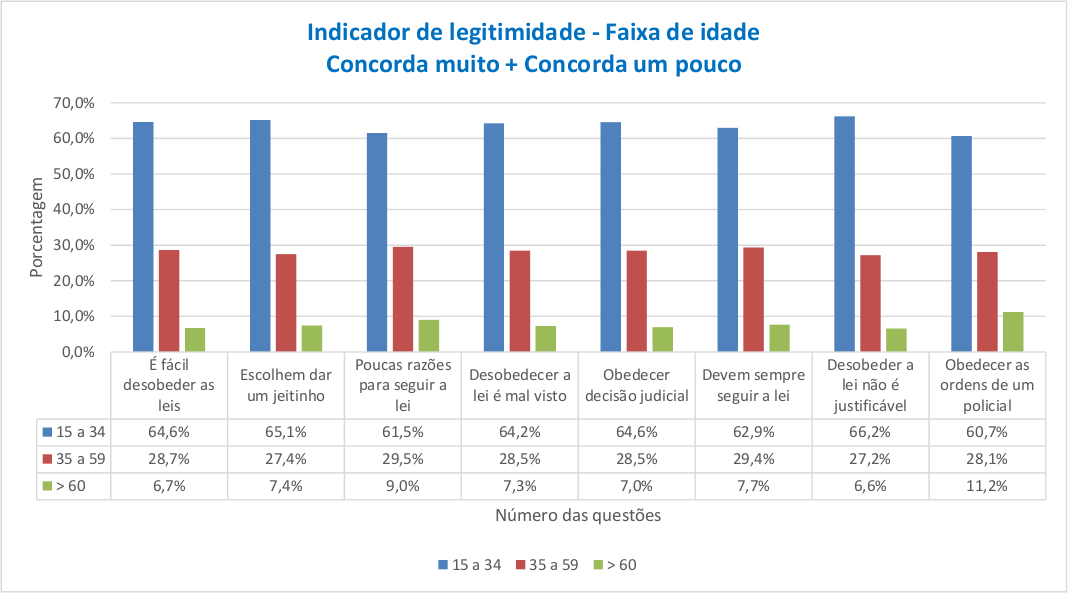
\includegraphics[scale=0.5]{Legitimidade-idade.png}
	\end{center}
	\ABNTEXchapterfont\small{Fonte: elaborado pelo autor - agosto de 2015}
	\label{Leg_idade}
\end{grafico}
\begin{grafico}[!htpb]
	\caption{Indicador de legitimidade - Grau de instrução - NATAL, 2015}
	\begin{center}
		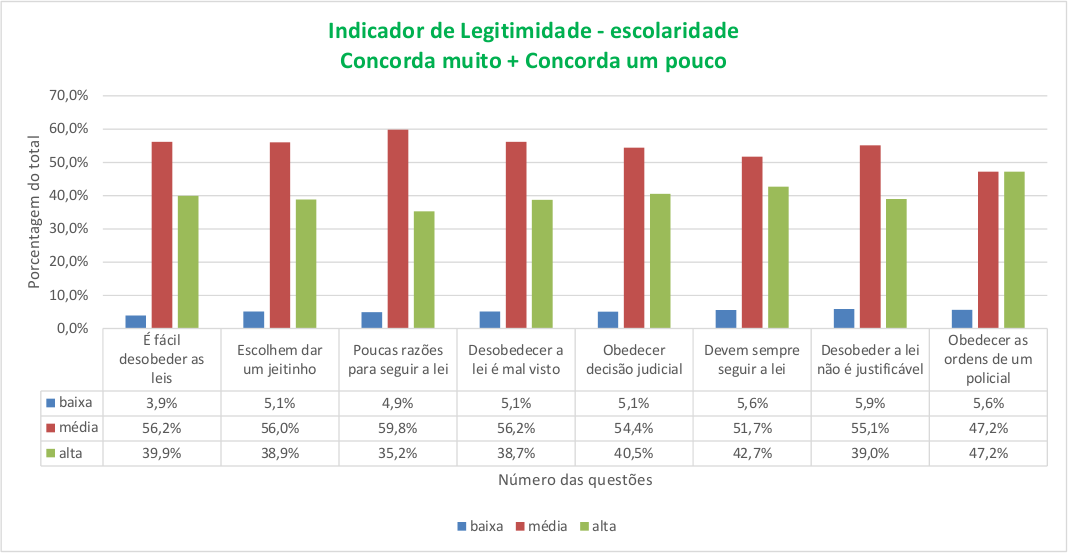
\includegraphics[scale=0.5]{Legitimidade-escolaridade.png}
	\end{center}
	\ABNTEXchapterfont\small{Fonte: elaborado pelo autor - agosto de 2015}
	\label{Leg-escola}
\end{grafico}
\begin{grafico}[!htpb]
	\caption{Indicador de legitimidade - Renda - NATAL, 2015}
	\begin{center}
		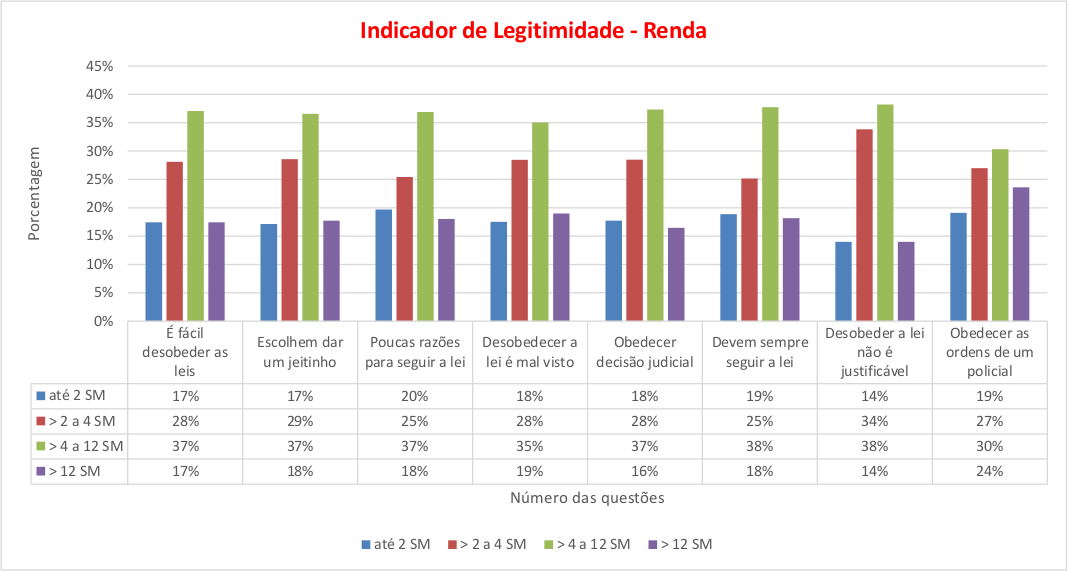
\includegraphics[scale=0.5]{Legitimidade-renda.png}
	\end{center}
	\ABNTEXchapterfont\small{Fonte: elaborado pelo autor - agosto de 2015}
	\label{Leg-renda}
\end{grafico}
\par
Obtém-se portanto a maioria que concorda com as afirmações:
Sexo masculino \textbf{E} idade 15 a 34 anos \textbf{E} grau de instrução - ensino médio \textbf{E} renda maior que 4 até 12 SM.
\par
Traduzindo para as questões é uma pessoa que concorda que é fácil desobedecer leis no Brasil, sempre que possível as pessoas escolhem dar um jeitinho ao invés de seguir a lei, acredita que existem poucas razões para uma pessoa seguir a lei no Brasil, tem consciência que alguém de desobedece a lei é mal visto pelas outras pessoas, deve-se obedecer as ordens judiciais, dos policiais e obedecer a lei de modo geral, mesmo que discorde delas e, que desobedecê-las raramente é justificável.
\par
Interessante que a única coisa que muda do grupo de gráficos 9 a 12 e 14 a 17 é a faixa de idade. Nota-se também que a renda é um fator preocupante para o primeiro grupo pois existe uma faixa entre 4 até 12 SM que mais comete irregularidades. Será o sentimento de impunidade que o dinheiro traz?
\par
Considerando que o IPCL-Natal é um índice que mediu todo o universo de entrevistados, uma outra análise interessante e que fica como sugestão se alguém quiser expandir o presente trabalho, é realizar esse cálculo usando como filtros as quatro variáveis acima de forma a obter-se um IPCL-Natal estratificado (IPCL-Natal-sexo, IPCL-Natal-idade, IPCL-Natal-instrução, IPCL-Natal-renda). Alguns resultados podem ser surpreendentes.

\chapter{Elaboração da Análise SWOT}
\section{Conceito de Análise SWOT}
\lettrine[lines=2, lhang=0.33, loversize=0.25]{A} {análise} SWOT é um procedimento desenvolvido na segunda metade do século passado com o objetivo de fazer o mapeamento das
forças e fraquezas (parte interna) e oportunidades e ameaças (parte externa) de uma empresa. Tratava-se de um procedimento organizacional
e voltado para a área administrativa. Todas as grandes empresas possuem sua análise SWOT de forma a garantir uma visão consolidada
de sua posição no mercado\footnote{N.A. Vide exemplo em: \href{http://www.freeswotanalysis.com/aerospace-airline/642-embraer-swot-analysis.html}{Análise SWOT Embraer} - acesso em:24.7.2015}.
\par
Entretanto esse conceito encontrou aplicabilidade em outros campos. Com o surgimento do neoliberalismo, o modelo de administração gerencial do Estado e a administração voltada a resultados, onde a população não é mais um usuário mas sim um cliente dos serviços públicos, a análise SWOT se prestou muito bem para diagnosticar a eficiência da máquina estatal. Até a nível pessoal ela pode ser usada exatamente para que o indivíduo
tenha um diagnóstico de possíveis problemas que enfrentará ao longo de sua vida.

\begin{figure}[!h]%NBR 14724:2011 item 5.8
	\caption{Matriz SWOT}
	\begin{center}
	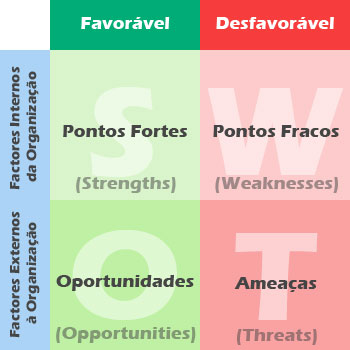
\includegraphics[scale=0.7]{matriz-swot.jpg}
	\end{center}
	\ABNTEXchapterfont\small{Fonte:\href{http://blog.luz.vc/wp-content/uploads/2013/10/matriz-swot.jpg}{Matriz SWOT} - acesso em 1.7.2015}
	\label{swot}
\end{figure} 
Como mostra a figura acima, a análise SWOT é divida em quatro setores, como explicado:
\par
\textbf{Forças:} Significa, no âmbito interno da organização (privada ou pública), as forças que ela possui para se firmar no mercado (marca reconhecida,
respeitabilidade, credibilidade, capital, conhecimento, tecnologias, etc.). De acordo com \citeonline[p. ~151]{Matos} as forças são “Recursos e habilidades de que dispõe a organização para explorar as oportunidades e minimizar as ameaças”. Na análise me tela, são as variáveis que a Administração Pública tem controle ou delas pode se aproveitar.
\par
\textbf{Fraquezas:} “As fraquezas são consideradas deficiências que inibem a capacidade de desempenho da
organização e devem ser superadas para evitar falência da organização” \citeonline[p. 52]{Matos}, (no presente caso, o fracasso da implementação da Tolerância Zero). Considerando que a Administração Pública possui algum controle sobre essas variáveis, as mesmas devem ser minimizadas ou se possível, eliminadas.
\par
\textbf{Oportunidades:} São situações, tendências ou fenômenos externos, atuais ou potenciais, que podem
contribuir para a concretização dos objetivos estratégicos. A Administração pode (e deve) se apropriar delas para alcançar seus objetivos.
\par
\textbf{Ameaças:} São fatores externos que fogem ao controle da Administração Pública, mas que podem ser identificados e classificados como imediatos ou potenciais, de forma a hierarquizar de forma a resolvê-las de plano ou preparar com antecedência estratégias para seu enfrentamento.


\section{Análise SWOT para o Município de Natal}
\lettrine[lines=2, lhang=0.33, loversize=0.25]{C}{om} base nas respostas e do cruzamento dos dados do questionário submetido do  IPCL-Natal e a própria percepção do autor em mais de dezoito meses de pesquisa, foi
construída uma análise SWOT sobre o município
de Natal que servirá de subsídio para verificar as dificuldades para a implantação de uma política de tolerância zero
na capital potiguar. Em cada item, são comentadas também algumas possíveis sugestões para resolver/minimizar os problemas:

\subsection{Forças - \textit{Strenghts}}
\hypertarget{S1}{} 
\paragraph*{\textbf{1. Confiança em algumas instituições:}} Apesar de uma significativa maioria ter-se pronunciado não confiar em nenhuma instituição (pergunta 55) nota-se também que  uma significativa parcela acredita no Ministério Publico, Forças Armadas e Igreja. A polícia entretanto encontra-se desacreditada (veja gráfico 6). Cabe a essas instituições modificar essa visão da sociedade natalense.\\
\hypertarget{S2}{}
\paragraph*{\textbf{2. Polícia bem equipada:}} Percebe-se que em termos de equipamentos disponibilizados, a Polícia Militar do RN está razoavelmente bem equipada. Entretanto nota-se que a maioria são equipamentos letais (pistolas, escopetas, metralhadoras, etc.). Da mesma forma que uma polícia bem equipada é necessária, os equipamentos devem ser aperfeiçoados. Há 15-20 anos atrás os bandidos da cidade do Rio de Janeiro ironizavam o armamento usado pela polícia (revólver calibre 38) enquanto eles usavam pistolas 9mm e fuzis AR-15; hoje em dia enquanto a Amazon pretende usar drones para entregar livros, os traficantes pensam em usá-los para entregar drogas. O crime não pode estar um passo a frente da polícia. O uso de equipamentos com menor potencial ofensivo também deve ser implantado, pois a polícia nem sempre se depara com bandidos. A truculência policial deve ser reprimida (veja a definição de \hyperlink{poder}{Poder}).
\hypertarget{S3}{}
\paragraph*{\textbf{3. Pessoal treinado para missões em campo:}} O treinamento que a polícia tem é no sentido corretivo e de confronto. Para esse tipo de operação, entende-se que está bem preparada, entretanto ainda prevalece o conceito que todo mundo é suspeito até que prove o contrário(?). A polícia deve estar apta a lidar com a população também, que na verdade é seu maior cliente.
\hypertarget{S4}{}
\paragraph*{\textbf{4. Município com várias universidades:}} o município de Natal tem uma ótima infraestrutura educacional de nível superior, proporcionando oportunidades para a população carente através de sistemas de cotas e políticas do governo federal. Os preços praticados pelas instituições particulares são inferiores aos das regiões sul/sudeste. Programas de inclusão através de cotas ou bolsas são relativamente bons.
\hypertarget{S5}{}
\paragraph*{\textbf{5. Baixa industrialização:}} Natal possui pouca expressão em termos de industrialização se comparada a Fortaleza e Recife. Isso possui aspectos positivos e negativos: positivo visto que a poluição industrial é menor (o ecossistema presente na capital potiguar pode ser classificado com bem sensível a agressões poluentes), em caso de crise não existe um desemprego maciço com grandes demissões; o negativo é a falta de oportunidades que obriga os mais jovens a migrarem em busca de emprego. Dessa forma, entende-se como uma força do município.
\hypertarget{S6}{}
\paragraph*{\textbf{6. Excelente clima:}} Natal possui um excelente clima, sem variações bruscas de temperaturas e uma qualidade do ar considerada ótima. Nesse quesito, a qualidade de vida em Natal é uma das melhores do mundo. Isso é um convite para que o Estado propicie condições para que
pessoas/entidades de alto nível migrem para cá.\\

\subsection{Fraquezas - \textit{Weakness}}
\hypertarget{W1}{}
\paragraph*{\textbf{1. Percepção da população sobre o grau de dificuldade na implantação de uma política de tolerância zero (pergunta 56 do questionário):}} 71\% dos entrevistados classificou com um grau de dificuldade maior ou igual a sete esse grau de dificuldade. Sem dúvida é com razão tal pensamento, visto ser claro que a impunidade e o descaso das autoridades estão presentes no município. Casos como a tolerância zero para embriagues ao volante devem ser expandidos para outros delitos. Nesse sentido, veja veja o subitem \hyperlink{B1}{subitem B1} da entrevista com o Cap. Styvenson 
\hypertarget{W2}{}
\paragraph*{\textbf{2. Inteligência da polícia despreparada:}} Não existe um setor de inteligência expressivo para prever/controlar ações criminosas. Considerando o treinamento da polícia voltado para o confronto, de forma corretiva somente, não existe uma preocupação em montar uma estrutura preditiva na polícia. Segundo informações verbais recebidas, o material de treinamento da polícia militar é dos anos 70 (regime ditatorial). Não deve ser menosprezado que o crime possui seu setor de inteligência, principalmente as facções criminosas e com a vantagem que não estão
sujeitos a realização de concursos públicos e/ou licitações para se equipar. Sobre um exemplo de inteligência, veja o \hyperlink{B7}{subitem B7} da entrevista com o Cap. Styvenson.
\hypertarget{W3}{}
\paragraph*{\textbf{3. Turismo sem controle:}} Não existe um controle de quem desembarca aqui. O turismo é uma atividade predatória se não for bem controlada, pois o turista não tem nenhum compromisso com o município. Ele vem, usufrui e vai embora. Outro grande problema é o turismo sexual instalado na cidade e que felizmente parece ter arrefecido de alguns anos para cá. Sobre o turismo, é interessante mostrar uma frase do escritor Ronaldo Bressane\footnote{N.A. Disponível em \href{http://entretenimento.uol.com.br/noticias/redacao/2015/07/04/violencia-em-paraty-o-que-roberto-saviano-temeria-para-nao-vir-a-flip.htm}{Violência em Paraty-RJ} - acesso em 1.7.2015}, escritor que morou na cidade turística de Paraty – Rio de Janeiro e considerada a terceira mais violenta do estado: “Todo tempo tem troca de pipoco em uma rua entre a Mangueira e a Ilha das Cobras (...) Paraty é fruto do espólio. Espólio do ouro, dos escravos, do café e \textbf{agora do turismo}”(grifo do autor).
\hypertarget{W4}{}
\paragraph*{\textbf{4. Corrupção:}} Natal (e o RN) ainda são vitimas do coronelismo de forma velada, com um oligopólio de famílias se alternando no poder e com isso favorecendo o clientelismo, o nepotismo (cruzado ou não), o favoritismo e outras formas de agir não condizentes com um estado ético. O mandonismo ainda permeia por aqui, o “você sabe com quem está falando?” é corriqueiro. Cabe aos órgãos não governamentais a tentativa de mudar essa situação e, nessas horas, mostrar que a lei é para todos.
\hypertarget{W5}{}
\paragraph*{\textbf{5. Falta de confiança da população nas instituições:}} Conforme pode ser verificado na questão sobre confiança nas instituições, 39\% dos entrevistados não confiam em nenhuma instituição. Entende-se que na verdade existe uma descrença na eficiência dessas instituições em resolver os problemas da população. Isso revela-se perigoso, pois a população pode tomar em suas mãos a resolução de problemas.
\hypertarget{W6}{}
\paragraph*{\textbf{6. Ouvidorias “surdas”:}} Nota-se frequentemente o reclamo da população sobre a “surdez” das ouvidorias. Como comprovação, o autor desse trabalho, no primeiro semestre de 2015, enviou denúncias ao Ministério Público do Estado do RN, Banco Central do Brasil e Corpo de Bombeiros de Natal. Dos dois primeiros recebeu respostas totalmente diversas à denúncia e do último sequer recebeu resposta. Tentou
ainda obter dados atualizados diretamente de órgão públicos do RN sem conseguir uma única resposta.
\hypertarget{W7}{}
\paragraph*{\textbf{7. Soluções paliativas – ações corretivas:}} O agir das instituições responsáveis pela segurança pública se dá no contexto corretivo, ou seja, após o fato já ter se consumado. Devido ao fraco desempenho do setor de inteligência da polícia, não há como atuar preventivamente. Cabe urgentemente reavaliar e modernizar  essa área vital, através de uma maciça capacitação do pessoal existente e contratação de novos profissionais. A parceria com as universidades deve ser feita para o uso de novas tecnologias (Observatório das Metrópoles da UFRN, por exemplo).
\hypertarget{W8}{}
\paragraph*{\textbf{8. Falta de efetivo nas polícias:}} Muitos anos sem concurso público praticamente sucatearam a polícia do Rio Grande do Norte. O atual governo está tentando reaparelhar o efetivo da polícia, mas isso é uma ação de longo prazo, pois requer capacitação e treinamento. Não se deve permitir a instalação desses hiatos, mas sim fazer com que a reposição de pessoal seja um contínuo ao longo das administrações.
\hypertarget{W9}{}
\paragraph*{\textbf{9. Sistema penitenciário falido:}} Enquanto Natal e o Rio Grande do Norte se orgulham de possuir um estádio de futebol de primeiro mundo, um aeroporto de utilidade duvidosa e outras obras faraônicas, o sistema penitenciário está falido, com cadeias e presídios superlotados, verdadeiros depósitos de gente. A promiscuidade e a corrupção estão instaladas nesses locais. Em visita ao presídio de Alcaçus em Nísia Floresta, o então Ministro do STF Joaquim Barbosa definiu como “um queijo suíço” dada a grande quantidade de túneis existentes. Acredita-se que só a verba gasta na construção do Arena das Dunas, seria possível resolver o problema prisional do Estado. Ver as \hyperlink{CA1}{Considerações Adicionais}
\hypertarget{W10}{}
\paragraph*{\textbf{10. Alta desigualdade social:}} como mostrado nas fotos 4 e 5, a desigualdade social só muda de endereço. Não é necessário ser uma megalópole como São Paulo para que isso ocorra. A brusca mudança de um IDHM de mais de 0,9 para um em torno de 0,4 somente atravessando uma rua sem dúvida é impactante. O desenvolvimento de políticas de valorização dessa população deve ser incentivado. Infelizmente existe em nosso meio um grande preconceito contra esse tipo de população. A pessoa que não teve oportunidades é taxado de vagabundo pelas classes mais favorecidas. Entretanto uma ressalva deve ser feita: o fato de uma pessoa ser pobre, ter nascido no lugar errado, crescido na miséria, em uma família desestruturada, não teve uma estrutura escolar formadora e não conviveu com pessoas do bem não deve ser usado como justificativa para o cometimento de ações criminosas. Isso é uma fábula social muito em voga atualmente, onde a culpa por isso é jogada para o descaso da sociedade. Veja sobre isso na definição de desvios por \hyperlink{Gid1}{Giddens}.
\hypertarget{W11}{}
\paragraph*{\textbf{11. Sistemas de ensino básico e médio ruins:}} Salários baixos, desmotivação, violência, frequentes furtos e roubos, depredação do patrimônio público, deficit de pessoal, esse é um raio X da educação em Natal nos níveis básico e médio. De nada adianta uma excelente estrutura de nível superior implantada no município se a educação de base não satisfaz o mínimo necessário. Em recente depoimento ouvido no campus da UFRN, o autor soube que apenas 10\% dos ingressantes no curso básico de Ciência e Tecnologia conseguem completar o período inicial de dois anos, visto a deficiência para acompanhar as disciplinas do campo de exatas. Ainda nesse sentido, vide o gráfico 1 que mostra ser exatamente nesse período da vida que deve existir uma maior intervenção do Estado na vida das crianças. Ainda sobre isso, veja o \hyperlink{B3}{subitem B3} da entrevista com o Cap. Styvenson.
\hypertarget{W12}{}
\paragraph*{\textbf{12. Cidade abandonada:}} Ruas e calçadas mal conservadas, prédios abandonados, sujeira, região central com ocupação desordenada e poluição visual. Este é um raio-X do município de Natal. Um dos princípios basilares da política de tolerância zero é o fim do descaso da administração pública para com o município. Imóveis sem destino definido como o hotel BRA na via costeira, o hotel Reis Magos na praia dos Artistas, a região de Cidade Alta, Ribeira e Alecrim sem o mínimo ordenamento urbano trazem a visão de pouca importância das autoridades para com o município (vide o Anexo C). E o paradigma de Zimbardo novamente se faz presente...
\hypertarget{W13}{}
\paragraph*{\textbf{13. Empoderamento da polícia:}} Quando da implantação da tolerância zero em New York foram relatados casos de abuso de autoridade por parte da polícia, principalmente em relação as minorias. É de se esperar que o mesmo ocorra por aqui em caso da implantação de uma política de tolerância zero, o que deverá ser imediatamente averiguado e punido. As corregedorias deverão estar em contínuo estado de atenção durante a execução da política. Veja o \hyperlink{B15A}{subitem B15 (final) e B16} da entrevista com o Cap. Styvenson.\\

\subsection{Oportunidades - \textit{Opportunities}}
\hypertarget{O1}{}
\paragraph*{\textbf{1. Percepção das pessoas sobre a desobediência às leis:}} 71\% das pessoas entrevistadas disseram que “concordam muito” ou “concordam um pouco”  para a pergunta 50: “Alguém que desobedece a lei é mal visto pelas outras pessoas”. Trata-se de um bom sinal da percepção da população sobre pessoas que cometem atos ilegais. Resta saber se isso se aplica ao próprio núcleo familiar de quem respondeu (dois pesos, duas medidas). Sobre a percepção das pessoas sobre o poder Judiciário, pergunta 51: “Se o Juiz decide que uma pessoa pague à outra uma quantia, ela tem a obrigação moral de pagar mesmo que discorde da decisão” verifica-se que 81\% dos entrevistados concordam muito ou concordam um pouco. Isso reforça a tese da confiança no judiciário, conforme mostrado na questão 55.
\hypertarget{O2}{}
\paragraph*{\textbf{2. Estrita obediências às leis:}}As perguntas 52 “As pessoas devem seguir a lei mesmo quando a lei é contraria ao que elas acreditam que é certo” e 53 “Desobedecer à lei raramente é justificável” mostram que grande parcela dos entrevistados (75\% e 71\%) possuem um bom nível de obediência às leis. Isso deve ser tomado como um facilitador na implantação da politica de tolerância zero, pois terá apoio de grande parte da população.\hyperlink{B2}{Veja o subitem B2} do Anexo B.
\hypertarget{O3}{}
\paragraph*{\textbf{3. Criação de uma “police smarter, not harder”:}} Valorizar, capacitar e equipar a inteligência da polícia, no sentido de haver um
completo mapeamento do crime no município e intensificar ações nesses “pontos negros”. É fato conhecido que na hierarquia do crime (o topo são
os assaltantes de bancos), que os delitos de menor poder ofensivo ocorrem dentro de um mesmo território. O uso maciço de estatísticas e
técnicas de geoprocessamento deve ser incentivado para prever e coibir essas ações\footnote{N.A. Nesse sentido: \href{http://www.ibm.com/smarterplanet/us/en/leadership/memphispd/assets/pdf/IBM_MemphisPD.pdf}{Análise preditva}}. Nas Considerações adicionais será mostrado o exemplo de São José dos Campos - SP.
\hypertarget{O4}{}
\paragraph*{\textbf{4. Unificação das polícias:}} Assunto que vem sendo amplamente debatido há muitos anos, a unificação das polícias significaria na criação de um plano único de carreira que valorize o profissional por meritocracia. O modelo americano deve ser analisado e cogitado. A criação de mecanismos para facilitar o acesso desses profissionais à educação deve ser incentivado. A polícia ainda conserva o “ranço” da ditadura militar. Uma experiencia que amenizou a visão da sociedade sobre a polícia, foi a retirada, em alguns estados das regiões sul/sudeste, o termo “militar” de sua identificação.
\hypertarget{O5}{}
\paragraph*{\textbf{5. A cidade intelectual:}} Como dito no item Forças, o baixo grau de industrialização aliado ao excelente clima e a existência uma uma boa rede de ensino superior pode fazer com que o município, nos moldes do Vale do Silício nos EUA, “pule” a etapa da industrialização e parta para uma fase intelectual. A ideia é convidar e incentivar o maior número de institutos de pesquisa, tanto do setor público como privado, nacionais ou internacionais, a se instalarem aqui. Natal é um excelente lugar para o exercício do ócio criativo. A população irá ganhar com a geração de empregos na área de serviços e aquecimento do comércio, visto o bom poder aquisitivo dessas pessoas.
\hypertarget{O6}{}
\paragraph*{\textbf{6. Aumento das ações sociais na periferia:}} Sem dúvida a aumento/criação de ações sociais na periferia em muito contribuiriam para diminuir a desigualdade social no município. Fixar o trabalhador em seu bairro deve ser uma das metas, o empreendedorismo deve ser incentivado, a criação de um banco municipal para financiamento de microempreendedores individuais com facilidades de pagamento e constante monitoramento do uso do dinheiro e de outro lado a saturação de ações policiais nos bairros mais violentos.
\hypertarget{O7}{}
\paragraph*{\textbf{7. Incentivo ao planejamento familiar:}} A criação de uma política pública de planejamento familiar, para a população, com o fim do conceito que “onde comem 5, comem 6, 7, 8...” e que os filhos são tidos porque Deus assim quis, deve ser incentivado. O acesso a meios contraceptivos deve ser facilitado e até premiado. A laicidade do Estado deve prevalecer em detrimento de conceitos religiosos.
\hypertarget{O8}{}
\paragraph*{\textbf{8. Polícia de bairro:}} Em seu livro “Fixing Broken Windows”, (sem tradução para o vernáculo), os autores defendem a prevenção baseada na comunidade. Assim eles entendem que a criação de polícias de bairro, sempre com os mesmos policiais fazendo a ronda a pé, geram um sentido de cumplicidade entre a população residente e a polícia. Existem algumas críticas à esse modelo, pois o mesmo mostrou-se discriminatório por eleger como “potencialmente suspeita” qualquer pessoa desconhecida que adentre o território\footnote{N.A. Adiante será discutida a plataforma de governo do atual governador do RN no quesito Segurança Pública, que prevê esse tipo de ação}.
\hypertarget{O9}{}
\paragraph*{\textbf{9. Maior controle sobre crianças/adolescentes:}} Toda criança ou adolescente em idade escolar deve ser questionado (polícia ou guarda municipal) a qualquer momento pelas autoridades sobre seu horário de aulas e caso seja constatada a falta à escola, encaminhado para o conselho tutelar o qual irá contatar os pais e averiguar o por quê da ausência à aula e se for o caso, tomar medidas corretivas. Em sua coluna na revista Veja, o economista Cláudio Moura e Castro  menciona que “Ao serem divulgados os resultados das primeiras
provas do ENEM, um grande grupo educacional encomendou uma pesquisa com os alunos das dez melhores escolas do Brasil. Pois não é que eram todas parecidas? Chamava a atenção o fato de serem muito rígidas na disciplina. Ou seja, nada de bagunça. E entre as instituições públicas, com sua disciplina severa, os colégios militares tem ótimo desempenho” \citeonline[p. ~20]{Veja}. Outra medida a ser incentivada é o turno único de estudo bem como atividades complementares obrigatórias aos sábados. Nesse sentido veja a parte final do \hyperlink{B3}{subitem B3} da entrevista com o Cap. Styvenson.\\

\subsection{Ameaças - \textit{Threats}}
\hypertarget{T1}{}
\paragraph*{\textbf{1. Desobediência civil:}} As repostas das questões 47 - É fácil desobedecer as leis no Brasil: 92\% concordam, 48 - Sempre que possível as pessoas escolhem dar um “jeitinho” ao invés de seguir a lei: 90\% concordam e 49 - Existem poucas razões para uma pessoa seguir a lei no Brasil: 63\% concordam demostram o total descrédito da população em relação ao cumprimento das leis no Brasil e a falta de punição por parte do Estado. Sobre a desobediência civil, Thoreau faz algumas interessantes perguntas:
\begin{citacao}
	Leis  injustas  existem:  devemos  contentar-nos  em  obedecer  a  elas  ou  esforçar-nos  em corrigi-las, obedecer-lhes até triunfarmos ou transgredi-las desde logo? Num governo como este, os homens geralmente pensam que devem esperar até que a maioria seja persuadida a alterá-las. Pensam que, se resistissem ao governo, o remédio seria pior que o mal. Mas é culpa do próprio governo que o remédio seja, efetivamente, pior que o mal. É ele que o torna pior. Por que ele não está  mais  apto  a  antecipar  e  proporcionar  a  reforma?  Por  que  não  trata  com  carinho  sua  sábia minoria?  Por  que  suplica  e  resiste  antes  de  ser  ferido?  Por  que  não  encoraja  seus  cidadãos  a prontamente apontarem seus defeitos e a agirem melhor do que ele lhes pede? \cite[p.~5]{Thoreau}
\end{citacao}
Maiores referências sobre a desobediência civil serão feitas nas \hyperlink{CA2}{Considerações Adicionais}. Ir para \hyperlink{Conf1}{Índicador de Conformidade}.
\hypertarget{T2}{}
\paragraph*{\textbf{2. Falta de confiança nas instituições:}} Novamente volta-se à pergunta 58 - Em qual (is) dessas instituições você confia, antes vista como força e agora como ameaça devido a grande maioria ter dito não acreditar em nenhuma das instituições. Tal opinião, pode se inferir, repete-se a nível nacional, com os tantos escândalos divulgados na mídia em vários setores de onde se esperava um comportamento ético. 
Ainda como comprovação, tem-se a questão 54 - Se um policial pede para uma pessoa fazer algo, ela deve fazer mesmo que discorde do policial com 54\% de discordância dos entrevistados.
\hypertarget{T3}{}
\paragraph*{\textbf{3. Implantação do crime organizado:}} Como já foi mencionado, onde existe a desordem, o descaso (ou impotência) das autoridades para “arrumar a casa” abre-se a oportunidade do crime se instalar. Nos mesmos moldes de Diadema, onde o trafico elegeu a cidade para se instalar, organizações criminosas como o PCC estão elegendo Natal para sediar suas ações criminosas na região. Ainda há tempo hábil para corrigir isso, pois Natal não possui uma densidade populacional tão grande como seus vizinhos (Fortaleza e Recife).
\hypertarget{T4}{}
\paragraph*{\textbf{4. Resolução de divergências pela violência:}} Infelizmente ainda existe esse tipo de cultura no município talvez causada em grande parte pela desconfiança na capacidade das instituições públicas responderem rapidamente às demandas.  Nesse sentido, \citeonline[p. ~23]{Weber}: “Uma relação social denomina-se \textit{luta} quando as ações se orientam pelo propósito de impor a própria vontade contra a resistência do ou dos parceiros”.A facilitação do acesso a justiça (pequenas causas) talvez seja uma saída viável para minimizar o problema, com a inclusão dos centros de estágio jurídico das universidades. Entretanto, essa cultura não é resolvida no curto prazo e deve ser alvo de uma maciça conscientização/educação da população em repreender essas ações.
\hypertarget{T5}{}
\paragraph*{\textbf{5. População fazendo justiça com as próprias mãos:}} Trata-se de um flagrante desrespeito às instituições, mas é uma cultura que infelizmente está se alastrando pelo país e amplamente noticiada pela mídia. Em síntese, quando o Estado falha na prevenção, no acompanhamento e na correção de delitos, a população se revolta e de modo irracional aplica o seu entendimento de justiça\footnote{N.A. Nesse sentido: \href{http://tribunadonorte.com.br/noticia/suspeito-de-estupro-a-linchado-e-morto-por-moradores-em-felipe-camara-o/323492?utm_campaign=noticias&utm_source=20150903}{Linchamento em Natal} - acesso em: 4.9.2015}. Os conceitos de que “a polícia prende  e o juiz solta” e “bandido bom é bandido morto” devem ser extirpados do imaginário popular.
\hypertarget{T6}{}
\paragraph*{\textbf{6. Implantação de uma cultura do medo:}} Essa cultura transcende fronteiras e é um meio de controle do Estado sobre as massas. A Fundação Rockfeller nos EUA há mais de 40 anos possui linhas de pesquisa sobre o uso do medo no controle das pessoas. A mídia possui um papel determinante sobre isso, nota-se o tom alarmista dos telejornais aqui em Natal e cabe ao Município propor um termo de ajuste de conduta para a divulgação de notícias referentes a criminalidade, sem no entanto restringir a liberdade de imprensa. Nesse viés, interessante mostrar que
há mais de cem anos, o escritor Lima Barreto\footnote{N.A. E não só nessa obra. Lima Barreto foi um feroz crítico dos exageros da imprensa à sua época}  fazia a mesma crítica em sua crônica Liga de Defesa Nacional: “Não é o criminoso que ganha com o crime; são os jornais. Os delinquentes se fizeram assim, para uso e gozo das folhas volantes”\citeonline[]{Barreto}.
\hypertarget{T7}{}
\paragraph*{\textbf{7. Fracasso das Políticas Públicas inclusivas:}} Grande parte das políticas públicas implantadas no município/estado são programas de governo. A implantação de políticas de Estado, que transcendam mandatos, irá garantir a efetividade de programas sociais. Cabe ao poder legislativo (vereadores e deputados) garantirem isso.
\hypertarget{T8}{}
\paragraph*{\textbf{8. Aumento da corrupção:}} Com a implantação da tolerância zero, os afetados procurarão subornar/denegrir os agentes envolvidos na sua aplicação com o intuito de anular seus efeitos. As ações poderão vir de baixo para cima, através de protestos em redes sociais e/ou na mídia, ou ainda, de cima para baixo, com cortes de verbas, desmantelamento da política. Ambos os casos devem ser denunciados e averiguados pelo Ministério Público e, constatado tratar-se de movimento tendencioso, o suporte à política pública ser restaurado.
\hypertarget{T9}{}
\paragraph*{\textbf{9. Desemprego:}} Sem dúvida o desemprego é um gerador de conflitos e incentivador de delitos. A atual geração “Y” (nascidos a partir de 1980 até 1995 aproximadamente) está enfrentando seu primeiro período de crise e faz-se necessária a intervenção do Estado para preservar essa população e não deixar que o crime a adote. Somente o Estado tem condições de implantar uma política em moldes Keynesianos no auxílio a essa fatia da população. O restante da população ou é mais nova e ainda não entrou no mercado de trabalho ou já vivenciou momentos de crise. Políticas de inclusão para essas fatias da população também devem ser desenvolvidas, mas entende-se a faixa de idade 15-25 anos como sendo a mais sensível.
\hypertarget{T10}{}
\paragraph*{\textbf{10. Proximidade com os municípios da RMN:}} Conforme mencionado por \citeonline{Pessoa} a proximidade dos municípios da Região Metropolitana de Natal é muito grande, numa distância que não ultrapassa 35 km. Isso permite a rápida troca de ambientes pelos criminosos. Por exemplo, se é cometido um crime na zona sul de Natal, em menos de uma hora os criminosos estarão em São José do Mipibú, por exemplo. Isso praticamente desmantela a ação policial. A Tolerância Zero quando implantada não deverá visar somente o município de Natal, mas sim toda a RMN.

\section{Considerações adicionais}
\lettrine[lines=2, lhang=0.33, loversize=0.25]{P}{assa-se} agora à análise da plataforma de governo do então candidato Robinson Farias (Coligação Liderados pelo Povo) e seu confronto com o até agora dito:
\par
O quesito Segurança está definido no Vetor 3 do referido relatório de pode-se destacar o seguinte:
\begin{citacao}
	A execução das ações de segurança pública devem primar pelos resultados alcançados em
	áreas delimitadas, com mobilização integrada das Polícias Civil e Militar, Corpo de Bombeiros e
	Instituto Técnico-Científico de Polícia - ITEP.
	Contudo, a integração desses órgãos não pode ser apenas geográfica, deve ser digital e
	operacional. É preciso aproveitar o legado do planejamento integrado, logístico, tecnológico e
	material da Operação Copa do Mundo em Natal.
	A Coligação Liderados pelo Povo aperfeiçoará o sistema de georreferenciamento e geoprocessamento das informações da criminalidade e da violência. Para através dos recursos
	tecnológicos, produzir mapas da incidência de crimes no Estado, avaliar a relação entre eles,
	cruzar essas informações com variáveis que se apresentam espacialmente, como os níveis de
	empregabilidade, de atendimento de saúde e educação.\cite[p. ~26]{CLP}
\end{citacao}
\par
Sem dúvida a integração dos diversos setores ligados a segurança pública são primordiais. Já foi mencionado na análise SWOT que a integração
das polícias seria desejável, mas isso seria um trabalho desgastante pois iria enfrentar o corporativismo desses órgãos. A criação de um Comando de Operações Integradas (pelo menos na RMN) juntando todos esses órgãos mais SAMU, hospitais públicos e as redes de monitoramento de trânsito iriam proporcionar um sensível aumento do monitoramento de ocorrências. Essa experiência já é utilizada por alguns municípios paulistas (São José dos Campos, por exemplo) com grande sucesso.
\par
A última parte refere-se a inteligência do sistema, através de técnicas de georreferenciamento e geoprocessamento de informações. O município acima mencionado de São José dos Campos realiza periodicamente um minucioso levantamento aéreo (escala 1:5000) do município. A justificativa é o controle do cadastro imobiliário mas é obvio que esse levantamento tem várias outras finalidades.
\hypertarget{PC}{}
\par
Continua o programa de governo:
\begin{citacao}
	Não basta o policiamento ser ostensivo. É preciso existir uma estratégia de fazer polícia que
	concentre esforços na filosofia de polícia comunitária.
	A proposta é assegurar uma polícia próxima do cidadão, que utiliza a força de forma legal e
	proporcional, por meio do irrestrito respeito aos direitos humanos, a qualificação em
	consonância com a utilização de tecnologia avançada e a interação com a comunidade.
	A polícia vai interagir com a comunidade, por meio de visitas às residências, escolas,
	condomínios, praças e outros. A permanência da mesma equipe de policiais em cada área de
	serviço proporciona aos moradores um laço de confiabilidade perdido pelo policiamento
	tradicional.
	É necessário investir em formação e qualificação profissional dos policiais militares de forma
	orientada por novos conteúdos, evitando o superado modelo de formar o policial apenas
	identificado com ações mais repressivas do que preventivas.\cite[p. ~27]{CLP}
\end{citacao}
\par
É o núcleo do preconizado por Kelling e Coles na figura 7.1 seu livro “Fixing Broken Windows” reproduzida na Tabela 4.

\begin{table}[!htpb]
	\begin{tiny}
		\caption{The “Criminal Justice System” Versus Community-Based Prevention}%
		\label{Tabela 8}
		\begin{center}
		\begin{tabular}{lll}
			\hline\\
			      & \textbf{Criminal Justice System} & \textbf{Community-Based Prevention} \\\\
			\hline
			\hline\\
			The Crime Problem & INDEX CRIME: the more & DISORDER, FEAR, SERIOUS\\
							  & serious the crime, as & CRIME: seriousness determined\\
							  & determined by traditional & by context, neighborhood\\ 
							  & measures, the more energy & priorities, and the extent to\\  
							  & criminal justice agencies & which problems destabilize\\ 
							  & should expend dealing with it & neighborhoods and communities \\\\
			Priorities in Crime& APPEHEND AND PROCESS & PREVENT AND CONTROL \\
			Control & OFFENDERS & CRIME, RESTORE AND MAINTAIN\\
					&			& ORDER, REDUCE CITIZEN FEAR \\\\
			Role of Citizens & AID POLICE:Since crime  & CITIZENS ARE KEY: control of  \\
							& control is best left to criminal & disorder, fear and crime has \\
							& justice professionals, citizens & in origins in the 'small \\
							& 'aid' professionals in & change' in neighborhood life; \\
							& controlling serious crime by & citizens set standards for the \\
							& calling police, being good & neighborhood and maintain \\
							& witnesses, and testifying & order; police and other \\
							& agains wrongdoers; all & criminal justice agencies \\
							&  else is vigilantism & support and aid citizens, \\
							& & especialy in emergencies \\\\
			Police, Prosecutors, & CENTRALIZED ORGANIZATION & DESCENTRALIZED AGENCIES \\
			Courts and & & allow for flexible responses to \\
			Corrections: & & local problems and needs \\
			Structure & & \\\\
			Methods & PROCESS INDIVIDUAL CASES & PROBLEM-SOLVING APPROACH \\
			& when crimes occur. & identify and solve larger \\
			& & problems within which \\
			& & individual cases are\\
			& & embedded.\\\\
			Use of discretion & DISCOURAGED, UNRECOGNIZED; & FUNDAMENTAL AND \\
			& assumption that little guidance & IMPORTANT TO CRIME \\
			& is needed for law enforcement & CONTROL EFFORTS: controls \\
			& processing; clear and precise & develop through\\
			& rules and regulations & statements of legislative \\
			& developed as required; & intent; carefully crafted laws \\
			& attempt to limit/erradicate & that address the complexity \\
			& discretion with mandatory & of issues; formulation of \\
			& arrest and prosecution & guidelines, procedures, rules, \\
			& policies, determinate & and regulations with input \\
			& sentences. & from citizens and line \\
			& & police officers.\\\\
			Order v. Liberty & INDIVIDUAL LIBERTY INTERESTS & BALANCED: Liberty\\
					Interests & PREDOMINATE: most nonviolent & interests not absolute, but \\
			& deviance shoul be tolerated & balanced against need to \\
			& in the name of individual & maintain basic levels of order\\
			& liberty interests & for neighborhoods and \\
			& & communities to function \\\\
			Public-Private & POLICE NEUTRAL AND REMOVED & POLICY ACT ON BEHALF \\
			Relationship & shoul intrude  into community & COMMUNITY: are intimately\\
			& life as little as possible & involved in local life, but also\\
			& & act justly, equitably, in accord\\
			& & with established legal principles\\
			\hline
		\end{tabular}%
		\end{center}
	\end{tiny}
	\ABNTEXchapterfont\small{Fonte: \cite[p. ~240-241]{Kelling}}
\end{table}

\par
Nela é feita uma comparação entre o método tradicional de combate ao crime e a prevenção baseada na comunidade onde é realçada a importância do policiamento comunitário e a participação dos munícipes na segurança pública. Tudo leva a entender a criação de \textit{clusters} dentro do município praticamente sem o mínimo relacionamento entre eles. Existem prós e contras: no bairro de Higienópolis, São Paulo - SP (bairro classe muito alta) esse sistema foi implantado, com monitores nos prédios e nos apartamentos, onde os próprios moradores vigiam os transeuntes e denunciam qualquer atividade suspeita. A polícia faz patrulhamento a pé e está em constante contato com uma central de monitoramento. Um potencial criminoso do tipo “preto, pobre e favelado” que se aventure a andar por aquelas bandas será imediatamente interceptado.
\hypertarget{CA1}{}
\par
Ainda sobre a polícia comunitária veja o \hyperlink{B8}{subitem B8} do Apêndice B.
\par
De qualquer forma, é melhor que transformar o bairro em um condomínio fechado como outros assim fizeram. O direito constitucional de ir e vir não se aplica em determinados lugares, mas de qualquer forma é uma ideia para aumentar a segurança. Natal possui muitos forasteiros, vindos de várias partes do mundo e com o conceito de que no “Brazil” tudo pode. O atual governo já iniciou a implantação da polícia comunitária, mas de modo muito tímido e isolado de outras ações.  O plano de governo faz ainda uma breve menção ao sistema prisional do RN, mas essas considerações já foram \hyperlink{W9}{feitas na análise SWOT}.

\hypertarget{CA2}{}
\par
Embora o IPCL não signifique a desobediência às leis mas sim a percepção do que é certo ou errado, nota-se uma predominância da desobediência civil em Natal que pode ser correlacionado ao índice obtido. E não é somente no presente trabalho, mas também na pesquisa “Cidade, Cidadão e Cidadania” do Observatório das Metrópoles em 2007, conforme \citeonline[p. ~87]{Barros}: “No que diz respeito à noção de direito, as médias apresentam a mesma tendência, a consciência esteja quase sempre acima da média. \textbf{Com exceção apenas da variável desobediência civil}”(grifo do autor).\hyperlink{T1}{Voltar para a Análise SWOT}
\par
Não é necessário andar muito, nem percorrer a periferia (ledo engano de quem pensa que é lá que ocorrem os maiores desvios), para notar o lixo jogado por todo canto, utilitários enormes parados em locais proibidos ou com o pisca alerta ligado, o comércio ilegal prosperando, o tráfico de drogas e a prostituição aumentando (é só andar no bairro de Ponta Negra). A desobediência civil permeia em todos os cantos e pode-se ousar dizer que a polícia tem medo do “você sabe com quem está falando?”. e o “paradigma de Zimbardo” cada vez vai se avolumando mais. O pior de tudo é que o poder público sabe onde estão as irregularidades mas não faz nada e se o faz, sem efetividade.(veja o Anexo C)
\par
O criminoso é como um rato ou um animal peçonhento que se aproveita da sujeira, do descontrole e da falta de infraestrutura para se instalar em uma comunidade. Ali ele é visto como a tábua de salvação, pois “gera empregos” aliciando os moradores em direção ao crime, faz a “assistência social” aos necessitados, tudo em troca de proteção. Como não existe Estado, ele faz a lei, julga e pune. Para resolver o problema da mãe que foi ao posto de saúde e o médico havia faltado, ele paga consulta particular; pessoas estranhas ao convívio não podem entrar na comunidade pois são uma ameaça e ele as enfrenta. Assim paulatinamente ele “garimpa” a fidelidade da população, monta sua rede de informações, sua inteligência e suas defesas.
\par
Como expurgar esse câncer? No momento que o Estado intervêm, com saneamento, postos de saúde, escolas, policiamento, obras de infraestrutura, etc, a própria população se encarrega de eliminar esse câncer de seu meio.(veja \textit{Da Relação Social} na pág. 30)
\par
O país vive um momento de grande discussão sobre a maioridade penal, reformulação do Estatuto da Criança e do Adolescente – ECA, gerando críticas por parte dos defensores dos direitos humanos de que a desigualdade social é a grande responsável por essa alta taxa de criminalidade praticada por jovens e adolescentes, argumento comprovadamente falso e amplamente divulgado pela mídia. Veja o subitem B14 do Anexo B.
\par
Sem querer adentrar no mérito dessa seara e tendo em vista o objeto do presente trabalho, traz-se o princípio retributivo conforme definido por \citeonline[p. ~31]{Kelsen}, “qual deve ser punida a conduta contrária à sociedade: àquele que se conduz mal, um mal deve ser aplicado; a conduta adequada à ordem social deve ser recompensada: aquele que se conduz bem, um bem deve ser feito” e ainda \citeonline[p. ~21]{Weber}: “Uma ordem é denominada: \ldots b)\textit{direito}, quando está garantida externamente pela probabilidade da \textit{coação} (física ou psíquica) exercida por determinado quadro de pessoas cuja função específica consiste em forçar a observação dessa ordem ou castigar a sua violação”.
\par
Muitos podem argumentar tratar-se da Lei de Talião, o “olho por olho, dente por dente”. Mas justifica-se o acima dito pois a política de tolerância zero deve ser entendida como uma política de exceção (quase um estado de exceção\footnote{N.A. O Estado de Exceção é uma situação temporária de restrição de direitos e concentração de poderes que, durante sua vigência, aproxima um Estado sob regime democrático do autoritarismo.}), um tratamento de choque com o objetivo de combater os desvios de conduta, restabelecer a ordem e de caráter temporário.
\par
Sob a ótica descrita acima é justificável o uso da lei de forma igualitária, sem qualquer tipo de distinção (de forma provisória como já dito) com o objetivo da retomada de controle pelo poder público da ordem pública (veja a definição de justiça de Bobbio no Capítulo 2).

\phantompart

\chapter{Conclusões}
\lettrine[lines=2, lhang=0.33, loversize=0.25]{T}{em-se} em Natal uma via de mão dupla em implantação. Enquanto o poder público se isola, a polícia enfraquece, a cidade vai sendo entregue aos marginais. Seja novamente lembrado o “paradigma de Zimbardo” criado pelo autor: “quando se apresenta uma situação de descaso, de desordem para com um determinado bem ou mesmo uma determinada região, é gerada a suposição que ali não existe controle pelas autoridades, é uma terra de ninguém onde é tudo permitido”.
\par
Pode-se agora cruzar tudo o que foi até agora dito: tolerância zero, IPCL-Natal, o plano de governo, a análise SWOT e a experiência de quem vive isso na prática (Cap. Styvenson). Sem dúvida fica evidente que em Natal o poder público está aumentando a tolerância e com isso o nível de desrespeito cresce a cada dia. A população está tão acostumada a infringir normas sem ser punida que virou algo natural esse tipo de comportamento. O plano de governo no tocante a segurança pública é pífio, nem mesmo a polícia comunitária está sendo implantada adequadamente. 
\par
O IPCL-Natal aponta para um indicador muito perigoso, que a população está se esquecendo de que deve “perceber” que existem leis, exatamente pela falta de cobrança (a famosa letra morta). A análise SWOT mostra um grande número de fraquezas e ameaças em relação as forças e oportunidades. O fiel da balança está pendendo para o lado da desordem. Quem tenta fazer uma política de tolerância zero é ameaçado e punido. Forças ocultas se levantam para tolher iniciativas de moralização. A quem interessa isso? Ao que parece, os verdadeiros bandidos residem nas áreas nobres da cidade e frequentam os lugares mais badalados.
\par
E a população? Ora, é a massa de manobra para continuar com a desordem, com seu olhar desviado para os homicídios exaustivamente mostrados pela TV e outros veículos de comunicação. É a unanimidade burra de Nelson Rodrigues, aquela que pede justiça e vingança contra os marginais que ela mesma criou. E assim a troca está feita. Ela (a população) não olha para onde deveria e o poder público faz vista grossa para seus pequenos desvios.
\hypertarget{T0}{}
\par
\textbf{Uma política de tolerância zero é viável?} A resposta não é trivial e também possui mão dupla. A primeira mão consiste no poder público fazer a lição de casa, verificar as suas fraquezas e corrigi-las, aproveitar as oportunidades, arrumar a casa, monitorar, fiscalizar, mostrar sua presença e eficácia/eficiência/efetividade em suas ações. Não pode ter medo de agir, de cortar cabeças, de expurgar todo o lixo e a corrupção presente em seu cerne. O “paradigma de Zimbardo” não existe só fisicamente, ele está presente no meio do poder público, através de um sem número de desvios de conduta. A tolerância zero deve começar dentro do setor público. Ainda sobre isso, veja o \hyperlink{B6}{subitem B6} do Anexo B.
\par
A segunda mão depende da primeira, pois o exemplo vem de cima. A administração pública mostrando agir, irá motivar a população a fazer a sua parte, reduzindo as ameaças e a tornar-se uma aliada do governo. E não adianta implantar essa política só no município pois o problema será irradiado para os municípios limítrofes. Deverá ser abrangente, onde Natal será um polo irradiador inicialmente para a RMN e todo lado leste do estado. Mossoró e Caicó deverão ser considerados como outros polos irradiadores.
\par
A implementação da política de tolerância zero deverá ser feita de forma gradual e pontual, tal qual o capitão Styvenson com a embriagues ao volante, atingindo regiões e hábitos perniciosos, um de cada vez, consolidando uma fase para partir para outra. Os resultados devem ser visualizados a curto-médio prazo. E de forma alguma isso deve ser tomado como um programa de governo apenas, essas ações necessitam se estender por vários anos até ficarem sedimentadas no inconsciente da população e de forma a expurgar os elementos indesejáveis do convívio diário.
\par
Em síntese, existindo a verdadeira vontade e a cooperação de ambas as partes, entende-se ser possível essa implantação. A palavra chave é persistência!
\par
O presente trabalho embora tenha superficialmente adentrado em várias áreas do conhecimento, não teve em momento algum a intenção de se identificar com nenhuma delas, exceto a de Gestão de Políticas Públicas. Portanto, o autor pede a antecipada \textit{venia} por qualquer deslize ou má interpretação. 
\par
Chega-se ao fim do presente relatório, um trabalho de cunho acadêmico sem maiores pretensões; resta ao autor a esperança que ele possa servir como elemento motivador de uma abordagem bem mais abrangente do assunto pelo poder público de Natal ou do Governo do Estado do RN.

% ---
% ----------------------------------------------------------
% ELEMENTOS PÓS-TEXTUAIS
% ----------------------------------------------------------
\postextual
% ----------------------------------------------------------

% ----------------------------------------------------------
% Referências bibliográficas
% ----------------------------------------------------------
%\bibliographystyle{abntex2-cite-min} Coloca a citação somente com a primeira letra em maiúscula - Não é o padrão ABNT
\bibliography{moacir-tcc-novo}

% ---
% Inicia os anexos
% ---
\begin{anexosenv}

% Imprime uma página indicando o início dos anexos
\partanexos
% ---
\chapter{Questionário Aplicado e Resultados}
% ---
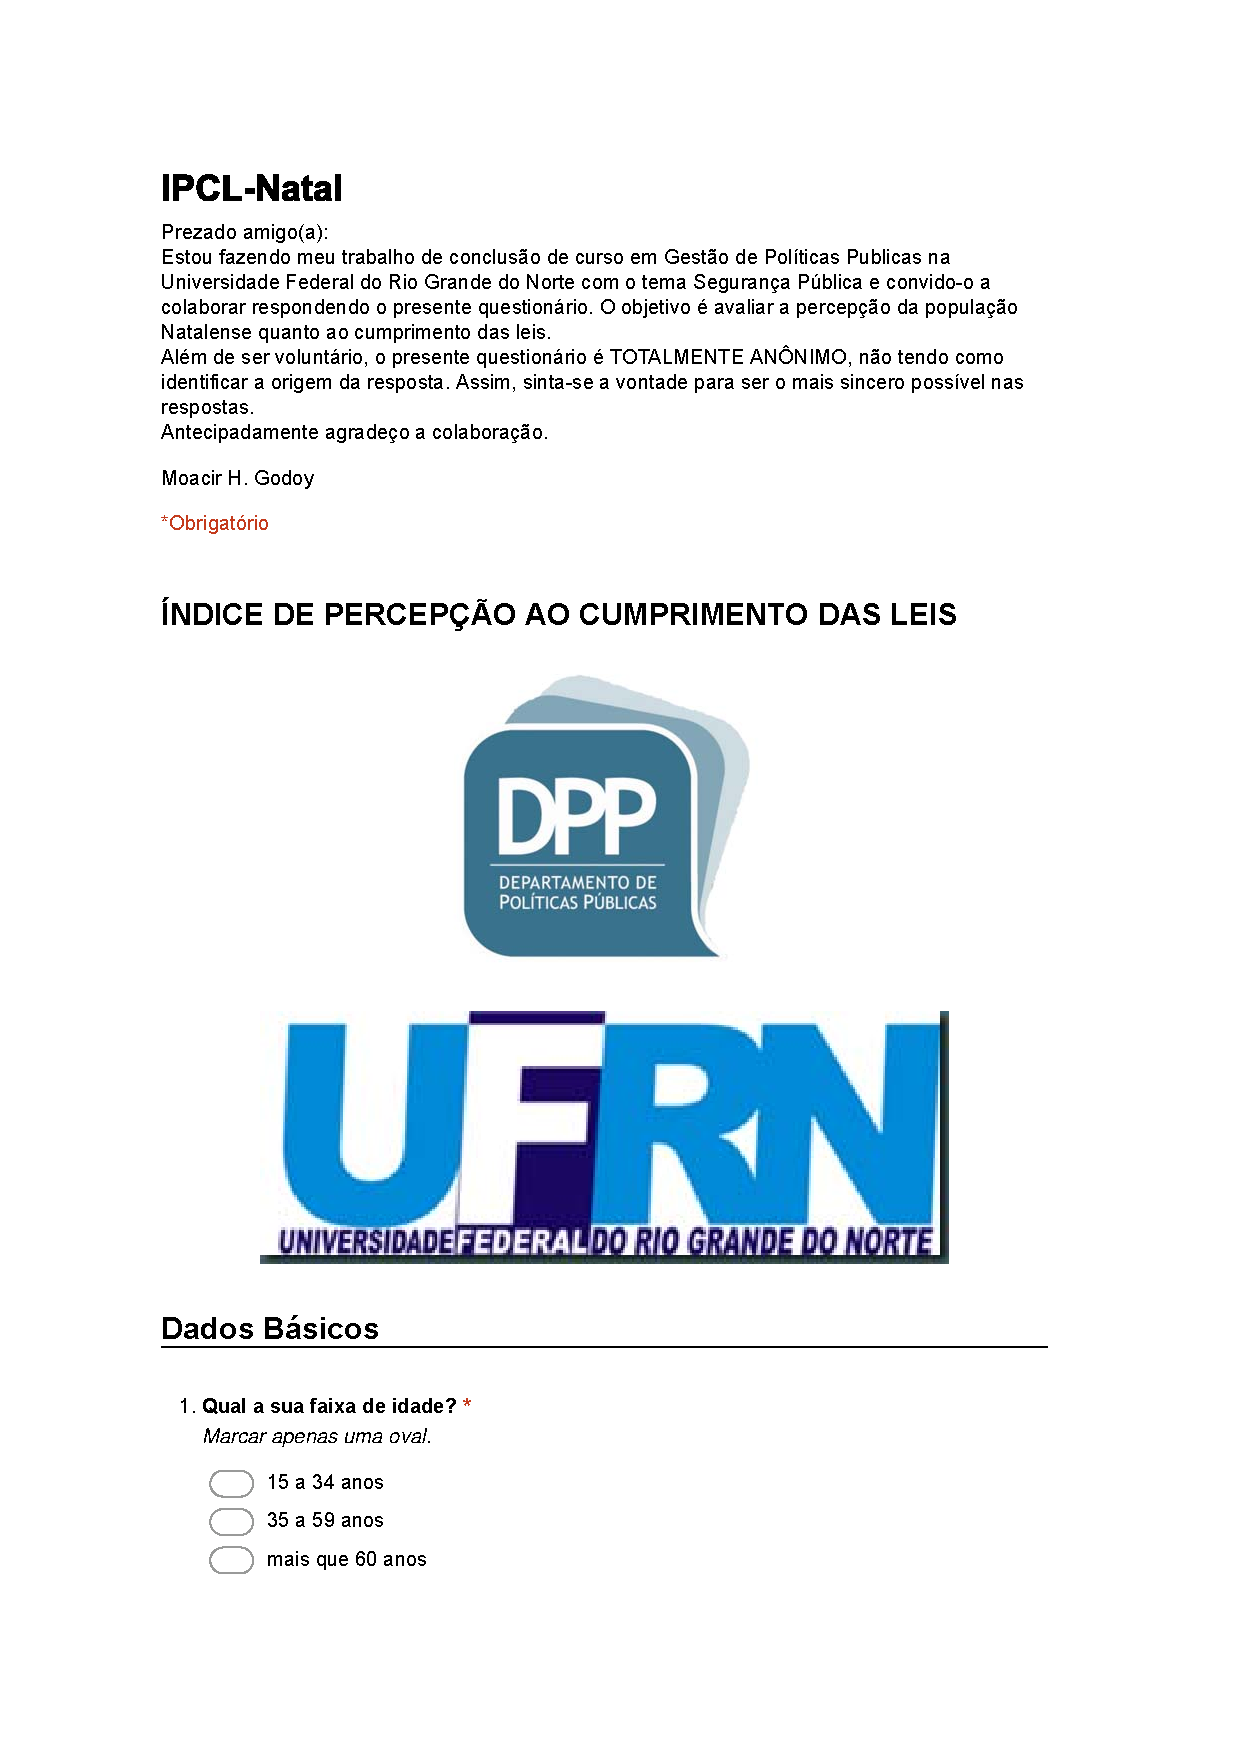
\includepdf[pages=-]{IPCL-Natal-questionario.pdf}
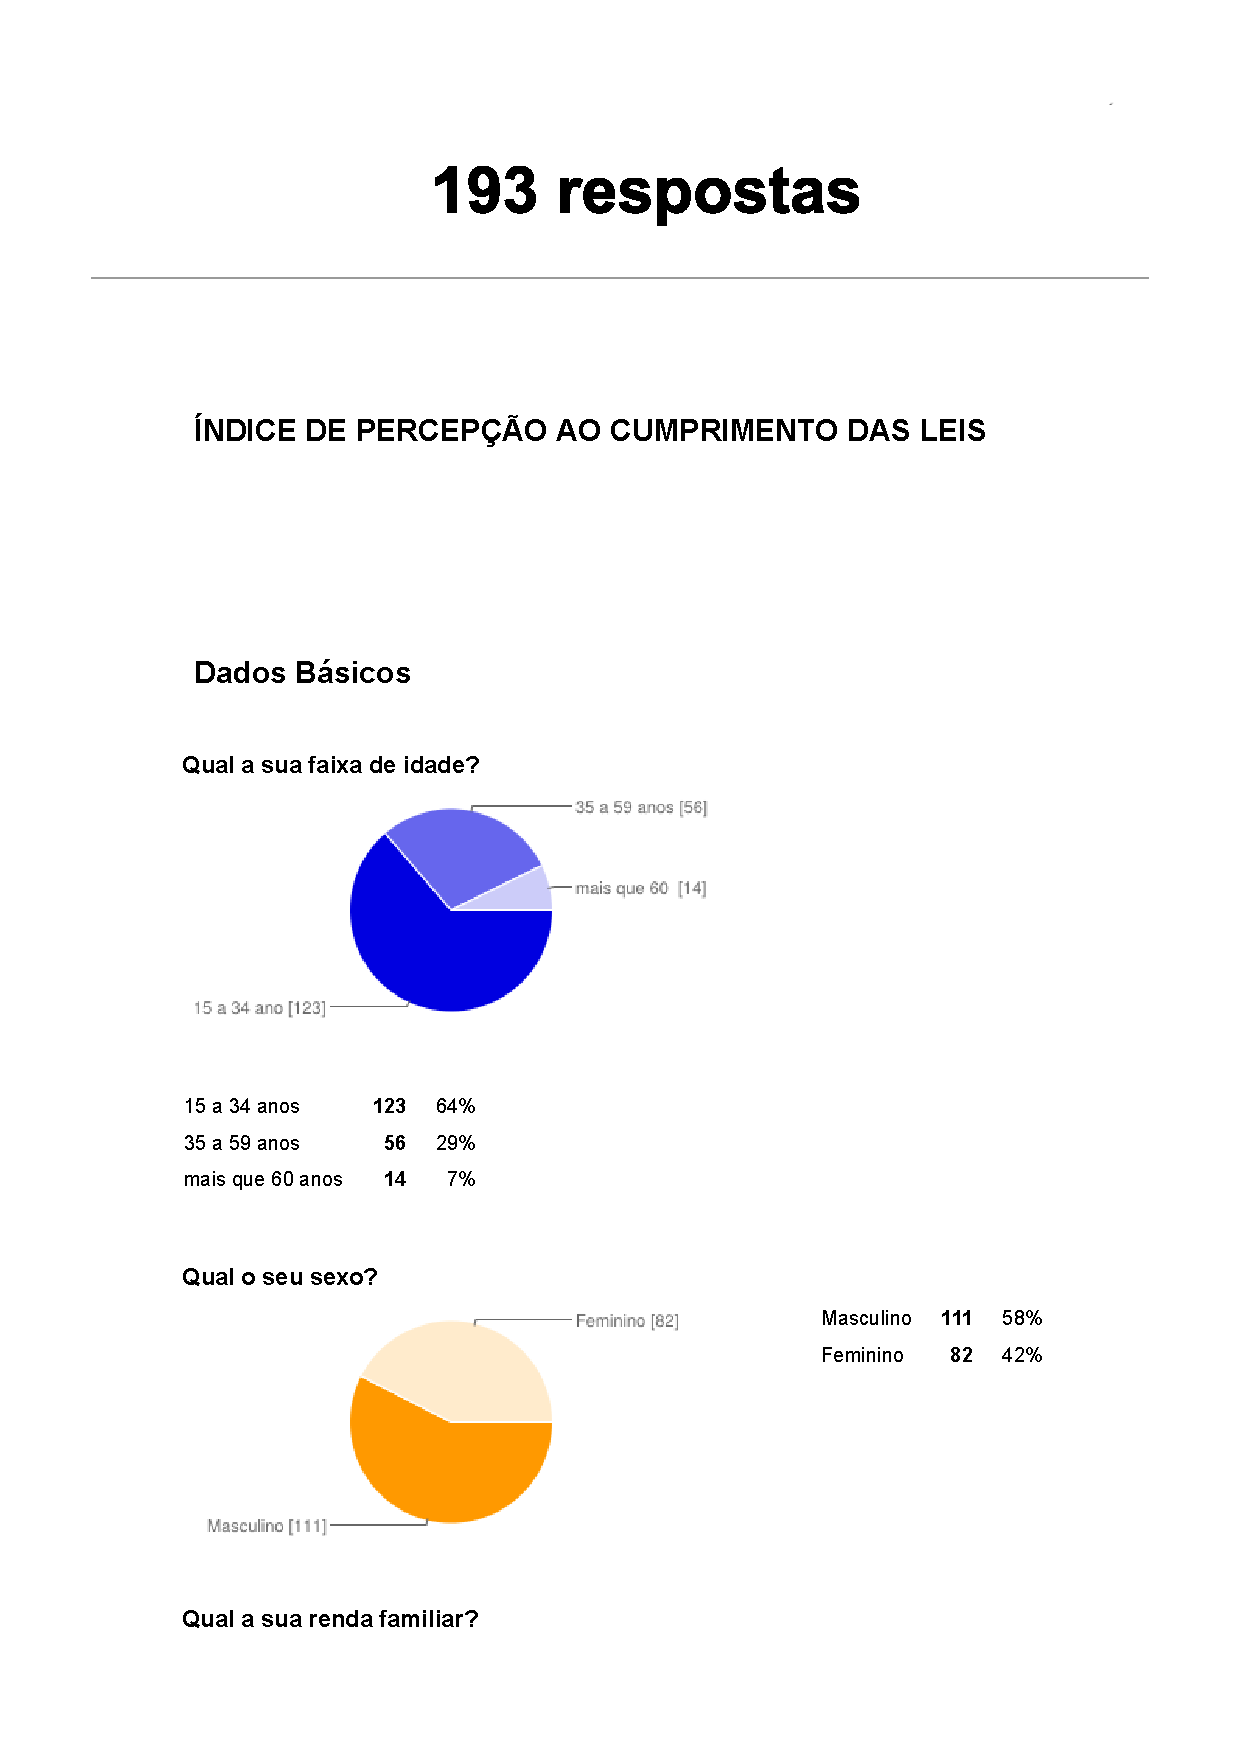
\includepdf[pages=-]{IPCL-Natal-respostas.pdf}

\chapter{Entrevista com o Capitão Styvenson Valentim}
\begin{foto}[!htpb]
	\caption{\label{FotoS}Entrevista com o Cap. Styvenson Valentim - 9 de setembro de 2015}
	\begin{center}
		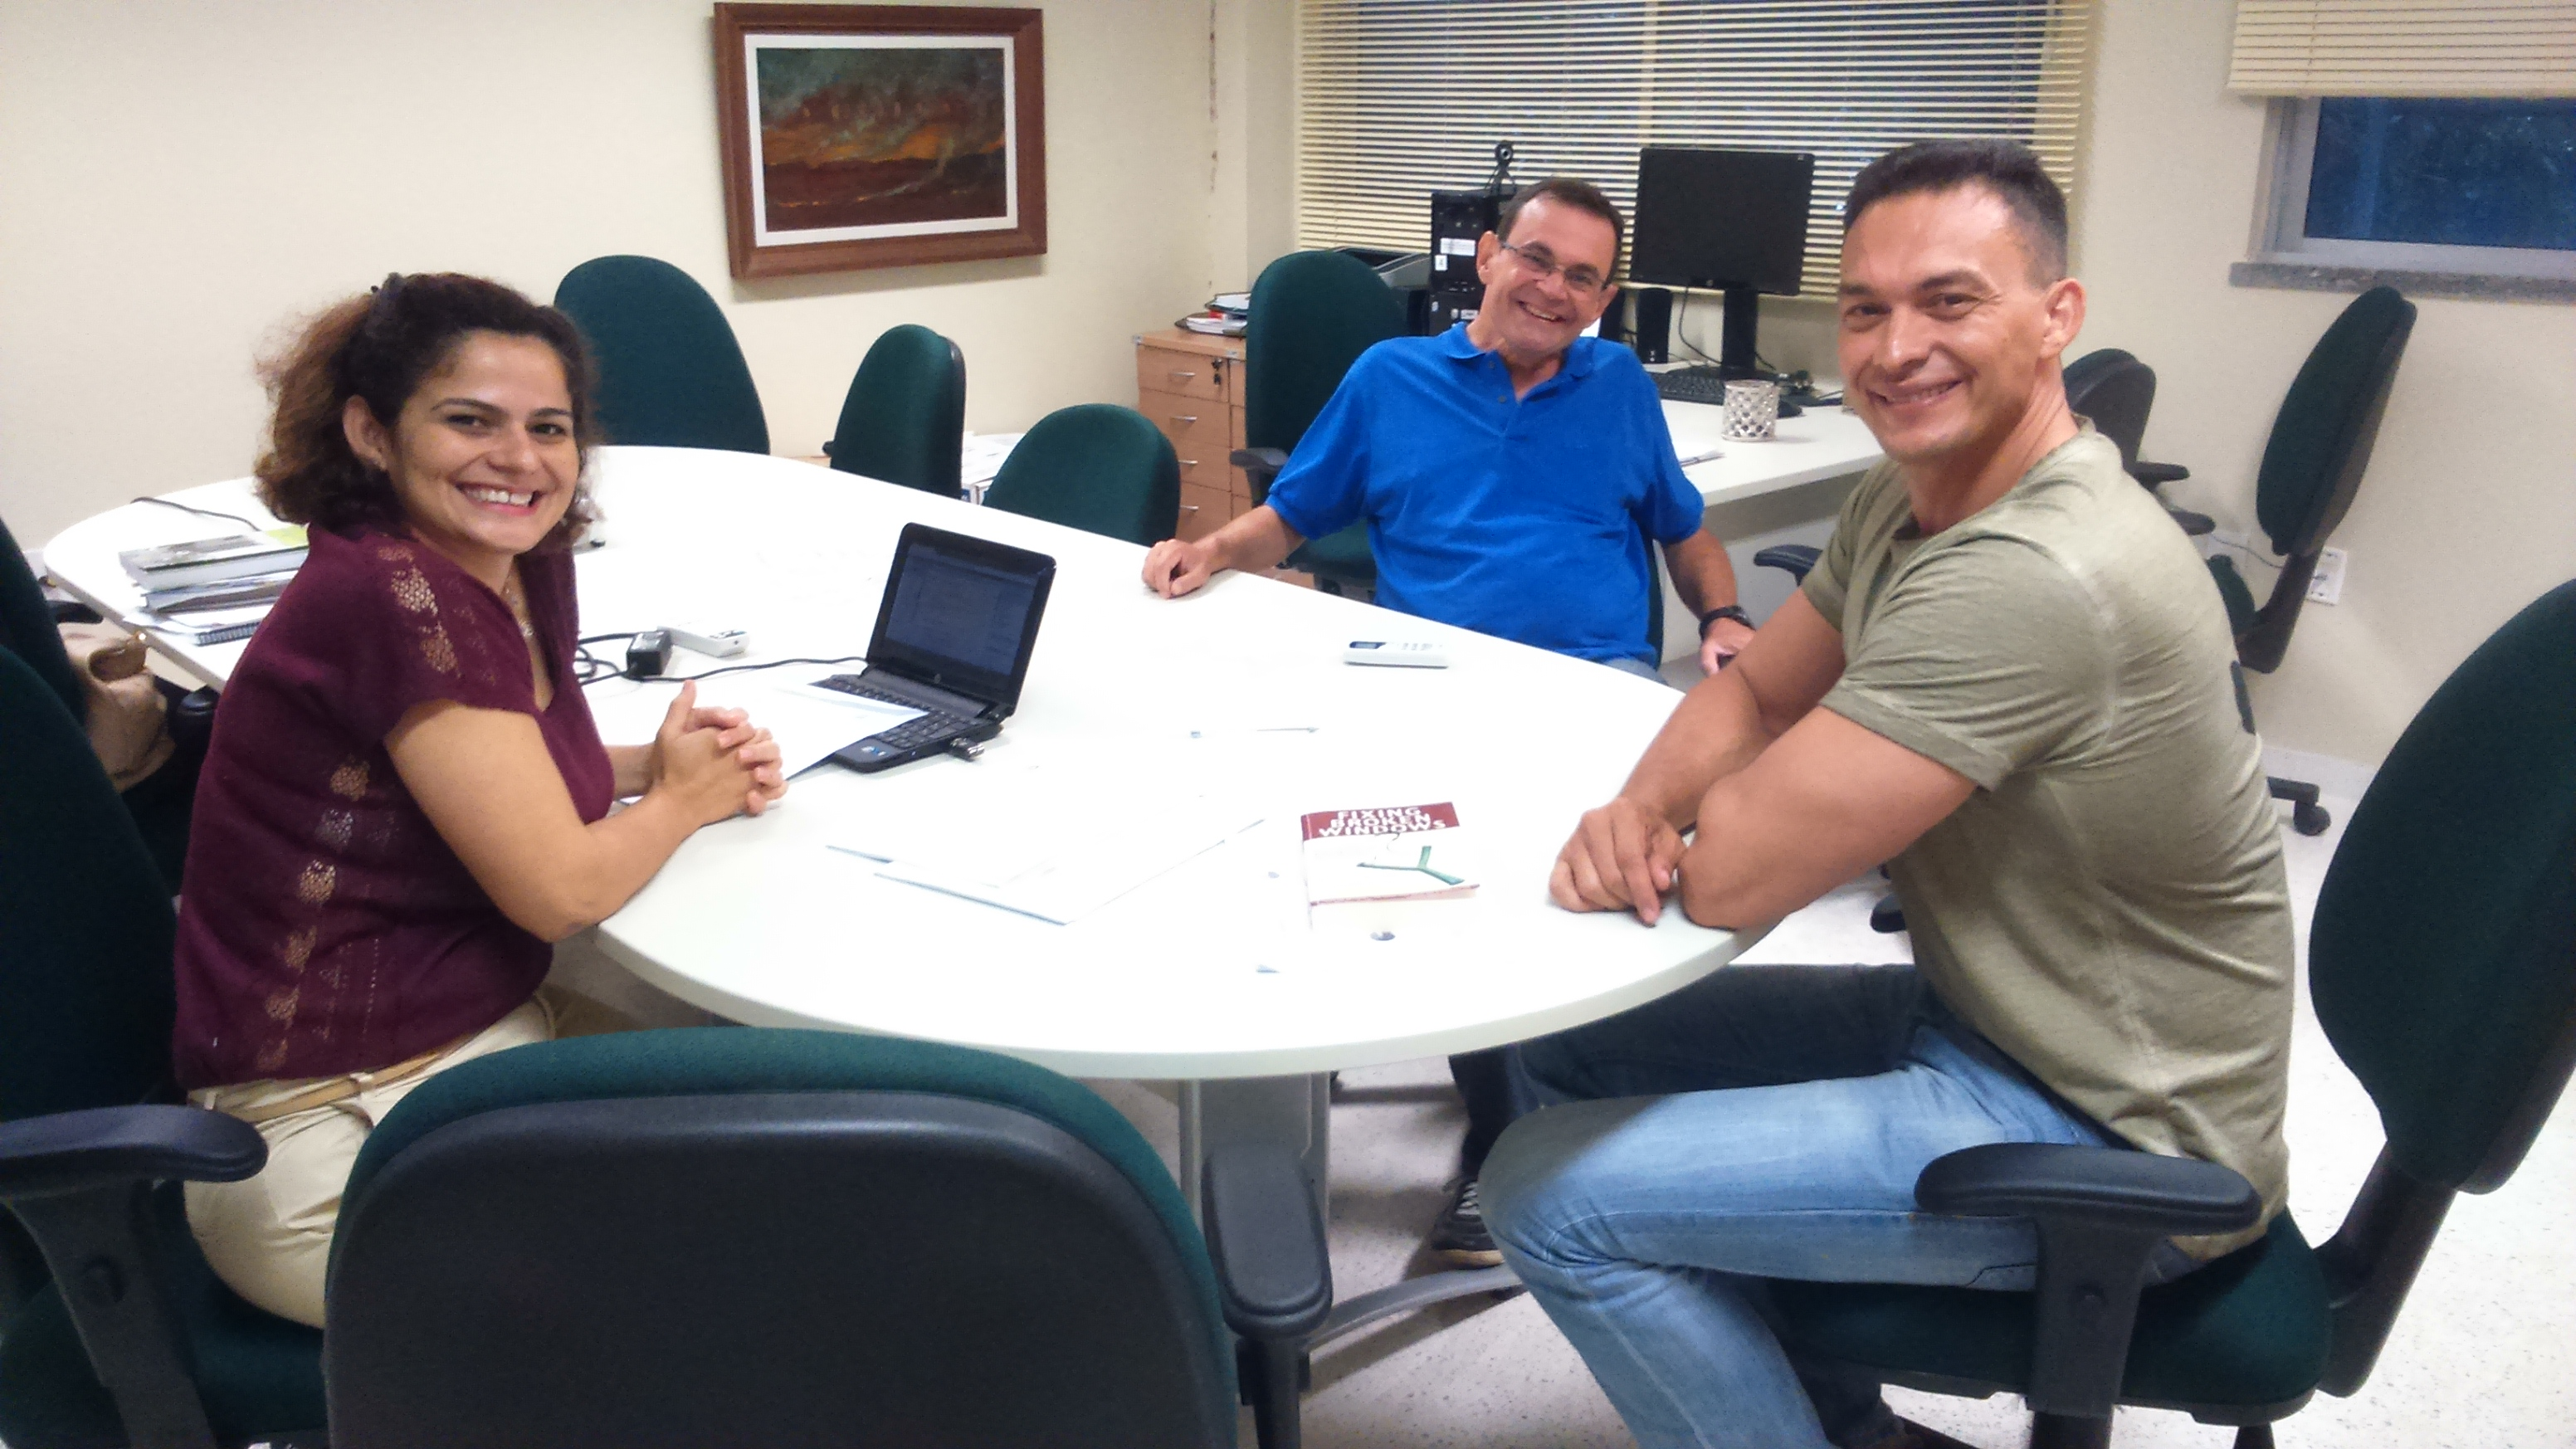
\includegraphics[scale=0.14]{entrevista.jpg}
	\end{center}
	\ABNTEXchapterfont\small{fonte: próprio autor - da esquerda para direita: Profa. Dra. Zoraide Souza Pessoa, Moacir Hardt Godoy, Cap. Styvenson Valentim}
\end{foto}
No dia 9 de setembro de 2015, no prédio do Departamento de Políticas Públicas da Universidade Federal do Rio Grande do Norte, o Capitão da Polícia Militar do Estado do Rio Grande do Norte Styvenson Valentim concedeu um depoimento de quase três horas sobre suas atividades no comando da Operação Lei Seca no Estado. Aos entrevistadores não coube a missão de fazer perguntas, apenas sugerir um encaminhamento, pois transformou-se em um livre pensar da parte do Capitão, com um precioso relato abrangendo vários assuntos relacionados ao tema. A seguir os principais pontos abordados:\\
\hypertarget{B1}{}
\par
\textbf{B1. Sobre a operação lei seca:}\\
	O resultado é um motor que não para. É um motor que está sempre dando resultado(que tem) muita coisa contra, muita coisa desfavorável. Eu acho que durante e até atingir o resultado, tem muita coisa desestimulante, eu não vou mentir a instituição persegue? Demais. Os oficiais querem a cabeça rolando? Querem demais. O próprio órgão que eu estou servindo, às vezes.
	É semelhante a um remédio para um doente. Ah eu estou doente. Quer ficar bom tem que tomar remédio, mas é ruim, vai fazer mal, as vezes quase não engole, mas tem que aceitar porque o resultado todinho como eu disse hoje de manhã (em uma palestra) é querendo ou não que eu perceba que deveria ser um estudo do setor de ciências sociais, é a mudança de comportamento tão rápida em menos de um, dois anos, muita gente 14, 15, 20\% já está começando a assumir que não pratica mais. O simples fato, uma coisa tão pequena, o código de trânsito não tem a mesma plenitude do Código Penal . O CP é um código altamente pesado, porque nós brasileiros só entendemos que é punição só se for realmente na prisão, tirar a liberdade da pessoa, chegar a esse nível, querendo ou não o brasileiro está satisfeito com a punição, porque ele está preso. A ideia que a gente tem hoje com a lei 12760/2012 que é a atual, a que tirou os limites, zerou a capacidade… e por que o Estado fez isso? Porque gerou uma dúvida de quanto eu posso, quanto eu  devo,  virou uma bagunça na questão da defesa, a lei ficou ineficiente e ineficaz, porque se eu tomo um copinho desse não sei quanto vai dar se estou no permitido, no administrativo ou no criminal, eu me recuso a fazer (o exame) então não teria como se avaliar em qual situação a pessoa estaria já que existe uma permissão. É na mudança da lei que eu fui, porque com a mudança lei, no momento que eu permito e eu recuso pelo direito constitucional de não produzir prova, o que acontece? Eu me recusei, eu não tenho (Cap, Styvenson) , juiz não tem, promotor  nenhum tem, policial nenhum vai ter como dizer em qual nível estava. Eu estava no permitido, no administrativo ou criminal se eu não produzi a prova que seria o exame de dosagem alcoólica? Aí no momento que a lei veio e disse opa! O erro está aqui, na permissão. Zera. Zera essa aqui, tira, só deixa duas agora, administrativa e criminal, escolha em qual vai estar. Justamente para tirar essa dúvida, porque a falha na lei causava o sentimento… porque a população é o seguinte: no momento que ela procura falha na lei e achou aí causa uma sensação de eu vou fazer porque tem falha. Houve a discussão agora em Mossoró, eu levei 18 presos,  o delegado soltou 8, pela produção da contraprova que será a minha tese futura que eu entrei na pós em penal, porque não entra na minha cabeça o que foi feito. Mas naquele momento eu nem discuti, a autoridade é ele, eu tinha até certa autoridade, mas não era o momento de se discutir aquilo ali.  Mas a intenção é no minuto que aconteceu esse fato gerou para outros  a possibilidade. Epa! Se lá foi então eu posso. As pessoas, está vendo como elas procuram algo para transgredir? 
	Vamos lá: o sr. está passando em uma rua aí tem uma casa, cão feroz, demônio solto na casa, o sr. vai pular? Dificilmente. Aconteceu em SP. O cara pulou, o cachorro devorou o rosto dele todinho, o dono teve que pagar uma cirurgia plástica para o cara que entrou na casa. Dificilmente a gente quer correr riscos, se a gente for ver pela teoria dos crimes que o sr. fez, assalto em Natal tem um perfil, como tem o perfil de quem morre mais, perfil de quem causa maior infração de trânsito. Voltar para \hyperlink{W1}{Análise SWOT}\\
	\hypertarget{B2}{}
	\par
	\textbf{B2. Os efeitos:}\\
	No início em 2014 quando começamos a fazer as blitz da lei seca, é incrível como o número de mulheres caiu em menos de um ano. Mulher é mais rápida para aprender?  Aí vem do comportamento, desde a origem… como é que mulher brinca quando é criança? Bonequinha, casamento, filhinho, casinha, cozinha… Como é que a gente brinca? Tiro, polícia e ladrão, carro batendo, destruindo tudo… então por isso que a gente homem é mais resistente, As mulheres num instante aprenderam. Eu recebo depoimentos no facebook , no whats up de mãe dizendo “ei graças a Deus, agora durmo tranquila, meu filho chega em casa, meu marido está em casa, não sai mais de casa. Melhor cair na fiscalização do que lá no ITEP (o IML de Natal), num caixão. Mas é o tratamento de choque. É o caso do fumante: fumou a vida toda, teve um infarto… “não quero morrer não, vou deixar o cigarro” . Porque a dependência química é isso, a dependência do álcool… eu vou dizer, a pesquisa que o sr fez tem muita influencia de tudo isso aí. Não estou falando só do álcool não, de muitos. É muito difícil você pegar um bandido, um criminoso que vá limpo, com a cara limpa fazer alguma coisa.  Ele está tranquilão para fazer as coisas? Nãããão… ele está com muita adrenalina, ele tem que estar com muita dopamina no sangue. \hyperlink{O2}{Voltar para a Análise SWOT} - \hyperlink{beb2}{Voltar para o Gráfico 9}\\
	\hypertarget{B3}{}
	\par
	\textbf{B3. Da educação atual:}\\
	Naturalmente a gente sabe o que é certo e errado. Mas por que veio o arcabouço de tantas leis? Porque em princípio, principalmente em nosso país que há lei para tudo, lei para fila de banco, lei para jogar papel pela janela do carro. Precisava de uma lei para respeitar o idoso? Precisava de uma lei para dizer que uma criança tem que ser tratada de forma adequada?  Eu acho que não precisava, mas parece que a gente se torna, eu digo que quanto mais racionalidade, mais selvagem fica, parece brincadeira, estão invertendo as coisas. Quanto mais estuda, mais ignorante está ficando. É o que eu percebo. Pq se você for analisar … Se eu faço uma blitz na zona sul  é uma destruição, é gente jogando coisa, é bala, é mordida na mão… a gente vai para a zona norte todo mundo aceita tranquilo.  Agora eu pergunto: que espécie de educação é essa? Que lá na zona norte subentende-se, compreendo que são pessoas simples pessoas de baixo poder aquisitivo, pessoas que podem ou não ter mais educação, são as pessoas que mais seguem a regra. Aí você vai para a zona sul você tem um índice altíssimo, não é de apreensão não,  é de alto desrespeito… não é à lei não, é a coisa mais simples que existe na sociedade que é a instituição familiar. O filho, o pai vai pagar, isso eu presenciei, o pai, está indo para a delegacia com o dinheiro na mão, contando de cabeça baixa para ver se tem dinheiro para pagar a fiança, eu ouço um grito de dentro da jaula: “paga essa p* aí véio, pra gente ir tomar outra”. Na minha cabeça veio, logo no momento,  o pai passou a vida toda bebendo com o filho, não tem respeito nenhum, perdeu, acabou. Postura de pai é outra. Eu honestamente não sou pedagogo, minha mulher  é pedagoga, eu rebato todas as teorias de pedagogia atuais de que o professor tem que ser amigo, que o pai tem que ser amigo do filho. Não, meu pai nunca foi meu amigo, meu pai foi meu pai. Meu pai sempre foi meu pai e até hoje respeito ele. Porque se ele fosse meu amigo, eu poderia hoje estar desrespeitando, dando tapinha nas costas, eu não pediria mais a benção, eu tenho 40 anos de idade e ainda peço a benção à minha mãe e meu pai.	Será que a minha educação foi errada ou o que eu vejo por aí é a certa?  Entendeu como está a situação? Hoje a sociedade, porque se eu fosse falar o que eu faço, o que eu vejo, é tanto estudo de psicologia… eu vou dizer, não tem condições, certas pessoas tem que aceitar que hoje  a gente está vivendo um problema seríssimo de saúde não falo mais de crime de transito, de infração de transito, eu falo de saude publica. As pessoas estão num ponto de tanta alienação de achar que diversão é encher a cara para não ver mais nada. O que se tem hoje é só música falando de jovem beber, carrão, depreciando mulher, esculhambando com a mulher e o povo acha o máximo. O pai liga o som de manhã cedo com o menino sentado atrás sem cinto, sem cadeirinha, sem nada e bota logo “garota safada”. Menino de 6-7 anos de idade já começa a cantar sem saber o que está cantando. Mas naquele momento já está formando o caráter dele e nem sabe disso. Porque se o pai senta para assistir um programa e diz vem cá meu filho assistir o Discovery, ele morre.  Ele morre porque nem sabe o que está passando, porque ele estudou e nem sabe o que aprendeu, não aprendeu nada. O filho chega “pai estou com dúvida aqui em alguma coisa” “espera aí que vou chamar um professor particular”  ou “vai pesquisar na internet” . É o que o Sérgio Cortella (filósofo e educador) fala da escolarização, de repassar para a escola uma competência que não é dela. O simples fato (da criança) ter um celular e o outro já não ter causa uma discórdia.  (se vê o pai e a mãe bebendo) Vai pensar “se as pessoas que admiro estão fazendo então eu posso fazer também”. E quando você quiser puxar o freio vai acontecer o que? “paga essa p* aí véio que eu quero ir embora tomar uma”. Está vendo agora? A associação? Bom é escola militar. Aí seria a solução para todos os problemas. Não é por eu ser militar não, porque tenho pavor ao militarismo, mas é porque eu vejo o quanto o militarismo regula a vida de uma pessoa. E que se você não quer o tratamento não é o libertino que tem aqui fora. A primeira coisa que aprendi quando entrei no quartel foi “a sua democracia ficou lá fora, aqui dentro é militarismo”. É não senhor, sim senhor e acabou. \hyperlink{W11}{Voltar para Análise SWOT}
	\hypertarget{B4}{}
	\par
	\textbf{B4. Sobre o trabalho na polícia:}\\
	Eu já cheguei num nível de governo que não é bom. Sabe por que não é bom? A sensação que dá é que só um faz, só um funciona, a sensação que a população tem, que as pessoas têm é que só eu quero aparecer eu quero ser melhor e não causa/consequência. Causa: fiz meu trabalho da forma que deveria ser. Consequência: aconteceu.	Por que nem todos chegam no nível de sucesso sobre o que querem fazer? Porque muitos param no meio do caminho. Por que com a febre do FIES, em vez de melhorar o ensino, não muda a qualidade? Porque pegou todo mundo de qualquer jeito, agora se faz apresentação de TCC (Trabalho de Conclusão de Curso) pela internet. Os funcionários públicos são interessantes, (quando) eu estou na blitz pelo menos 50 celulares são apontados para mim, 50 toda noite esperando uma falha, um erro, esperando um grito, esperando um palavrão, um defeito, deslize, criar uma figura que eu não sou, criaram uma figura de perfeição, coisa que eu não sou. Mas hoje o que eu entendo é o seguinte: ele vai errar, ele vai uma hora cansar , uma hora ele vai tomar água. A ideia que se tem é uma ideia quase sobrenatural. Não bebe água, não come, não dorme, está em todo canto, todo lugar, no mesmo momento. Se acontece alguma coisa ali, o trânsito para é dito que eu estou fazendo alguma coisa. Eu estou em casa as vezes recebo um whats app, ele está fazendo blitz, eu digo como se eu estou em casa? Alguém está me vendo, é um sósia meu em algum lugar? Olha o que causou na população.É uma coisa que houve discussão há muito tempo, hoje pararam, o direito de ir e vir; é tanto direito que se realmente todo mundo fizesse e cumprisse o seu dever, eu não estaria fazendo o que estou. Sabe por quê? Quando eu comecei meu trabalho lá na polícia militar; se pegar uma estatística de 2006 quando eu fui para a zona oeste de Natal, Felipe Camarão, segunda companhia do batalhão, a taxa era altíssima e o trabalho que foi feito quando eu comecei lá, reduziu a quase um homicídio por mês, pelo simples fato de estar presente, pelo simples fato de saber que em tal rua ocorria a maior incidência para brigas de traficantes, o simples fato de saber que das 24 h até tantas horas o bar em frente a rodoviária causava esse tipo de incidência, faz uma abordagem 2 a 3 vezes por noite, chega ali e aborda aquele pessoal para eles terem a certeza que a gente está ali, não é a sensação não, porque a polícia uma palavra que me dá um pouco de angústia, sensação de segurança. Se está frio, eu tenho que sentir frio e não a sensação de frio. Eu tenho que ter a certeza que eu estou ali. O que acontece hoje nas “blitz”? Eu transferi tudo isso para a polícia de trânsito. Não vou mentir que eu não dou brecha, que eu não dou falhas, se eu vou fazer uma blitz numa via eu torno aquela via de uma forma que não tem como fugir. Não adianta parar o carro, não adianta trocar de motorista. A certeza que eu vou lhe dar é que você vai ser preso e punido. Só lhe dou uma certeza que é esta. Então isso gerou o terror e as pessoas aprenderam através do medo. Não adianta (querer) pagar, não adianta (querer) subornar, não adianta dizer que é fulano, que a punição vai ser a mesma. Entendeu a que nível chegou? Essa sensação, quando o ser humano comum vê outro sendo autuado e algemado, ele pensa “deixe eu ficar quieto aqui na minha, que se fulano de tal tem esse poder todinho, a sociedade está tendo um tratamento desse nível, eu que não tenho nada, só um telefone e um telefone de alguém, então eu não vou nem tentar”. A sensação foi essa, demorou.
	\hypertarget{B5}{}
	\par
	\textbf{B5. A pressão das “vítimas”:} \\
	Faço meu trabalho, estou sendo perseguido hoje, eu tenho direito a errar? Não, dificilmente. Estou na mão de quem? De uma matilha que está louca para te devorar porque foi criado aquele estereótipo que eu não criei, que eu não sou. Foram atrás de um carro meu atrasado. Entraram no sistema do DETRAN, procuraram carro atrasado, cheque, cartão de crédito, se eu devia, se eu tinha ficha corrida, revistaram minha vida todinha para tornar pública. Aconteceu isso com o Sérgio Moro, o PT revirou a vida dele todinha, para atingir a vida pessoal da pessoa. Acharam um ano atrasado de DPVAT, de 1999, 60 reais, eu paguei. Mas quem fez aquilo para mim me fez um bem danado. Ele nem imagina o bem que me fez porque agora estou com as antenas todas alertadas.	Quem me fiscaliza? Eu tenho os olhos de toda a sociedade em mim. Isso gerou uma superexposição de um direito que eu não posso reclamar,  que é a minha privacidade, da minha liberdade. Eu não tenho mais como reclamar, mas tudo isso por um trabalho só.\hyperlink{Sty1}{Voltar para o texto}
	\hypertarget{B6}{}
	\par
	\textbf{B6. Para implantar uma política de tolerância zero :} \\
	Primeiro (é preciso) ter coragem. Nem todo mundo tem a coragem de chegar e tirar tudo ou reduzir naquele momento uma situação que vai tirar o direito de uma pessoa em detrimento de uma coisa bem maior que é a segurança coletiva. Se for analisar, o direito não foi feito para um, o direito foi feito para a coletividade. Não existe direito particular. Por que nas blitz que eu faço  de 1000 ficam 50-60? Afinal o direito não é para todos? E só 60 ficaram? São 60 pessoas que estão dentro daquela previsão? Dentro daquele contexto (da tolerância zero)? O que falta dentro desse contexto, não é dar uma viatura nova, uma arma potente, fazer concurso, porque é nível superior.  Não confunda grau de instrução com qualidade, porque o sonho de todo mundo que está aí fora é entrar para o serviço público (estabilidade) para mim é preguiça. Eu venho de uma instituição em que você tem 5 pessoas para atender alguém, eles ficam papeando, tomando café quando tem gente para ser atendida. Ficam contando da vida, como está seu filho e quando faltam 5 minutos para a hora do almoço, eles falam que quando voltarmos atendemos. Quando volta a tarde, só tem 2 que na verdade deveriam ser 5, eu vejo isso todo dia, agora o que precisa é fiscalização, para justamente o serviço público funcionar. Agora, uma fiscalização eficiente.\hyperlink{T0}{Voltar para Conclusões}
	\hypertarget{B7}{}
	\par
	\textbf{B7. Metodologia da abordagem} \\
	Se você me der papel e lápis eu vou mostrar como montei uma \textit{blitz}, eu montei de uma forma matemática, onde o próprio policial fiscaliza o outro. Então eu fiz uma fiscalização que não tem como quebrar o negócio e eu fico a 1 km de distância, com o rádio. Antigamente as blitz se você for ver, favorece ao sorteio, você fica, você passa. No minuto que eu disse “não passa nada, fica todo mundo aí” causou um medo maior ainda. Lembra que eu disse da carteirada, da cantada feminina (momentos antes da gravação) se for a Giselle B\"{u}ndchen não vai passar, fica todo mundo, são feitos 1000 testes por blitz, 2000 dependendo do evento, não sai enquanto não tiver passado todo mundo. Eu já fiz teste em que, quando o último passou, a gente prendeu. Vou mostrar na prática como é que funciona: Isso aqui é uma ruazinha. Faço uma matriz, matriz matemática, linha/coluna. Policial 1,1 – 1,2… O carro entra aqui para ser abordado. No início foi difícil, eu tive que quebrar a cabeça. Policial linha 1 coluna 1, Policial linha 2, coluna 1 (mostra no desenho - fig. 3).
		\begin{figure}[!htpb]%NBR 14724:2011 item 5.8
		\caption{Esquema das \textit{blitz} da lei seca}
		\begin{center}
		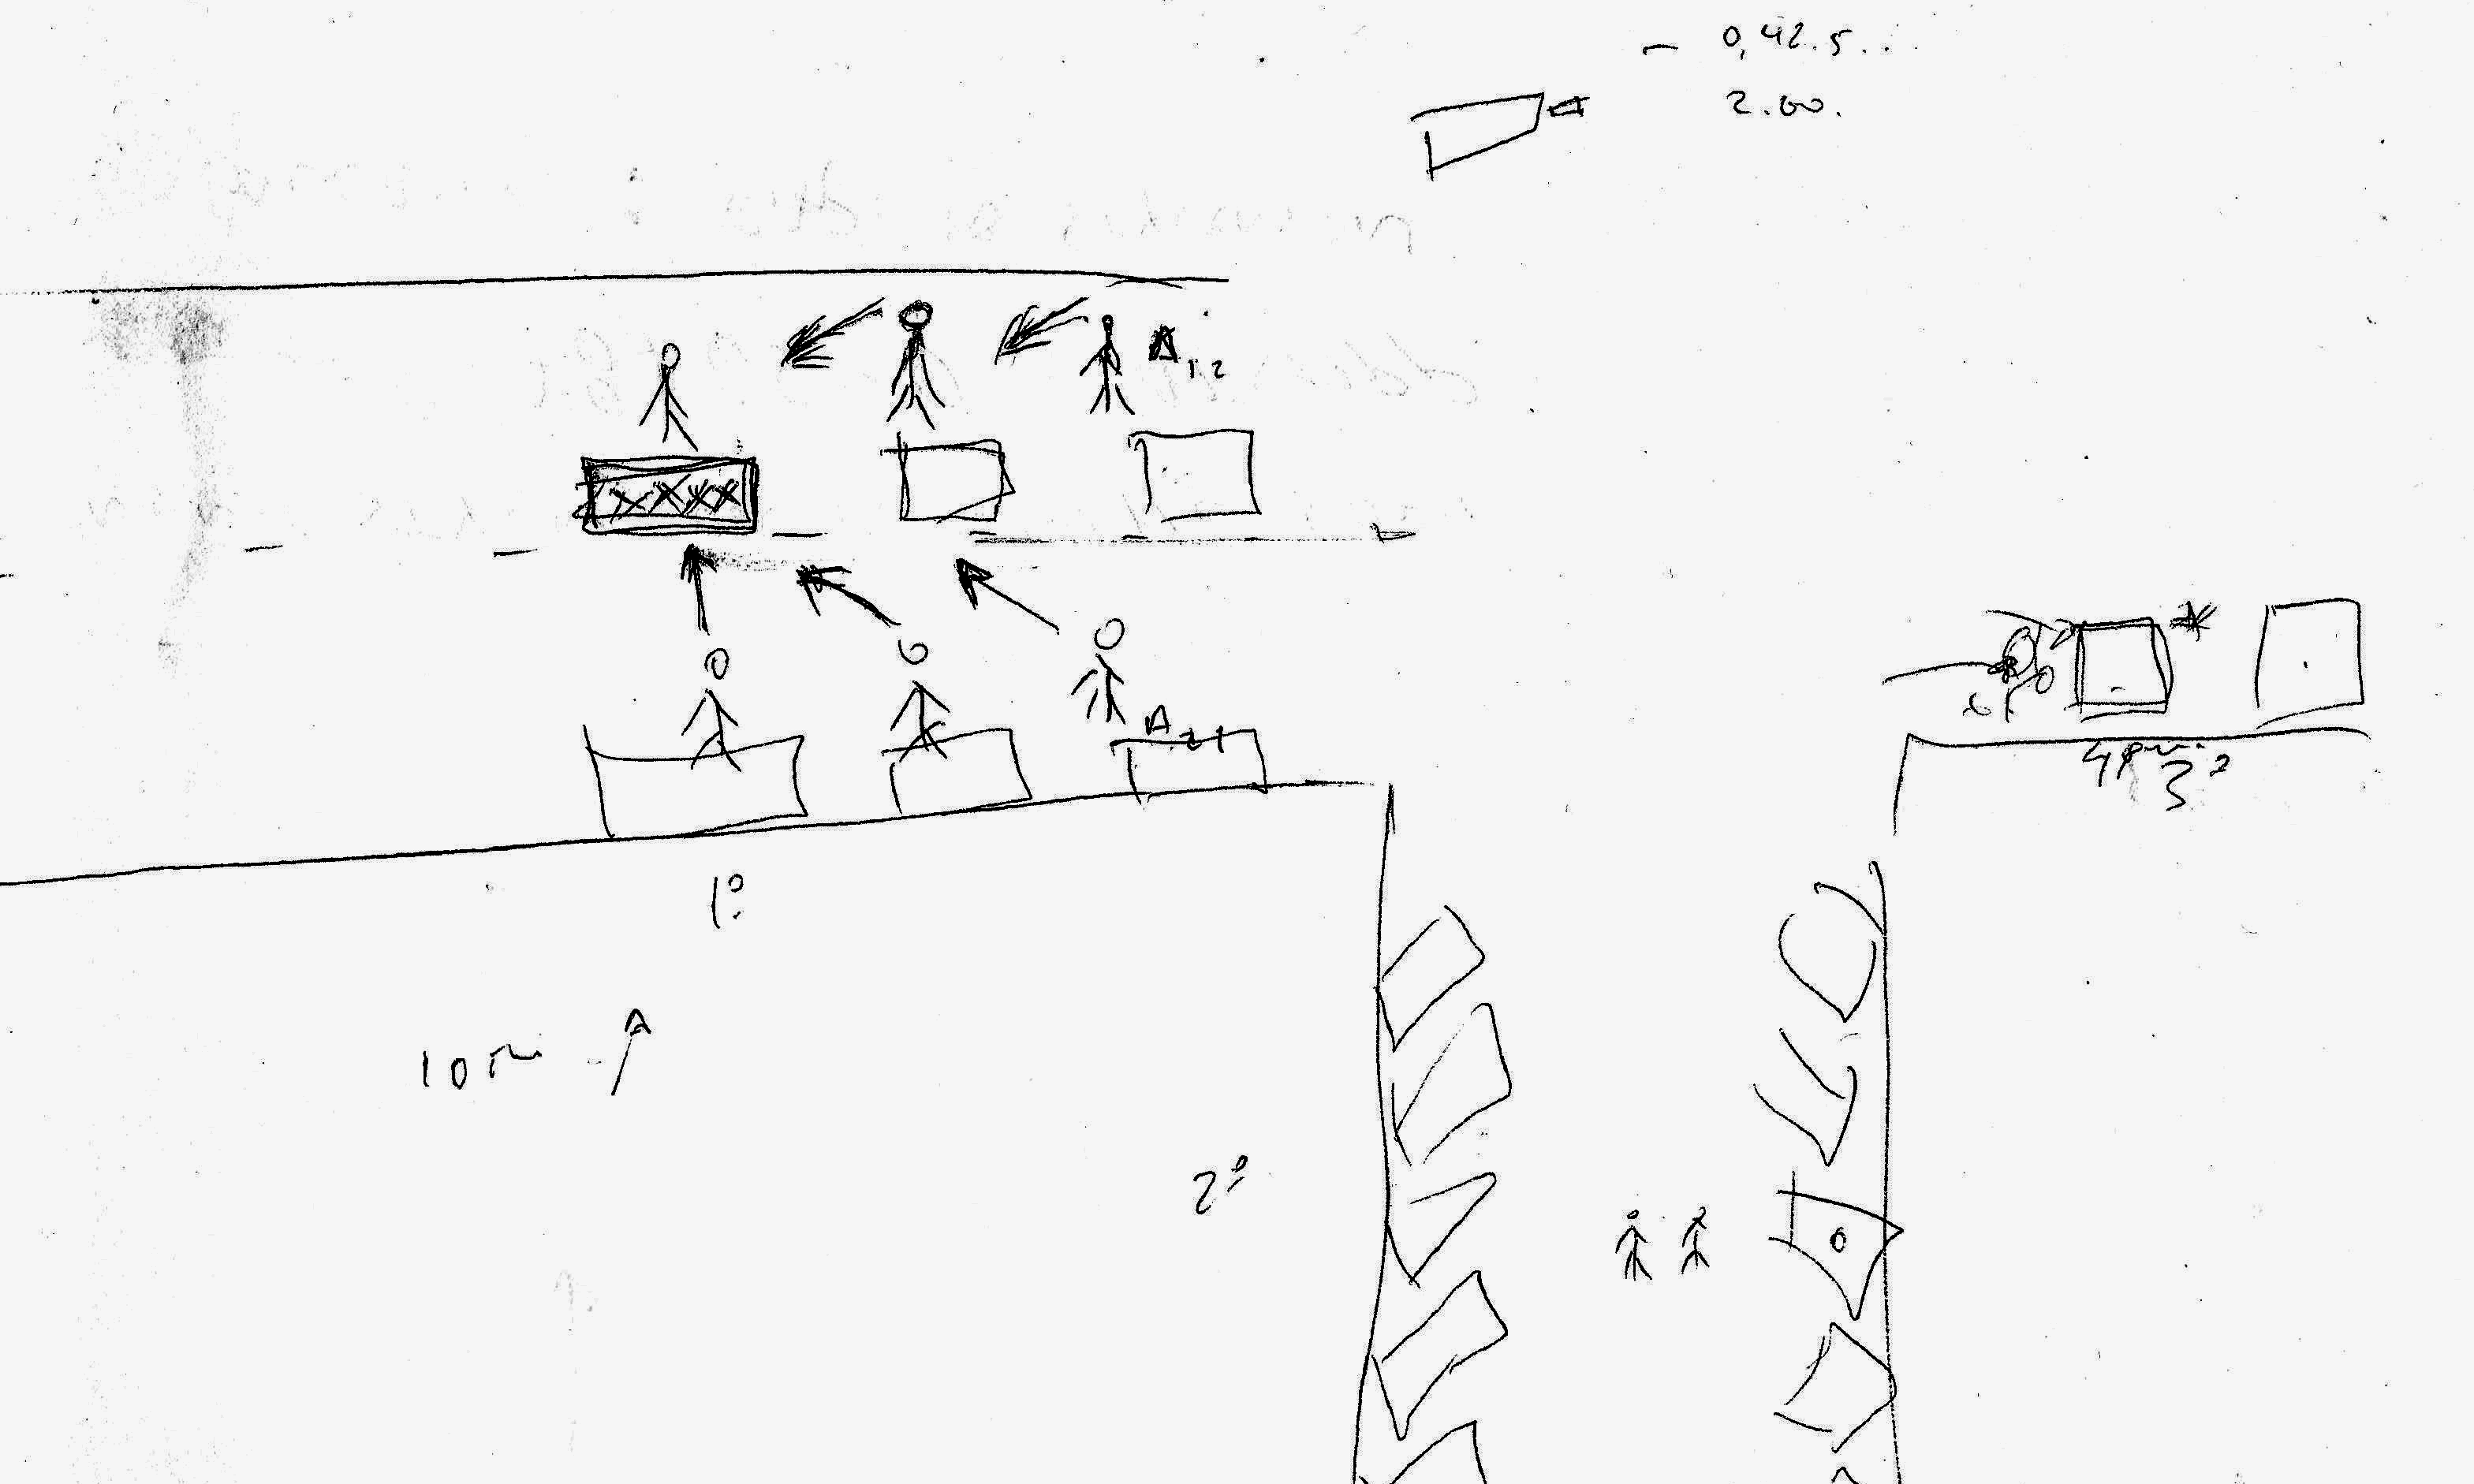
\includegraphics[scale=0.2]{blitz1}
		\end{center}
		\ABNTEXchapterfont\small{fonte:Capitão Styvenson Valentim - 9.9.2015}
		\label{blitz}
	\end{figure}  
	Esse policial ele não faz a coisa que ele quer não. Eu sei que um exame de etilômetro, eu sei porque eu fiz, eu fiz o teste dando zero e fiz o teste dando alguma coisa. O teste dando zero ele leva de zero até 42 segundos para ser realizado, ele dando alguma coisa, pode chegar até 2 minutos. Então eu sabia que de zero a 2 minutos era o tempo de abordagem para cada policial desse. Então a cada 2 minutos os meus 6 policiais tinham que fazer a abordagem completa. “Boa noite, polícia da lei seca, o sr. pode fazer o teste do etilômetro?”. Então eu estipulei 3 minutos como o teste, a cada 3 minutos, 6 carros serão abordados. Ah só isso, onde está o grande mistério? Não,  vamos dizer que esse fulano aqui, (faz o hachurado na posição 1,1), esse fulano aqui está com má intenção, está negociando; ou esse cara que está conduzindo o carro é uma autoridade, está dando uma “carteirada”, está dando problema. Passaram os 3 minutos todos os carros saíram da via, só ficou esse, o relógio quebrou. Porque travou tudo. (aponta para os outros policiais no desenho) Esse vai olhar para esse, vai olhar pra esse… todos (os demais policiais) vão olhar para ele esperando ele liberar esse carro para entrarem 6 de novo. Os carros não entram aleatório não, entram de 6 em 6. Só entram 6 (novos) quando o último passar. Então quando esse não passa por algum motivo que eu não sei qual é, não sei se ele está se favorecendo, se alguém está dificultando, os outros (policiais) começam “ei o que está acontecendo aí, qual o problema?”. Aconteceu que quando um não funciona, os outros querem que funcione porque querem continuar e quando um para todos param. Então todos vão olhar pra esse o que está acontecendo, então esse fica intimidado de querer se corromper. É muito dinheiro mas não dá certo não. Aí pergunta onde é que eu fico aqui? Em canto nenhum. Ainda tem outro grande lance que eu trabalhei por setores. Primeiro setor (abordagem), segundo setor estacionamento. Todos os carros que são apreendidos vem para um ponto. Esses carros já foram abordados, já tiveram a CNH recolhida e o documento apreendido. Então vem para o estacionamento e fica aguardando (setor 2). Setor 3 seria a autuação, crime e administrativo.  Os 3 setores funcionam de forma semelhante. Ficam 3 policiais aqui, justamente para pegar a chave do veículo, revistar o carro, nunca sozinho, ele vai por etapas, o dono do carro acompanhando. No terceiro nível ficam todas as pessoas que vão ser autuadas. Ali ficam mais 4 policiais, fazendo uma ordem por horário de abordagem. E onde eu fico? Nem aqui (setor 1), nem aqui (setor 2), nem aqui (setor 3)., eu fico aqui (aponta para um local fora da blitz), sentado em um banco ouvindo o rádio. Porque eu montei um esquema que não tem como acontecer mais nada porque aqui o povo está fiscalizando (setor 3). Alguém diz “eu sou coronel da polícia”. 60 pessoas se viram e dizem “e daí? O que é que tem você ser coronel da polícia? Aqui você é igual a nós”. E aí começa a discussão. Então as próprias pessoas se resolvem. Entendeu como funciona o sistema? Aqui não acontece nada (setor 2) porque o sujeito já desceu e o policial já tem discurso. É tudo discurso. Discursos 1, 2 e 3. Discurso 1: nunca diga que está preso, nunca dê a voz de prisão naquele momento. A voz de prisão é dada quando ele para o carro (setor 2) porque aqui (setor 1) ele foge. Aqui (setor 3) vai dar tudo certo. Chame sua família, chame alguém. Nunca estressar com o bêbado, poque ele já está estressado. Então a polícia no bem atender é melhor para a gente e para a pessoa abordada, porque eu não vou provocar o que já está provocado. Se eu for irritar alguém que já está irritado vai ser um caos. Eu montei um esquema que não tem como furar. Um policial que saiu, ele liberou um major. Sabe quem denunciou ele? Os outros. Eu não precisei nem me indispor. Os outros policiais disseram “não era para ter feito isso não”. Vai dizer para o Capitão agora. Aí eu disse “preciso dizer o que vai acontecer?”. “É melhor eu sair né?”. “Se você não sair vai levar punição”. Eu cheguei a um ponto que eu não preciso dizer o que fazer mais, porque já virou mecânico.\hyperlink{W2}{Voltar para Análise SWOT}
	\hypertarget{B8}{}
	\par
\textbf{B8. Polícia comunitária:} \\
	O senso de polícia comunitária se não fizer um policiamento adequado ele corrompe no fato: “bom dia dona XXX !! A sra. é dona do mercadinho!! Olha eu sou do policiamento aqui viu? Se precisar de alguma coisa é só chamar a gente”. Aí chega no final da noite, ele vai estar na porta do estabelecimento esperando os 20 reais . Isso é polícia comunitária? Ou acha que isso não acontece? Ou acha que me dar um bolo, um café; a polícia militar é corrompida, eu não tenho que ficar visitando sua casa, almoçar com você. Não, ele só precisa prestar serviço, só isso, é tanta teoria que existe e ninguém faz o que é para fazer. Preste o seu serviço, eu presto o meu e no final dá tudo certo. Por que tem que agradar o policial? Para ele ficar na porta do meu comércio para eu não ser assaltado?  Se for atrás de chamar qualquer viatura, é praxe, é prática, ou nunca viu viatura parada na porta da padaria? Nunca teve curiosidade de saber por quê?
	\hyperlink{PC}{Voltar ao texto}
	\hypertarget{B9}{}
	\par
	\textbf{B9. Sabatina nos subordinados:} \\
	Por que eu sou tão chato com os meus policiais? Por que eu faço prova oral? Como você agiria em situação tal? Porque toda hora eu estou colocando situações pelas quais eles não passaram ainda? Por que toda hora eu estou criando problemas para serem resolvidos?  Para não serem pegos pelo fator surpresa. Por exemplo, isso que eu passo a eles: eu estou aqui fumando a minha maconha, vi a blitz, joguei fora. E aí, prendo, autuo, faço o quê? A cabeça fica (ininteligível, provavelmente sem saber o que fazer). Você não tem tempo para pensar, precisa de uma resposta. Era para ter pensado antes. O problema, resolva em casa, traga a solução, vamos discutir. Eu aqui não tenho tempo para tomar decisões inesperadas. Eu tenho que prever coisas que não aconteceram ainda.. Eu tenho que prever situações para as quais o policial não está preparado. Porque ele só está preparado para ficar na porta da Gosto de Pão (uma padaria em Natal). O que falta é compromisso, o que falta é executar, o que falta é o policial ter uma formação adequada.
	\hypertarget{B10}{}
	\par
	\textbf{B10. Resultados:}\\
	10 policiais, 2 viaturas, 1 van e 20 etilômetros. É isso o que eu tenho. 50.000 abordagens, 7000 CNH apreendidas, 1200 pessoas presas. Nos hospitais, redução do número de acidentes. É muito dinheiro que entra, as blitz estão dando muito mais dinheiro que os emplacamentos, por isso é que sou tratado a pão de ló. Como é que 10 (policiais), 2 viaturas e 20 etilômetros dá um número altíssimo de arrecadação? Querendo ou não, se não errasse não teria, então não há indústria de multas, porque se você ão erra, não tem multa. Errou, vai ser multado. E a melhor conta que eu acho é você não ter gente nos hospitais, não ter famílias perdendo familiares, é não ter pai chorando por filho morto. Essa é a melhor conta que eu acho. Essa é a ponta que me interessa. Porque eu trabalho nessa ponta aqui (a fiscalização) mas a que me interessa é essa aqui (redução de acidentes). Isso aqui não me interessa, quantas CNH eu apreendo, não queria nenhuma, mas infelizmente está acontecendo. É consequência disso, mas a ponta que a gente idealiza é essa (redução de acidentes). Está vendo o que é efetividade com pouca coisa? Aí vai ver o que é impessoalidade quando não tem corporativismo.   Está vendo o que é moralidade? São tantos princípios… \hyperlink{Nat}{Voltar ao texto}
	\hypertarget{B11}{}
	\par
	\textbf{B11. Pressão:}\\
	Só para sentir a pressão. Eu não posso mais ir para um bar, eu não posso ir para restaurante, eu não posso ir para festas. E por que eu não posso? Vou lhe dizer: em blitz tiram pelo menos 30 fotos, param o carro e pedem para tirar foto, alguém filma, alguém pede para fazer vídeo, “manda um abraço para minha mãe”. Chegou a esse nível. Eu estou no supermercado, de cabeça baixa, fazendo compras, alguém tira foto e coloca nas redes sociais. Eu vou para o aeroporto viajar alguém tira foto, vamos beber que ele está viajando. Se eu vou para um aniversário, o garçom me dá refrigerante, vão dizer que é uísque.  É toda hora se policiando, é toda hora evitando, é toda hora se restringindo, é toda hora tentando não errar. Até um copo, se for refrigerante, eu não pego, eu afasto. É toda hora assim, eu não tenho paz, a realidade é essa. Eu não pedi para fazer esse trabalho, em momento algum. Em 2014, quando eu fui chamado de novo para fazer isso, porque em 2012 eu levei 15 dias de cadeia porque eu  abordei um major, aí eu também não fui mais e acharam bom, porque também haviam muitas pressões para acabar, culminou com essa prisão de 15 dias, em 2014 quando determinaram que eu voltasse eu disse que não ia fazer, que não havia interesse, que eu já estava fazendo outros trabalhos. E foi feito. Eu, parece mentira, eu não largo o que eu faço não. Eu faço pela responsabilidade que foi dada. Eu faço hoje porque alguém acredita nesse trabalho. Eu só preciso dar resultados, mostrar que dá certo, que dá para ser feito, viu que serve de exemplo? Olha, vocês que acham que não pode, alguém já fez. Por que você não pode fazer? Você é igual a todo mundo, você tem 2 braços, 2 pernas, agora você tem vontade de querer fazer e responsabilidade.
	\hypertarget{B12}{}
	\par
	\textbf{B12. Solidariedade:} \\
	Eu tenho uma característica que as vezes eu nem quero ter: eu gosto de ajudar as pessoas. Eu me sinto mal de ver alguém precisando e não fazer nada por ela. Poucas pessoas tem conhecimento que eu dou palestras de graça para empresas privadas só em troca de donativos para quem está precisando. Eu não peço nada para mim, poderia pedir. Eu podia trabalhar em polícia comunitária. Não poderia? Mas porque eu não faço? Porque primeiro tem uma legislação que me proíbe. Eu sou dedicação exclusiva, o meu serviço policial, mas também não tem nada que me proíba as palestras, porque é um trabalho extra, eu não estou indo a serviço. É o conhecimento que eu tenho da legislação de trânsito. E o obrigado de suma senhora de 80 anos que foi abandonada em um asilo para mim não tem preço. Escutar de uma criança do Durval Paiva, com câncer,  dizer obrigado por ter vindo, para mim não tem preço.
	|hypertarget{B13}{}
	\par
	\textbf{B13. Sociedade fiscalizando o indivíduo:}\\
	O nível que eu queria de sociedade é que existisse uma coação da própria sociedade com o infrator, eu dei até um exemplo uma vez: eu disse ninguém suporta ver alguém agredindo um velhinho, ninguém suporta, mas mata filho. Ninguém suporta ver criança apanhando, ninguém gosta de ver animal sendo judiado. Houve um linchamento por causa de um estupro. Por que crimes mais potenciais que um estupro são suportados e esse não? Está vendo a cabeça do ser humano como é?
	\hyperlink{Sty}{Voltar para o texto}
	\hypertarget{(B14)}{} 
	\par
	\textbf{B14. O jeitinho:}\\
	(sobre o comentário que as pessoas preferem dar o “jeitinho”) O jeitinho é melhor né? Eu sou esperto. Eu estou com 20 reais, vou dar para o guarda que precisa. Uma vez eu estava em um policiamento no 9 batalhão, na zona oeste de Natal onde acontecem a maior parte dos crimes, eu fiz zona norte e zona oeste, numa dada ocorrência, que foi ocasionada por uma briga de vizinhos, causou lesão corporal, faca, aquela confusão toda, aí eu cheguei, o circo montado, aí eu pedi silêncio que eu queria saber o que estava acontecendo,   e alguém gritou tentando me atingir moralmente: “rapaz, não dá atenção a esse passa-fome não”. Passa-fome na ideia deles é como eles classificam os policiais. Ele achava que ia me tirar do sério. Nisso os outros policiais já ficaram ansiosos para ir pegar, prender, bater. Eu disse calma… eu não vi quem foi, quem falou, no meio da multidão, aproveito o anonimato daquela turba todinha, eu disse: “para quem disse que eu passo fome, acertou. Porque eu passo o dia com 1800 calorias porque realmente para ter 10\% de gordura no meu corpo eu passo fome. Diferente dele aí que está falando que deve ter pelo menos 50\% de gordura no corpo”. Aí a população já indicou quem foi. Foi fulano. Aí começou aquele hehehe todinho ele pegou e saiu. É inteligência para não usar uma coisa que os policiais queriam. Para agredir, bater, prender.
	\hypertarget{B15}{}
	\par
	\textbf{B15. Os desafortunados:}\\ 
	(sobre o comentário “não é porque o indivíduo nasceu no lugar errado, na família errada, que isso serve de justificativa para cometer crimes”) Já foi criada socialmente a historinha do coitado, que não teve estudo, não teve oportunidades. Mas como é que eu trabalhei na zona oeste e 4 horas da manha tinha gente que ia para o trabalho? Só via o pessoal passando de bicicleta para ir trabalhar. E por que nem todo mundo dessa comunidade é bandido? Era para ser 100\% bandido, concorda? Pela teoria de que faltou tudo, de que o Estado não está lá, agora eu sempre disse, eu digo e sou honesto, pelo menos em Felipe Camarão eu nunca vi uma praça de esportes, eu nunca vi uma pista de skate, uma nunca vi uma pista de bicicletas como tem aqui em Ponta Negra, eu nunca vi campo de futebol society, creches, escolas legais, shopping… você já viu um shopping em Felipe Camarão? E por que se exige tanto daquelas pessoas? Por que se culpa tanto elas? Elas não tem o mínimo. O esgoto é aberto, a polícia só chega lá para dar tapa na cara do povo… uma vez eu vi isso. Pessoal estava reclamando, botando em facebook, por que não vai pegar bandido? Gente, não vai por essa passagem. Eu já prendi muito bandido... \hypertarget{B15A}{} \\
	Eu disse uma vez na imprensa: botar uma farda, ir lá na zona oeste, invadir a casa de um pobre, de um coitado, botar o pé na porta, revistar a casa toda, dar uns tapas nele, qualquer policial faz. Qualquer. Ele não precisa ter o mínimo de conhecimento de Constituição, de Código Civil, de invasão de domicílio, de Código Penal, ele não precisa ter o mínimo de conhecimento. Ele vai lá e faz. Agora eu quero ver ele entrar, ele arrombar a mesma porta, lá do Alphaville. Ele nem passa. Eu quero ver ele abordar uma Land Rover, eu quero ver ele botar o proprietário da Land Rover com a cara no chão, no asfalto quente, como ele bota o pessoal da (ininteligível, provavelmente algum lugar em Felipe Camarão). Por que hein? Está vendo o porque daquela pergunta por que as coisas não funcionam?
	\hypertarget{B16}{}
	\par
	\textbf{B16. O policial que trabalha comigo:}\\
	Primeiro o policial tem que se limpar. Uma vez eu respondi uma pergunta que fizeram: que tipo de policial que eu pego? Limpo, não é limpo sem desvio de conduta não. Ele vem eu desmonto ele todinho. Tira sua arma, tira sua farda, tira tudo. Seu poder não está aí não, viu amigo? Seu poder está na sua fala, na sua gesticulação, na sua postura, na sua imagem, no seu cabelo, na sua barba, é o conjunto que vai dar a sua autoridade, não a arma e o murro que vai dar na “fuça” de alguém não. Aí não é respeito, é medo. Voltar para a \hyperlink{W13}{Análise SWOT}\\
				

\chapter{Um pequeno passeio}
No dia 13 de setembro de 2015, o autor do presente trabalho fez um pequeno passeio a partir de sua residência nas proximidades da Av. Ayrton Senna no bairro de Neópolis até a Av. Eng. Roberto Freire no bairro de Capim Macio (Mapa 3), com o objetivo de averiguar a presença do “paradigma de Zimbardo” nesse trajeto. Um trecho de apenas 3,4 km, que leva em média 8 minutos para ser percorrido. As fotos abaixo são apenas uma amostra do que foi encontrado. A mesma situação ocorre em todas as ruas e avenidas adjacentes e muito provavelmente em todo o município de Natal.
\newpage
\begin{mapa}[!htpb]
	\caption{\label{Mapa3}Roteiro do passeio}
	\begin{center}
		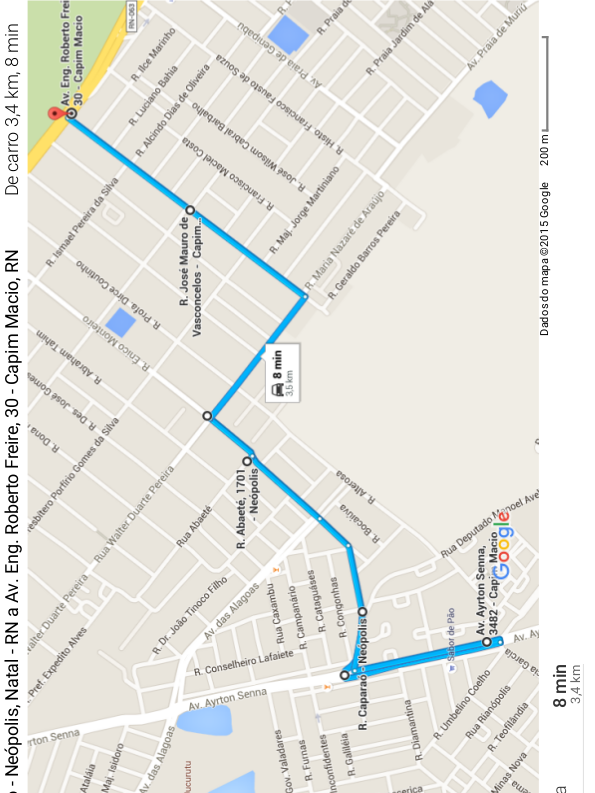
\includegraphics[scale=1.0]{passeio1.png}
	\end{center}
	\ABNTEXchapterfont\small{fonte: Google Maps - 2015}
\end{mapa}
\newpage
\begin{foto}[!htpb]
	\caption{\label{FotoA}O “paradigma de Zimbardo” na av. Ayrton Senna - Neópolis - 13.9.2015}
	\begin{center}
		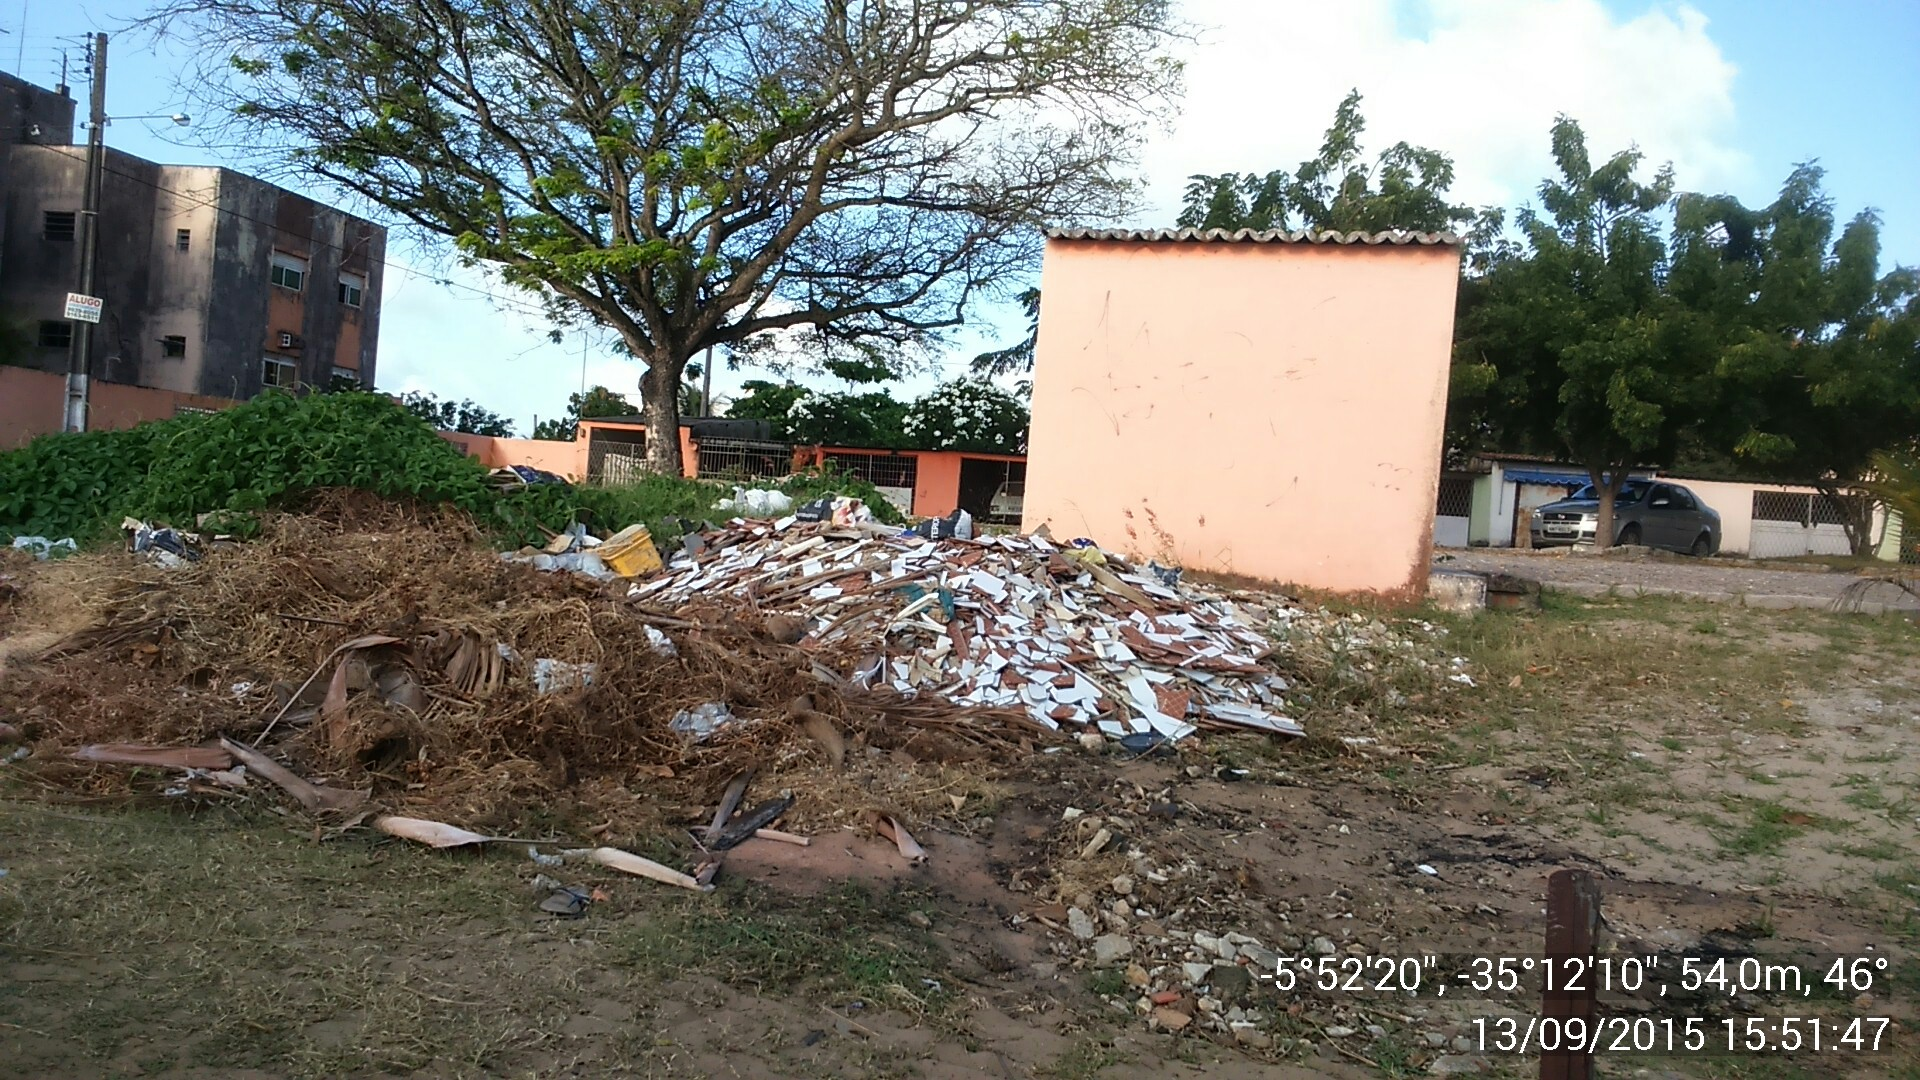
\includegraphics[scale=0.23]{ayrton_senna.png}
	\end{center}
	\ABNTEXchapterfont\small{fonte: próprio autor}
\end{foto}
\begin{foto}[!htpb]
	\caption{\label{FotoB}O “paradigma de Zimbardo” na rua Caparaó - Neópolis - 13.9.2015}
	\begin{center}
		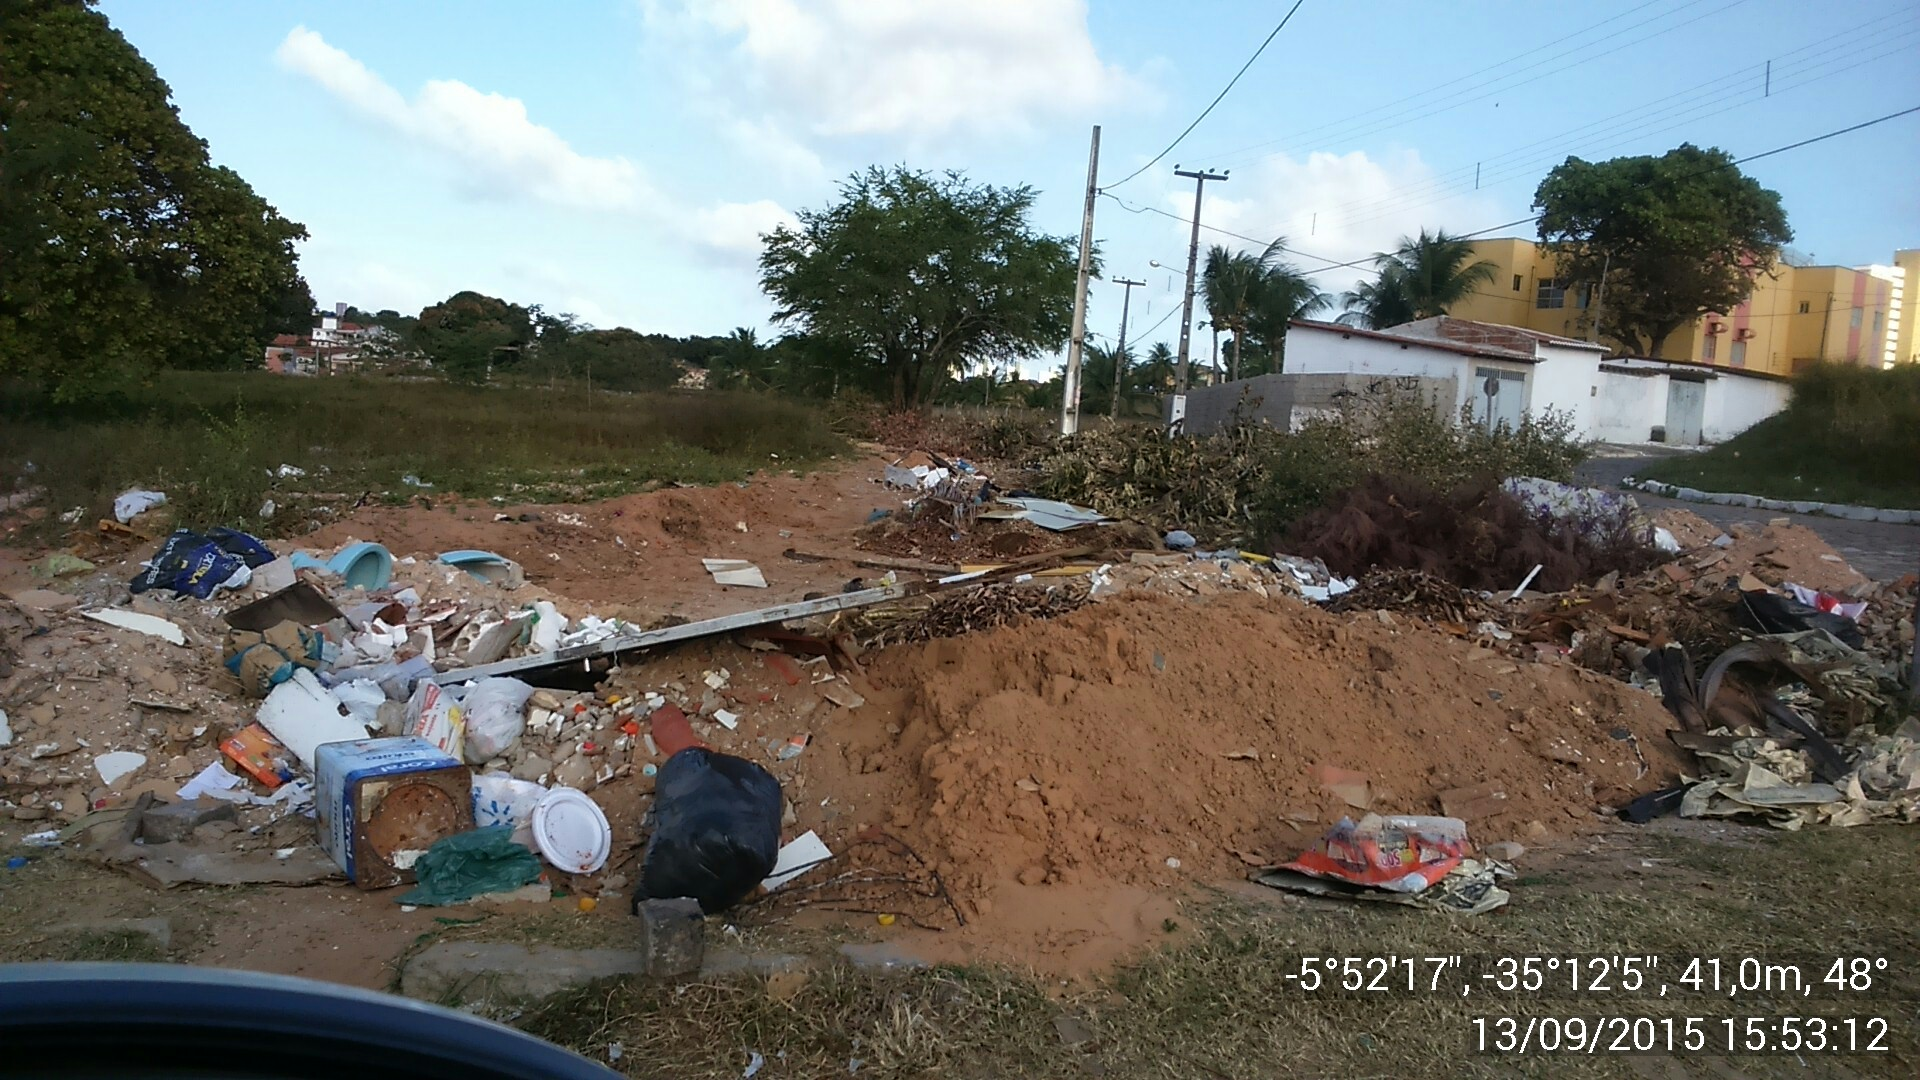
\includegraphics[scale=0.23]{abaete1.jpg}
	\end{center}
	\ABNTEXchapterfont\small{fonte: próprio autor}
\end{foto}
\begin{foto}[!htpb]
	\caption{\label{FotoC}O “paradigma de Zimbardo” na rua Caparaó - Neópolis - 13.9.2015}
	\begin{center}
		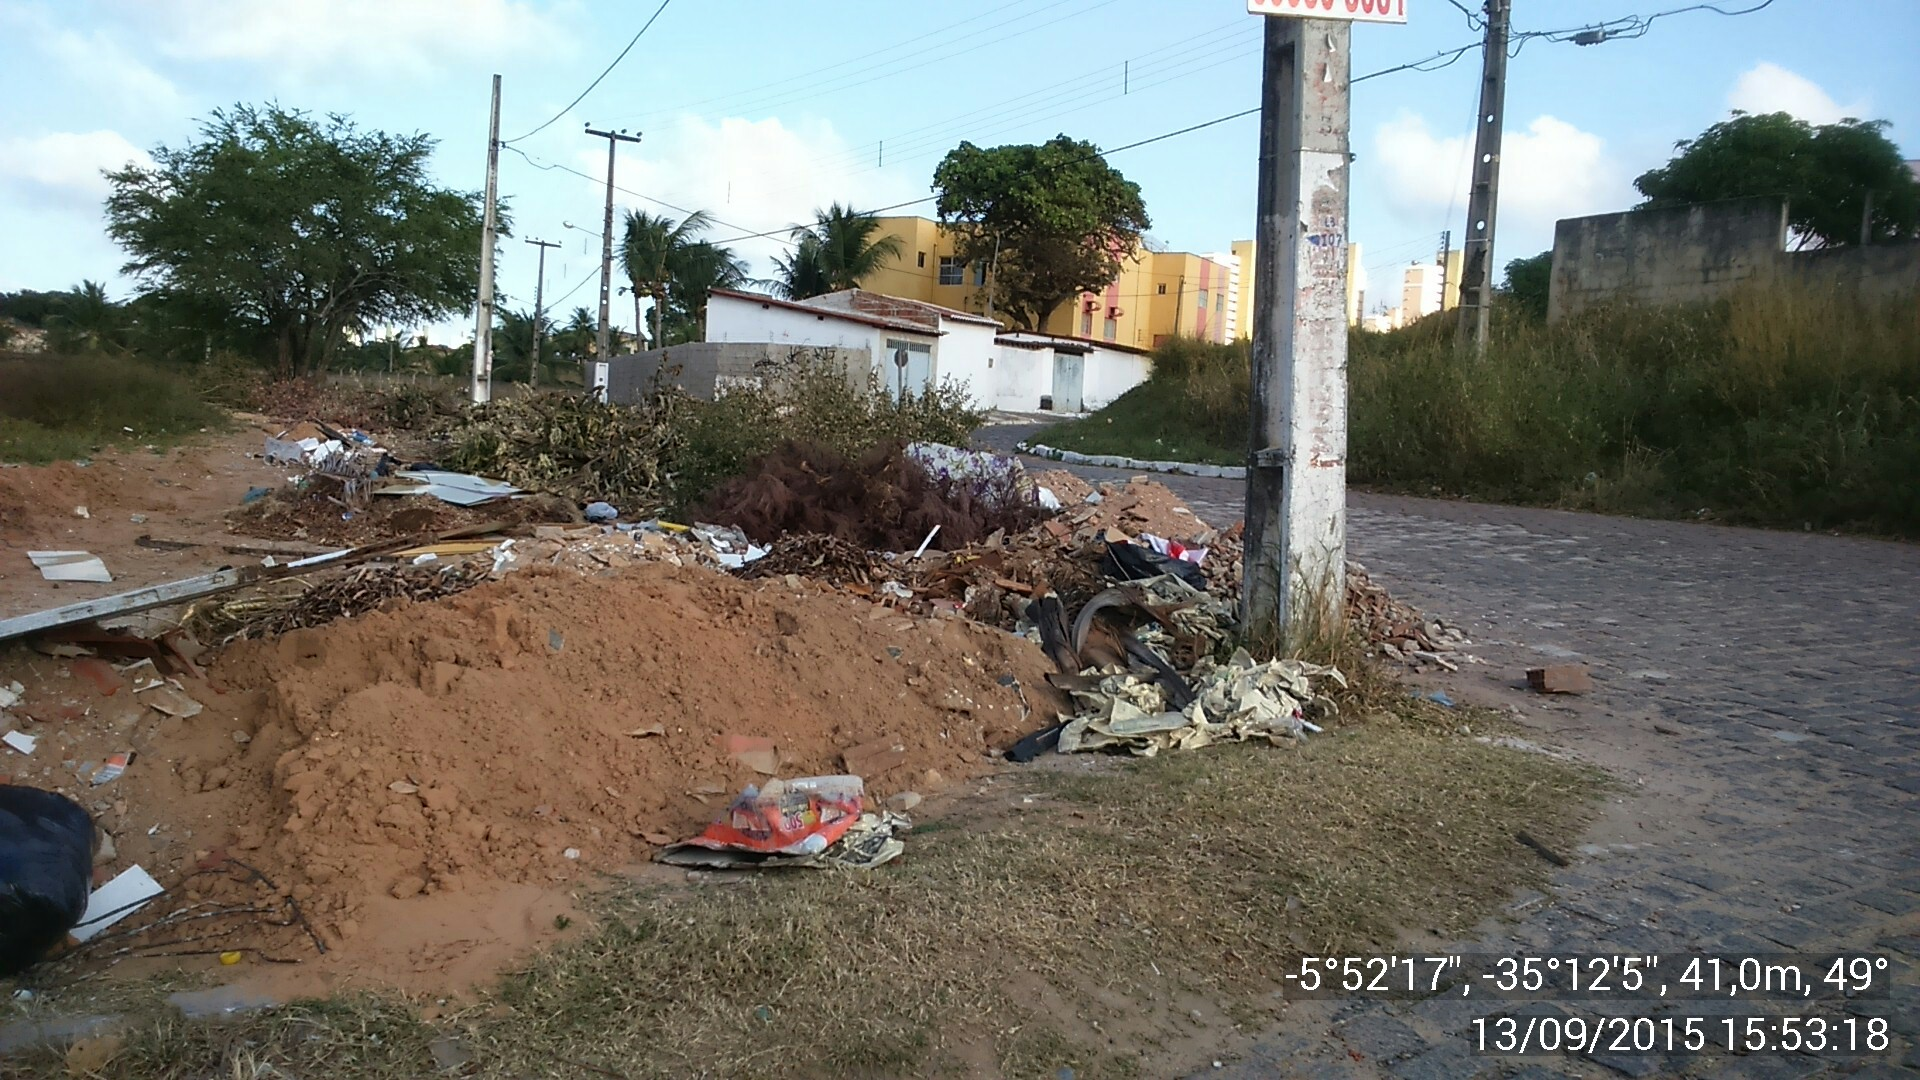
\includegraphics[scale=0.23]{abaete2.jpg}
	\end{center}
	\ABNTEXchapterfont\small{fonte: próprio autor}
\end{foto}
\begin{foto}[!htpb]
	\caption{\label{FotoD}O “paradigma de Zimbardo” na rua Abaeté - Neópolis - 13.9.2015}
	\begin{center}
		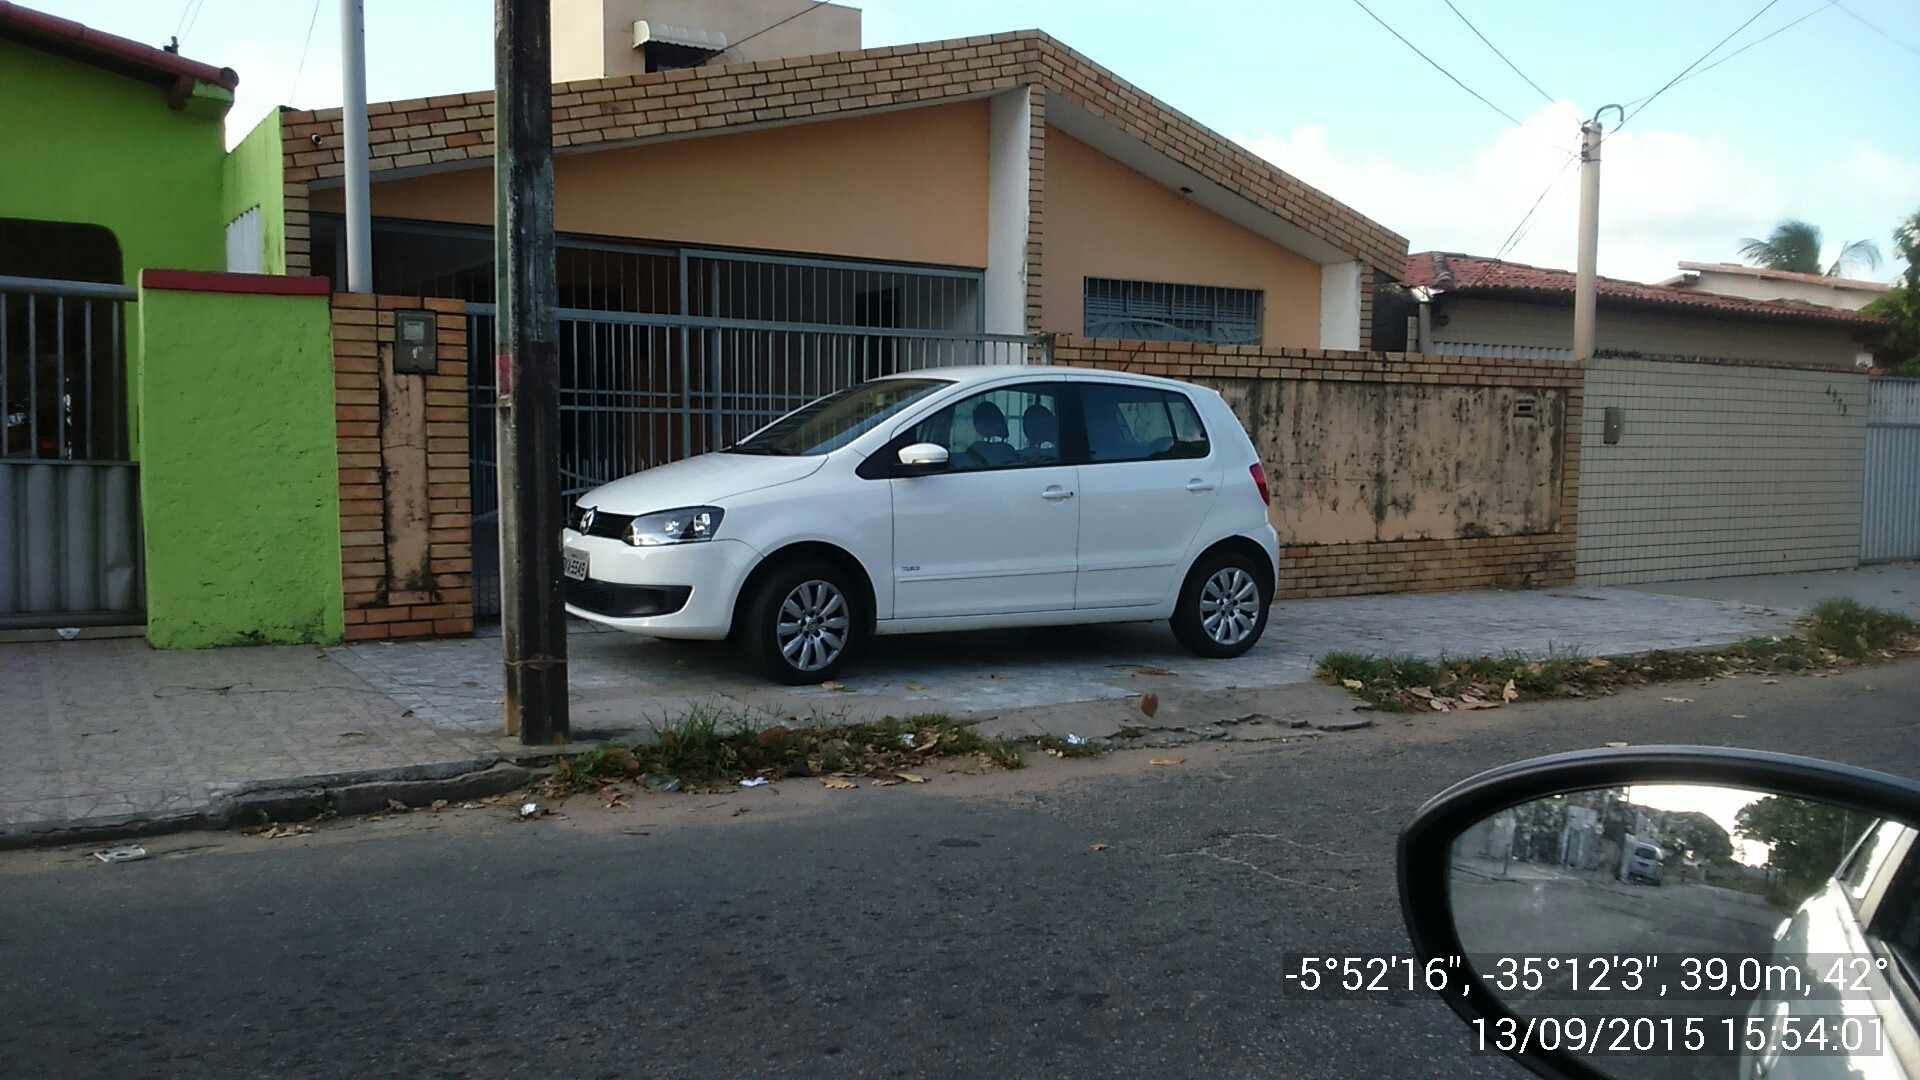
\includegraphics[scale=0.23]{abaete3.jpg}
	\end{center}
	\ABNTEXchapterfont\small{fonte: próprio autor}
\end{foto}
\begin{foto}[!htpb]
	\caption{\label{FotoE}O “paradigma de Zimbardo” na rua Abaeté - Neópolis - 13.9.2015}
	\begin{center}
		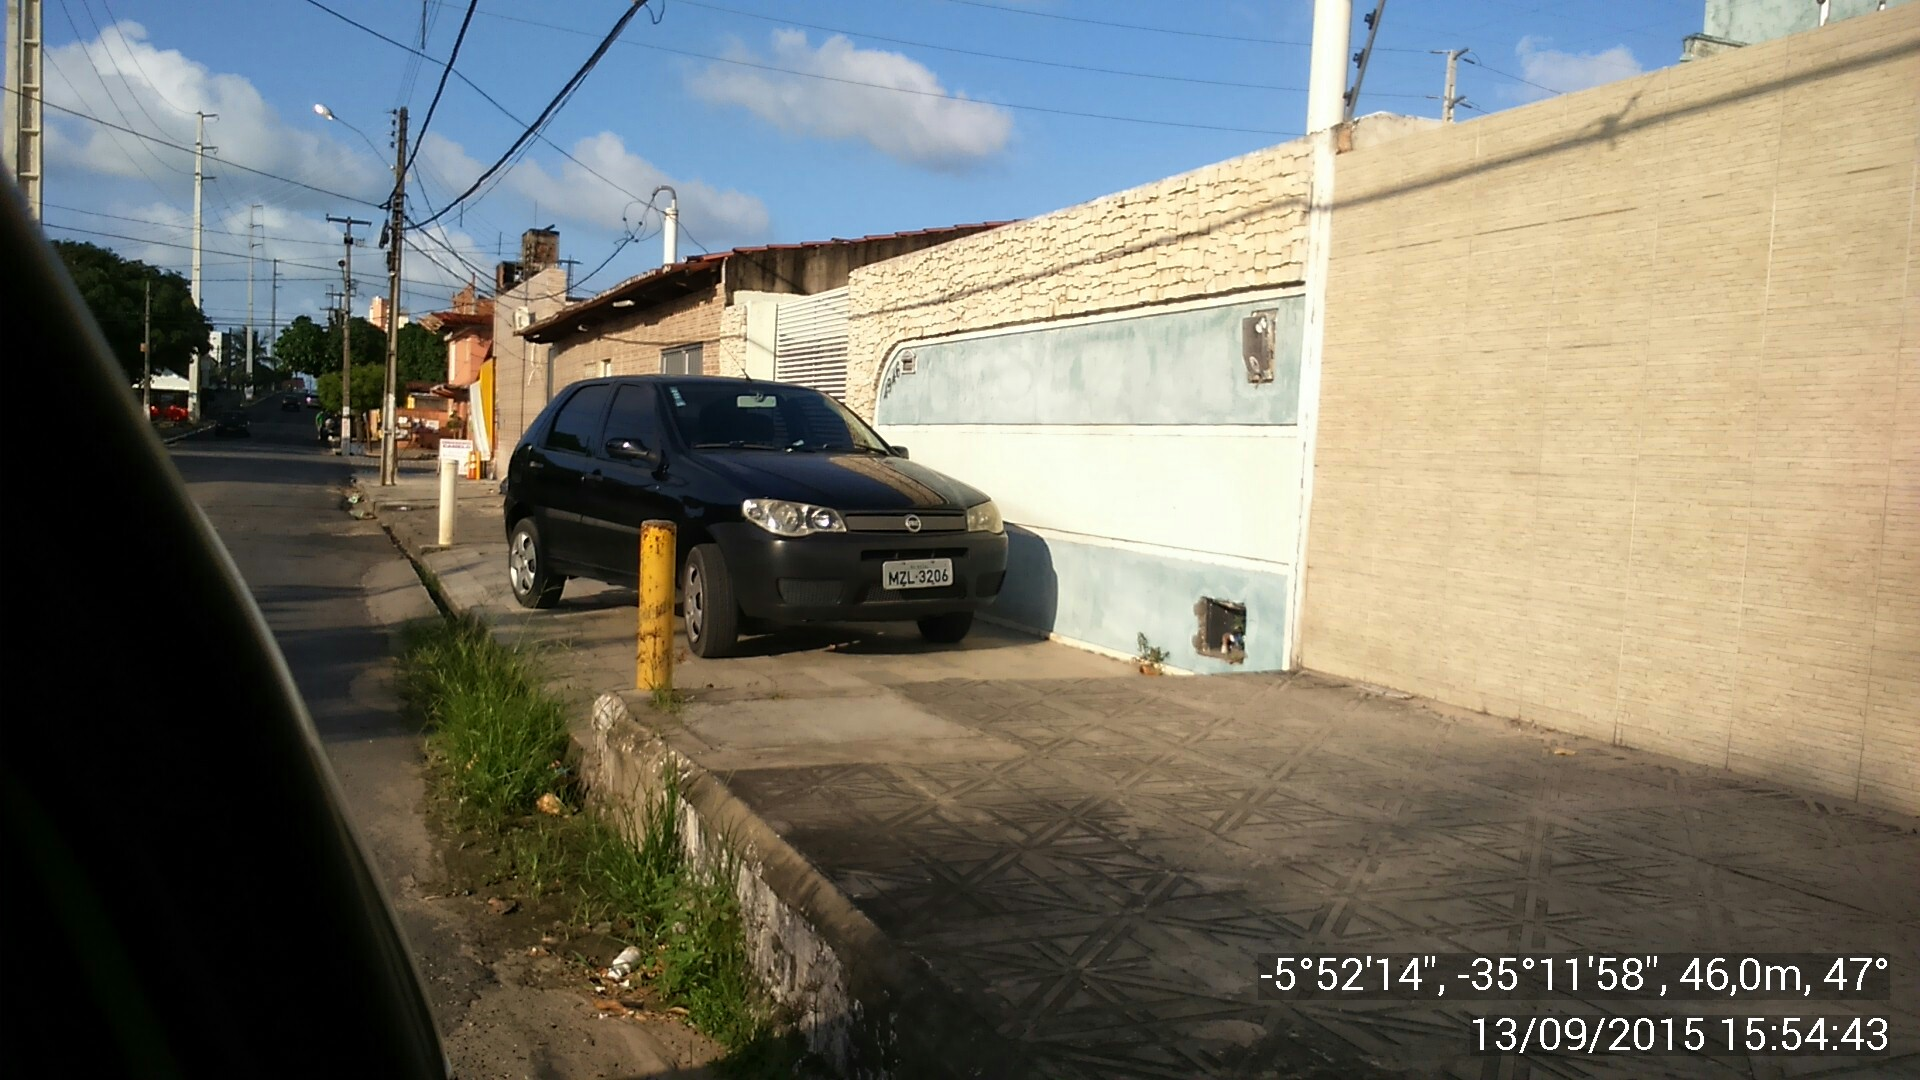
\includegraphics[scale=0.23]{abaete4.jpg}
	\end{center}
	\ABNTEXchapterfont\small{fonte: próprio autor}
\end{foto}
\begin{foto}[!htpb]
	\caption{\label{FotoF}O “paradigma de Zimbardo” na rua Abaeté - Neópolis - 13.9.2015}
	\begin{center}
		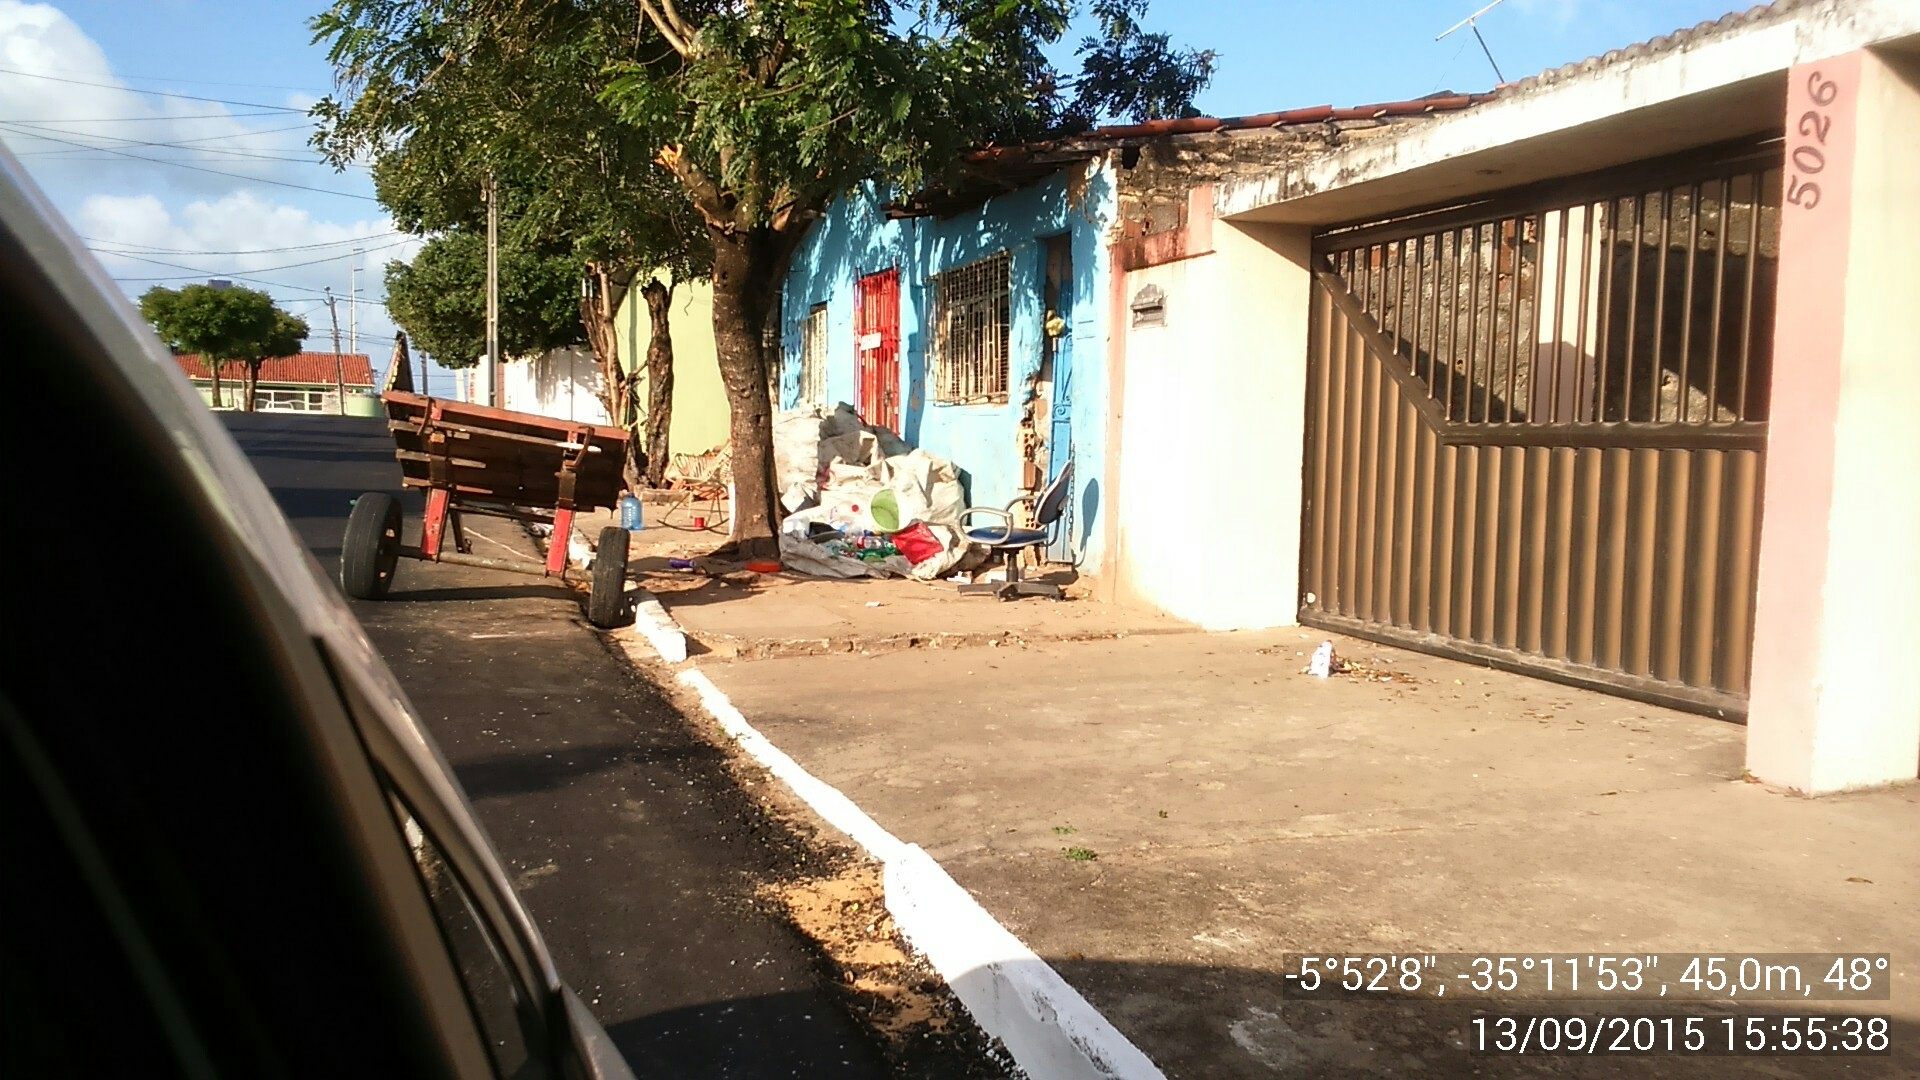
\includegraphics[scale=0.23]{abaete5.jpg}
	\end{center}
	\ABNTEXchapterfont\small{fonte: próprio autor}
\end{foto}

\begin{foto}[!htpb]
	\caption{\label{FotoG}O “paradigma de Zimbardo” na rua Walter Duarte Pereira - Capim Macio - 13.9.2015}
	\begin{center}
		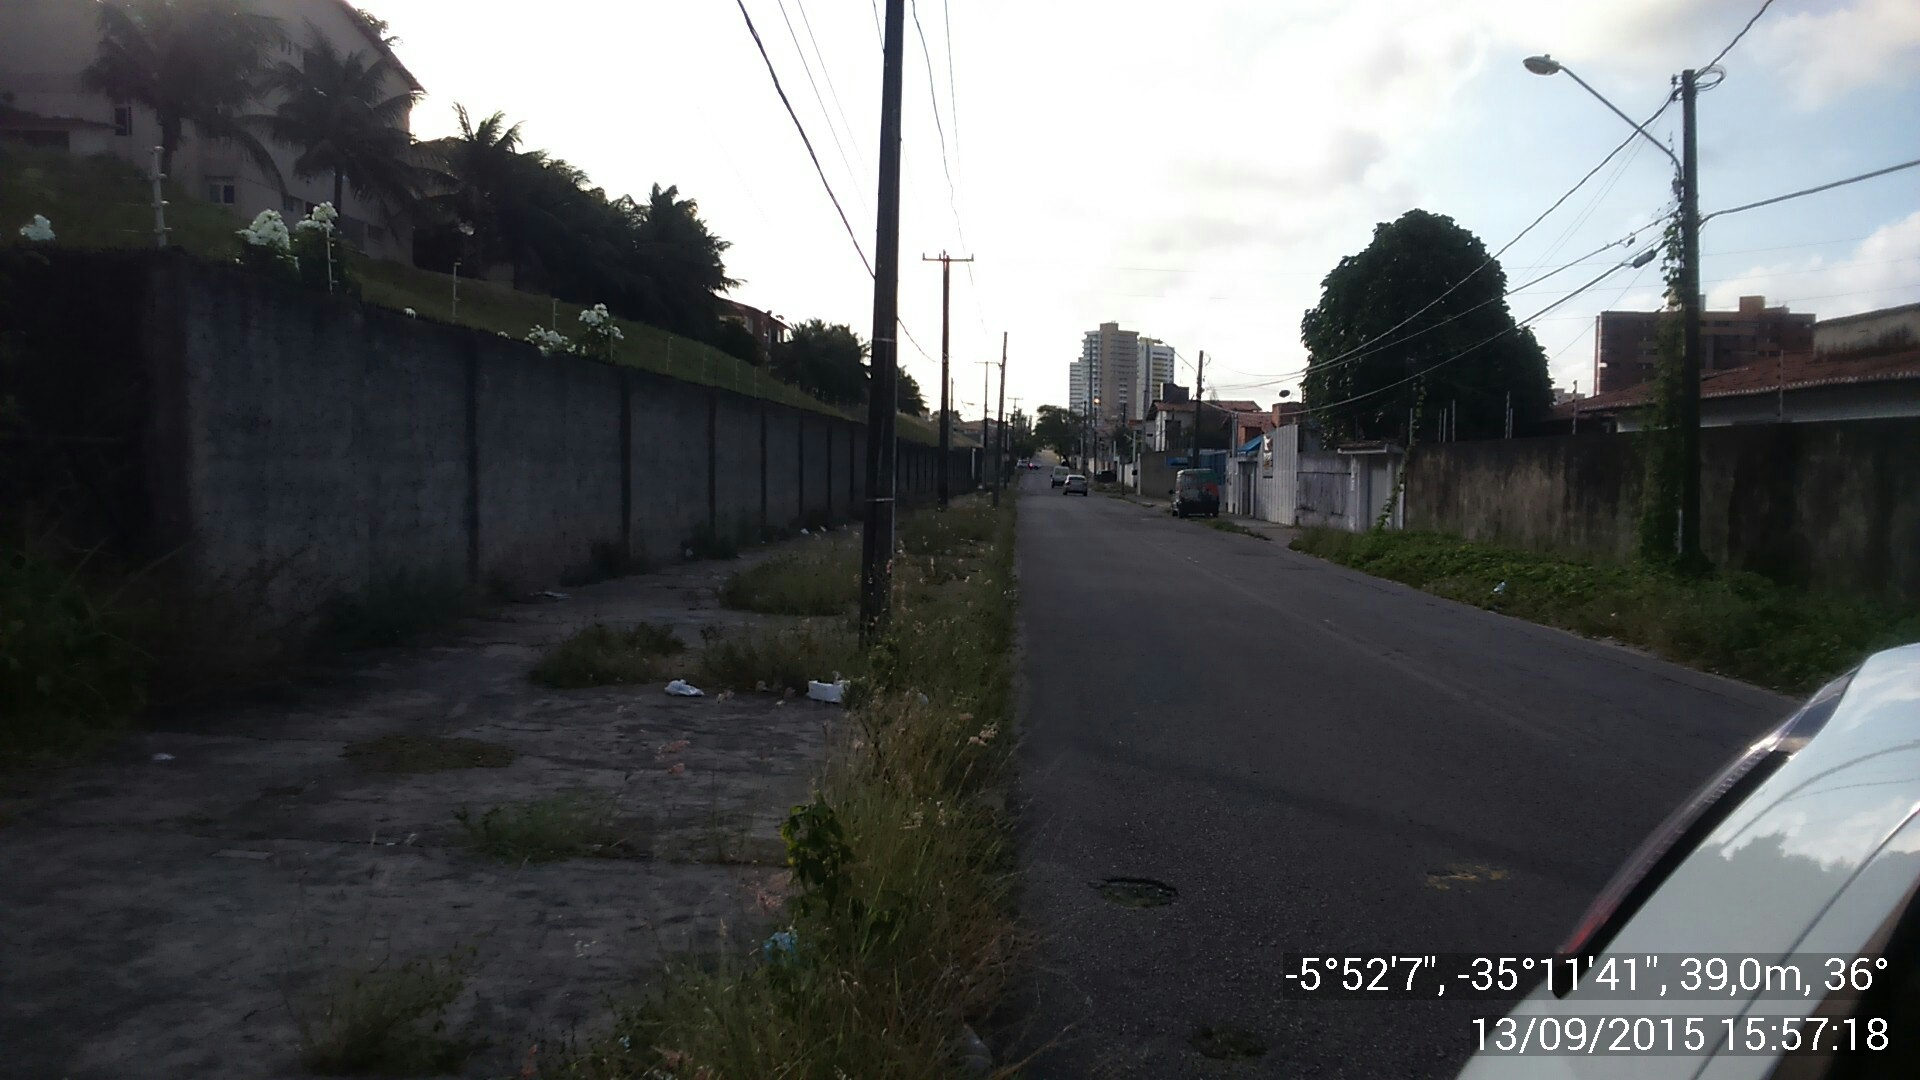
\includegraphics[scale=0.23]{walter1.jpg}
	\end{center}
	\ABNTEXchapterfont\small{fonte: próprio autor}
\end{foto}
\begin{foto}[!htpb]
	\caption{\label{FotoH}O “paradigma de Zimbardo” na rua Walter Duarte Pereira - Capim Macio - 13.9.2015}
	\begin{center}
		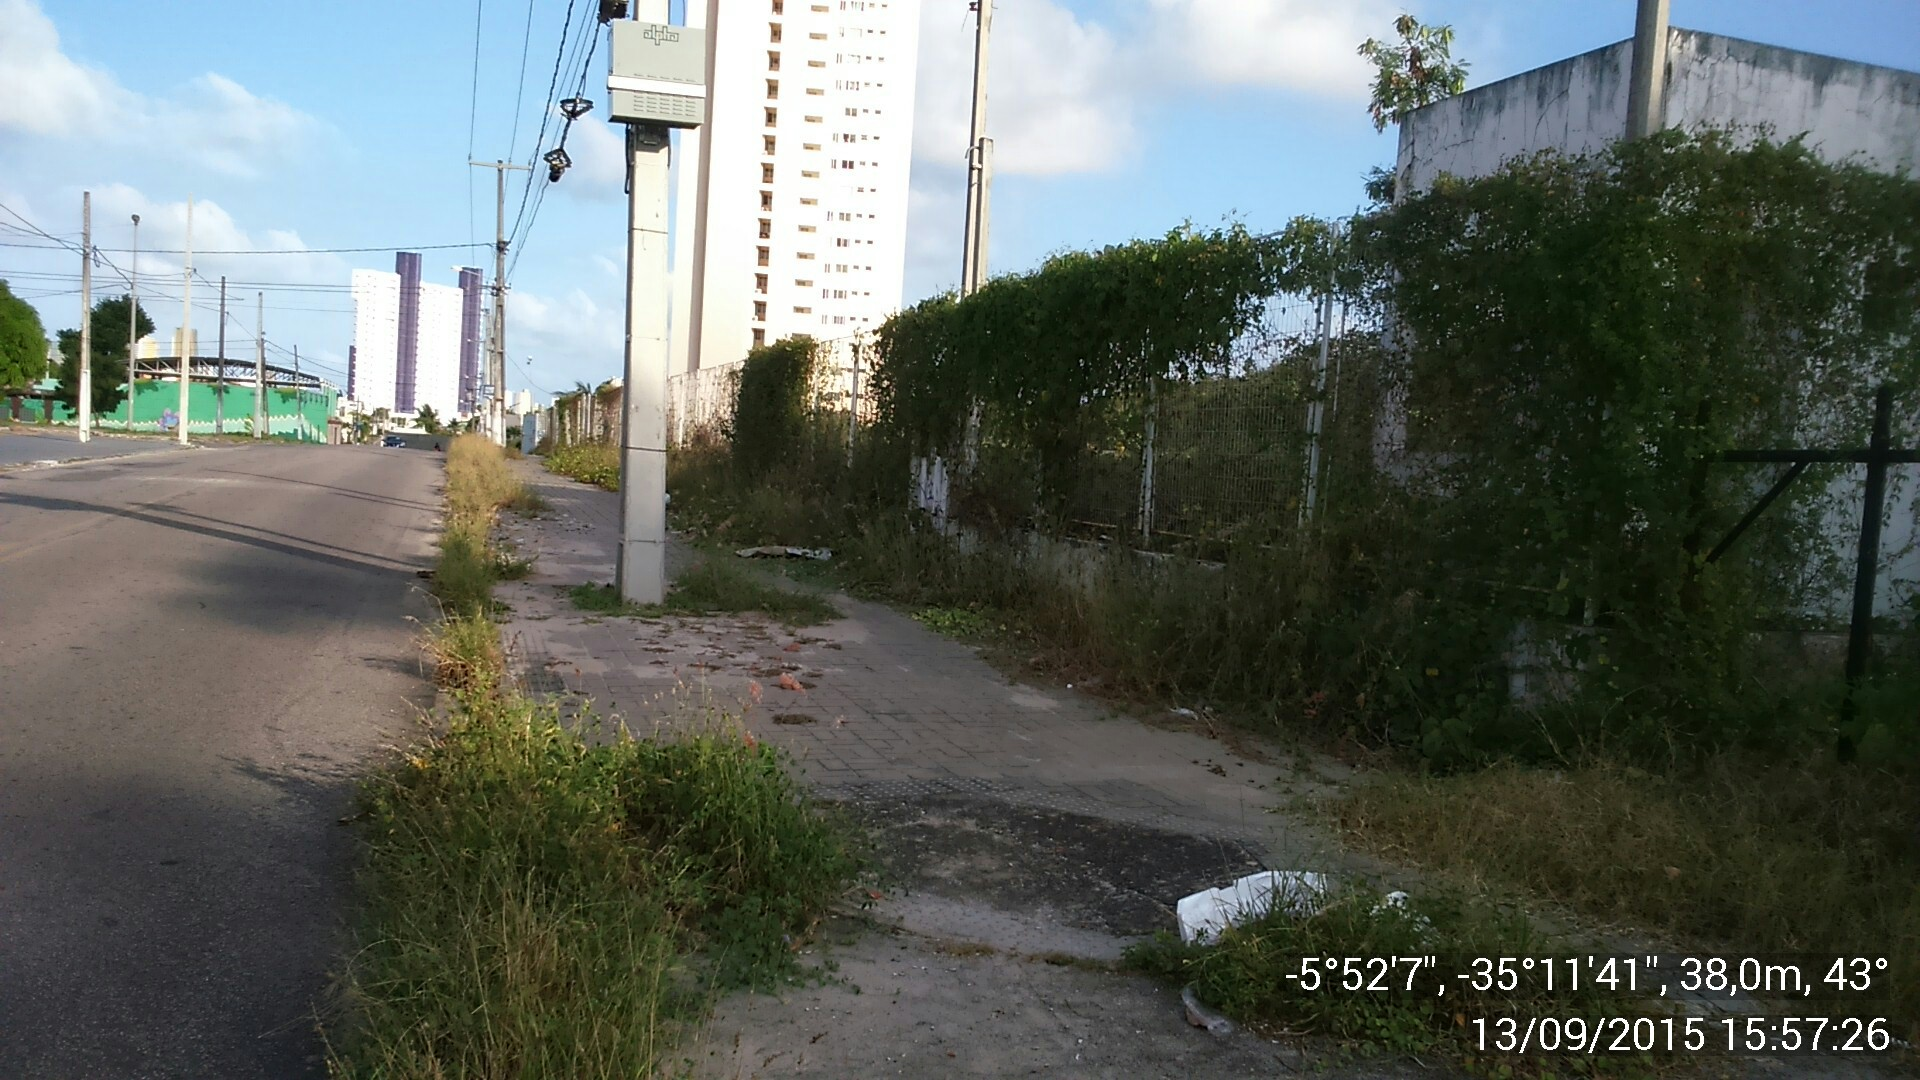
\includegraphics[scale=0.23]{walter2.jpg}
	\end{center}
	\ABNTEXchapterfont\small{fonte: próprio autor}
\end{foto}
\begin{foto}[!htpb]
	\caption{\label{FotoI}O “paradigma de Zimbardo” na rua José Mauro de Vasconcelos - Capim Macio - 13.9.2015}
	\begin{center}
		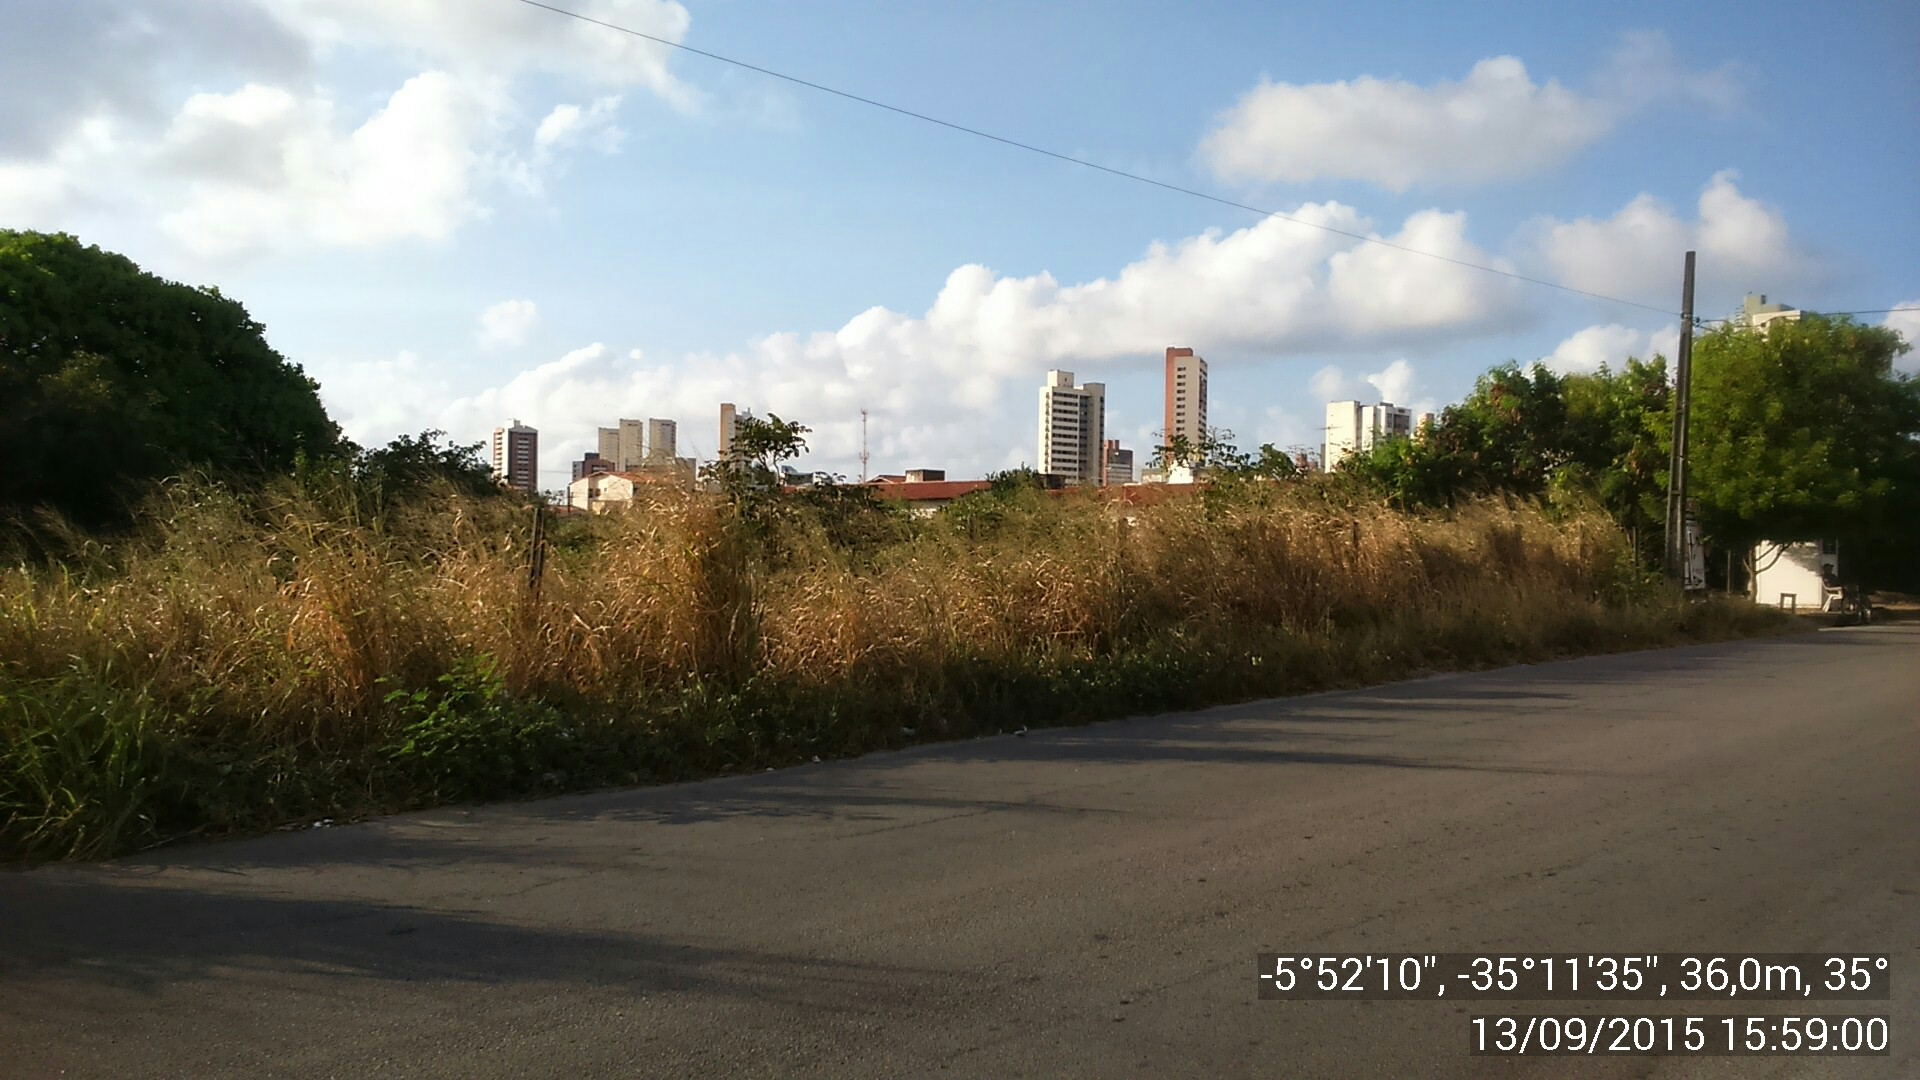
\includegraphics[scale=0.23]{Mauro1.jpg}
	\end{center}
	\ABNTEXchapterfont\small{fonte: próprio autor}
\end{foto}

\begin{foto}[!htpb]
	\caption{\label{FotoJ}O “paradigma de Zimbardo” na rua José Mauro de Vasconcelos - Capim Macio - 13.9.2015}
	\begin{center}
		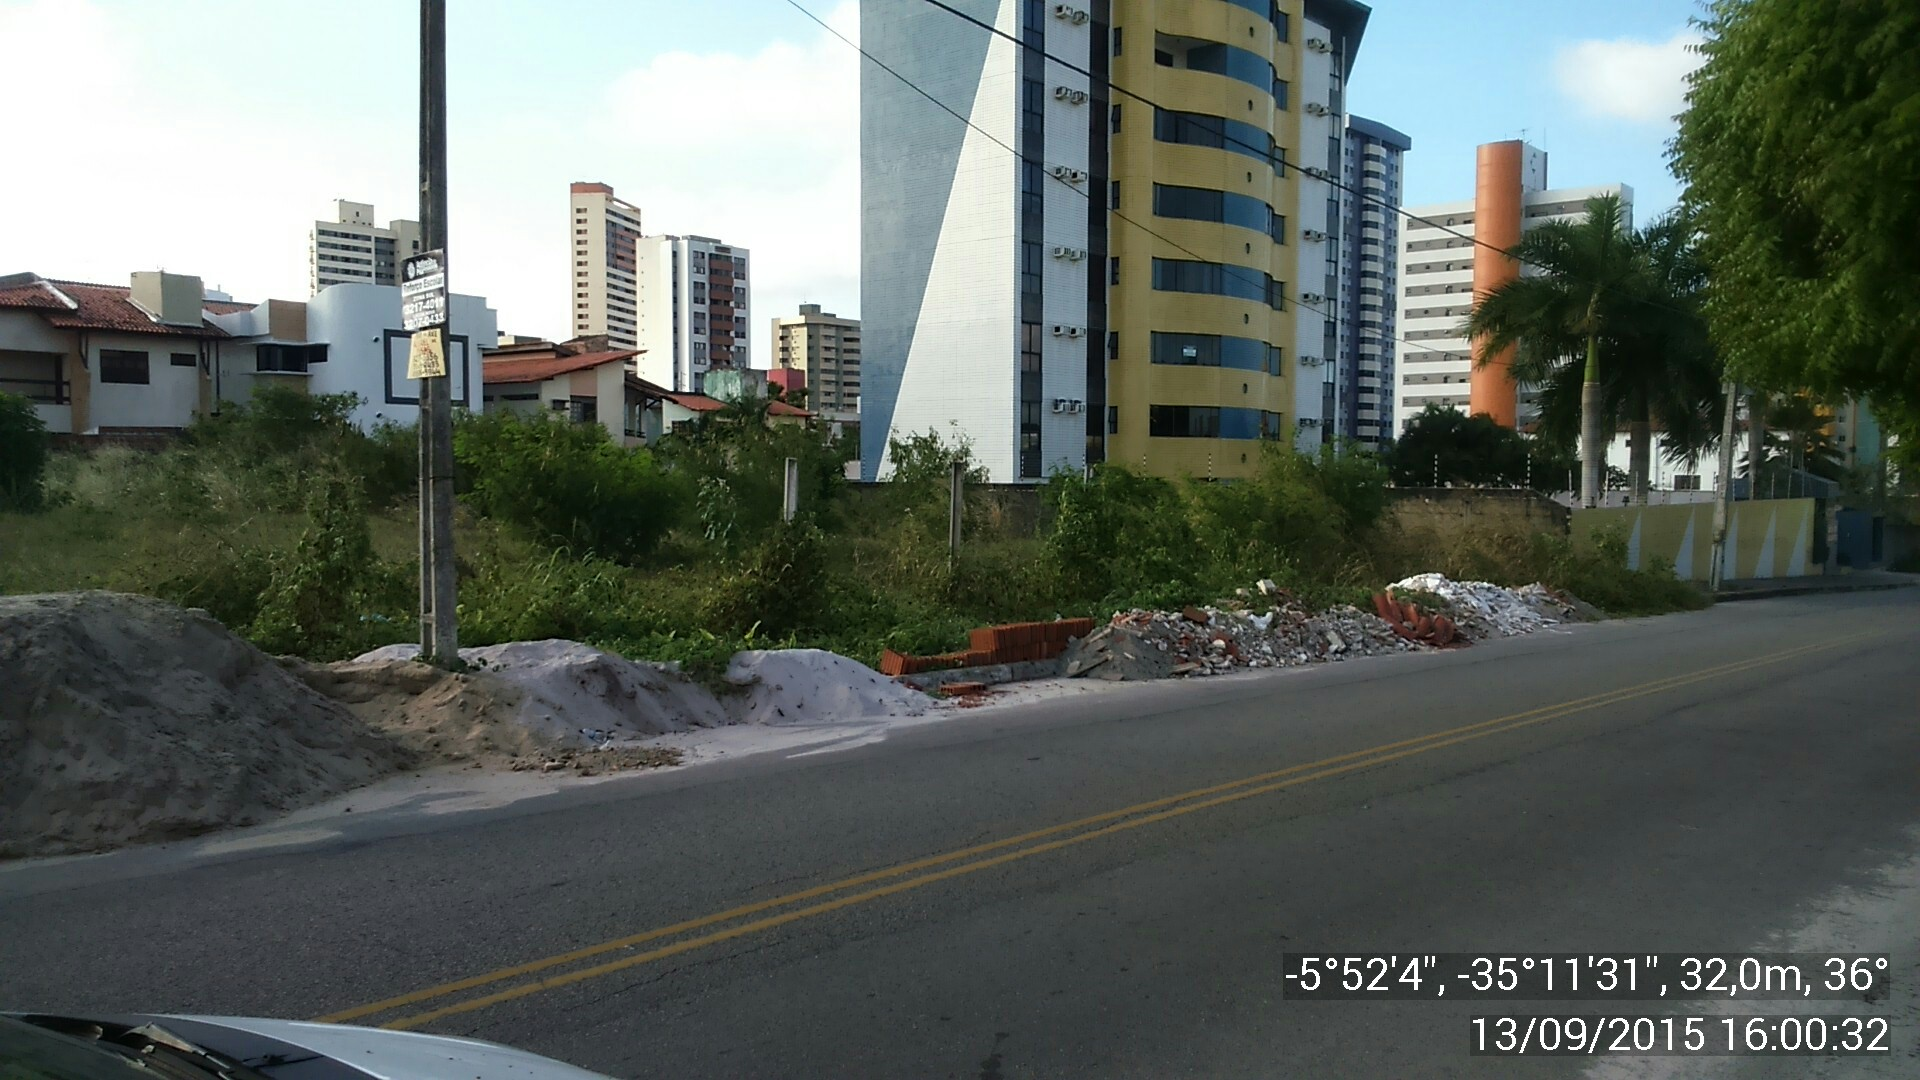
\includegraphics[scale=0.23]{Mauro2.jpg}
	\end{center}
	\ABNTEXchapterfont\small{fonte: próprio autor}
\end{foto}
\begin{foto}[!htpb]
	\caption{\label{FotoK}O “paradigma de Zimbardo” na rua José Mauro de Vasconcelos - Capim Macio - 13.9.2015}
	\begin{center}
		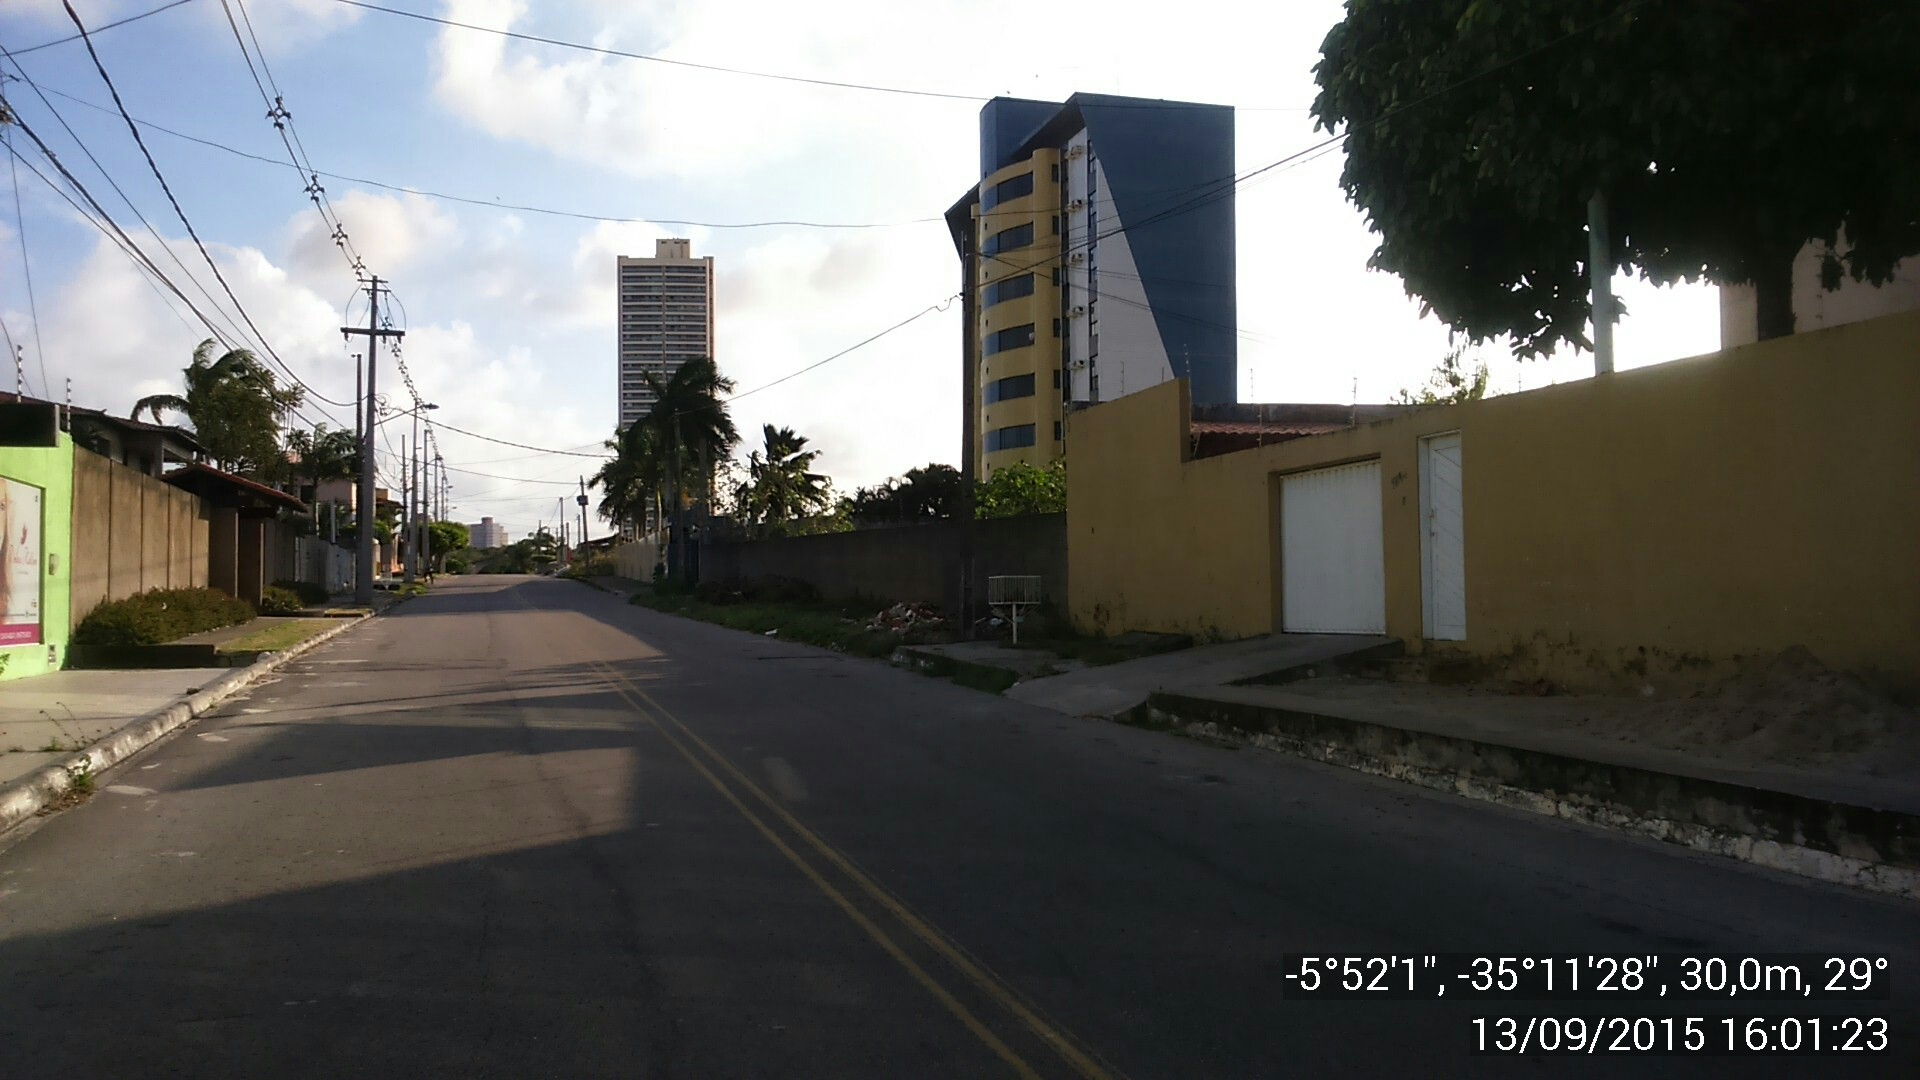
\includegraphics[scale=0.23]{Mauro3.jpg}
	\end{center}
	\ABNTEXchapterfont\small{fonte: próprio autor}
\end{foto}
\begin{foto}[!htpb]
	\caption{\label{FotoL}O “paradigma de Zimbardo” na rua José Mauro de Vasconcelos - Capim Macio - 13.9.2015}
	\begin{center}
		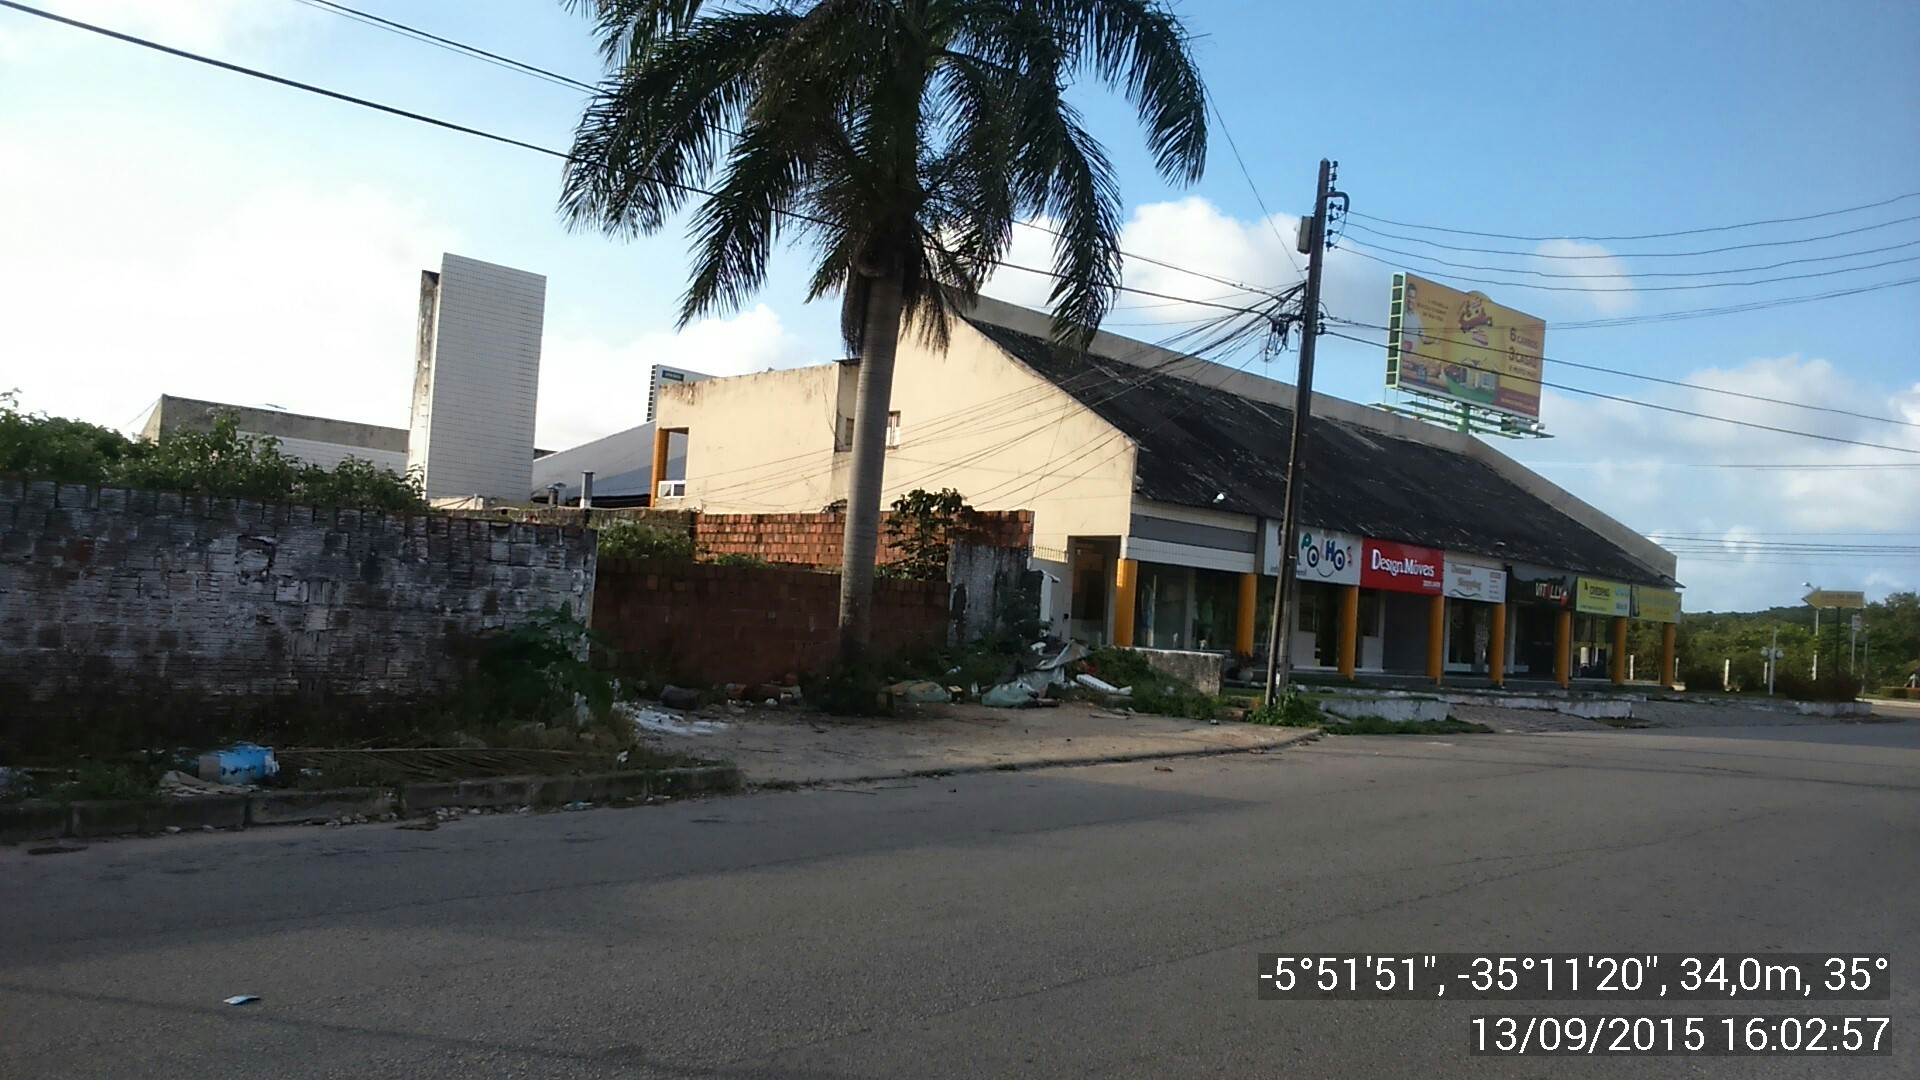
\includegraphics[scale=0.23]{Mauro4.jpg}
	\end{center}
	\ABNTEXchapterfont\small{fonte: próprio autor}
\end{foto}
\end{anexosenv}
\newpage
\thispagestyle{plain}
\paragraph*{\textbf{Como referenciar o presente trabalho:}}

No formato ABNT:\\
GODOY, M. H. \textit{Entre o desvio, o crime e a tolerância zero: estudo da percepção ao
cumprimento das leis no município de Natal-RN}. 165 p. Monografia (Monografia em Gestão
de Políticas Públicas) — Universidade Federal do Rio Grande do Norte, Natal - RN, 2015.


No formato BIBTEX:
\begin{verbatim}
@monography{Godoy,
author	=	{Godoy, Moacir Hardt},
title	=   {Entre o desvio, o crime e a tolerância zero: estudo da percepção 
ao cumprimento das leis no município de Natal-RN},
year	=	{2015},
pages	=	{165},
type	=	{Monografia em Gestão de Políticas Públicas},
school	=	{Universidade Federal do Rio Grande do Norte},
address	=	{Natal - RN},
}
\end{verbatim}
%---------------------------------------------------------------------
\end{document}
